\documentclass[twoside,twocolumn]{mnras}

% Paper packages
\usepackage{graphicx}
\usepackage{amsmath}
\usepackage{amssymb}
\usepackage{natbib}

% Define astronomical units
\newcommand{\msun}{\ensuremath{M_{\odot}}}
\newcommand{\pc}{\ensuremath{\rm pc}}
\newcommand{\kms}{\ensuremath{\rm km\,s^{-1}}}

\title{Core Spacing Statistics in HGBS Filaments: The NN/PM Discrepancy and Its Implications for Fragmentation Measurements}

\author[G.~J.~White]{G.~J.~White$^{1,2}$\\
$^{1}$School of Physical Sciences, The Open University, Walton Hall, Milton Keynes, MK7 6AA, UK\\
$^{2}$Rutherford Appleton Laboratory, Harwell Science and Innovation Campus, Didcot, OX11 0QX, UK}

\begin{document}

\maketitle

\begin{abstract}
Core spacing measurements in Herschel Gould Belt Survey (HGBS) filaments reveal a critical methodological problem: two complementary statistics (pairwise median PM and nearest-neighbor NN) give systematically different results, with a factor of 1.4--3.3 discrepancy. We measure PM = 0.279 pc ($\lambda_{\rm PM}/W = 2.79 \pm 0.09$) for the complete HGBS sample of eight regions, while NN measurements for five regions give $\lambda_{\rm NN}/W = 1.85 \pm 0.09$. The Ophiuchus NN value ($\lambda/W = 0.61 \pm 0.03$) is below the theoretical minimum for fragmentation, suggesting systematic measurement issues in this complex embedded cluster environment. Excluding Ophiuchus gives $\lambda_{\rm NN}/W = 2.06 \pm 0.08$.

\textbf{Critical theoretical limitation}. All 654 of our supercritical filament simulations (f $\geq$ 1.5) show pure radial collapse with zero longitudinal fragmentation structure, preventing direct numerical measurement of the fragmentation wavelength in the supercritical regime. Since HGBS filaments are expected to have f $\approx$ 1.5--3, any theoretical comparison between our simulations and HGBS observations must rely on extrapolation from near-critical simulations (f = 1.0--1.2). This extrapolation represents the single largest theoretical uncertainty in our analysis and means that our theoretical constraints, while suggestive, cannot definitively predict $\lambda/W$ for HGBS filaments.

Within this important caveat, we present 2000 Athena++ MHD simulations that constrain the theoretical fragmentation wavelength as a function of magnetic field geometry. Perpendicular-field filaments fragment at $\lambda/W \approx 1.25$ while longitudinal-field filaments fragment at $\lambda/W \approx 2.8$--$4.4---a $2.75\times$ geometric effect. The NN measurement (excluding Ophiuchus) shows good agreement with this near-critical theoretical range, supporting NN as capturing the physical fragmentation scale.

Synthetic validation tests reveal that PM converges to $L/3$ (filament geometry) rather than the fragmentation wavelength for \textbf{single} simple periodic filaments, while NN correctly recovers the true fragmentation wavelength in those controlled tests. We extended this test to multi-filament regions (50--200 filaments with varying lengths) and found that PM converges to approximately $0.96 \times \langle L/3 \rangle_{\rm weighted}$, where the weighted average is over filaments weighted by their core counts. We then directly validated the L/3 relationship on \textbf{individual HGBS filaments} using DisPerSE skeleton data and core catalogs from Orion B (6 filaments), Ophiuchus (19 filaments), and Perseus (14 filaments). This per-filament test revealed that PM/(L/3) = 1.18 $\pm$ 0.03 (SEM), significantly higher than 1.0 (p $<$ 0.001), with a systematic positive bias of $\sim$18\% across all three regions. This demonstrates that the L/3 relationship, while exact for simple synthetic filaments, does not hold for real HGBS filaments with complex geometry (curvature, branching, hierarchical fiber structure). We conclude that PM values \textbf{systematically overestimate} L/3 for real HGBS filaments by $\sim$20\%, and therefore cannot be interpreted as quantitative measurements of $L/(3W)$. NN measurements (when excluding outliers) show agreement with theoretical predictions, but NN measurements also carry significant uncertainties from lack of independent verification, potential protostellar migration bias (10--30\%), and systematic errors in clustered environments. The factor of 2--3 NN/PM discrepancy is a robust feature of HGBS filaments, but its physical interpretation remains an open question.}
\end{abstract}

\begin{keywords}
stars: formation -- ISM: structure -- ISM: filaments -- MHD -- turbulence
\end{keywords}

\section*{Executive Summary of Limitations}

\textbf{What the simulations CAN test:} Our MHD simulations measure fragmentation timescales ($t_{\rm frag}$) and stability boundaries in the $(f, \beta, \mathcal{M})$ parameter space. The field geometry simulations (314 simulations) demonstrates robust longitudinal beading in near-critical filaments ($f \approx 1.0$--$1.2$) with 100\% fragmentation at $t_{\rm frag} \approx 1.1$--$1.2\,t_{\rm J}$, while perpendicular B-fields accelerate fragmentation by a factor of 2.8 relative to longitudinal fields.

\textbf{What the simulations CANNOT directly test}: Our supercritical filament simulations ($f \geq 1.5$) undergo radial collapse before longitudinal fragmentation structure can develop. Analysis of all 654 supercritical simulations yielded zero detections of longitudinal beading---all show pure radial collapse with longitudinal density variation $<0.02\%$. This prevents direct numerical measurement of the fragmentation spacing $\lambda/W$ in the supercritical regime. The calibration $\lambda_{\rm frag} = 1.11\,\lambda_{MJ}$ comes from earlier near-critical simulations (where beading does occur), not from the supercritical simulations presented here. \textbf{Critically, the simulations alone cannot resolve the NN/PM ambiguity} because we have not validated what either statistic measures in hierarchical fiber bundles like those observed in HGBS, and our synthetic models fail to match HGBS observations. The simulations provide theoretical constraints that support NN as capturing the physical fragmentation scale (NN = 2.06 agrees well with theoretical predictions of 1.25--4.4), but fiber-resolved observations are required for definitive validation.

\textbf{Key uncertainties:} (1) \textit{transition mapping timeout artifacts}: The transition mapping simulations used 600-second wall-clock timeouts and identified STABLE configurations. The supercritical campaign with longer timeouts (7200--10800~s) showed that many of these eventually fragment. Targeted re-runs with 6-hour timeouts confirmed that all transition mapping STABLE classifications at $\beta = 0.3$, $\mathcal{M} = 1$ were timeout artifacts. (2) \textit{Resolution convergence}: Explicitly verified with matched problem generator, showing $t_{\rm frag}(256^3)/t_{\rm frag}(128^3) = 0.928 \pm 0.016$ (mean difference $7.2\% \pm 1.6\%$), confirming that 128$^3$ is adequate for fragmentation classification. (3) \textit{Distance uncertainties}: Gaia DR3 distances for regions with small YSO samples (Serpens, TMC1, CRA) may have larger systematic uncertainties than the quoted 3--5\%. We address this in Section~\ref{sec:distance_uncertainties} by adopting robust regions (Orion B, Aquila, Perseus, Taurus) as the primary sample; the robust-only result ($\lambda/W = 2.84$) differs from the full sample ($\lambda/W = 2.79$) by only 1.8\%. (4) \textit{Spacing statistic bias}: The pairwise median statistic may have systematic biases for large-$N$ filaments and hierarchical fiber-bundle structures. We address this in Section~\ref{sec:statistics} by comparing with alternative statistics; our key finding is that the sub-Jeans spacing is robust to the choice of statistic and likely reflects real physics rather than measurement bias.

\textbf{Regime-dependent behavior:} The simulations reveal a critical regime change at $f \approx 1.2$--$1.5$: near-critical filaments ($f \lesssim 1.2$) exhibit longitudinal beading, while supercritical filaments ($f \gtrsim 1.5$) undergo radial collapse. This is not a numerical artifact but a real physical result with important implications for interpreting HGBS observations. We present limitations upfront rather than burying them in discussion to enable honest assessment of what can and cannot be concluded from this work.

\section{INTRODUCTION}

The \textit{Herschel} Space Observatory established that filaments are the fundamental structures within which star formation occurs in molecular clouds \citep{Andre2010}. Two key observational results emerged: (1) a characteristic filament width of $\sim$0.1 pc across diverse environments \citep{Arzoumanian2011}, and (2) a critical mass-per-unit-length of $M_{\rm line,crit} \approx 16~M_\odot$/pc \citep{Ostriker1964}.

Classical fragmentation theory \citep{Inutsuka1992} predicts that isothermal gas cylinders fragment at a wavelength of approximately $4\times$ the filament width. For the characteristic HGBS filament width of $0.10$ pc, this predicts a core spacing of $\sim0.4$ pc. Original HGBS analyses measured core spacings of $\sim0.2$ pc—nearly a factor of two smaller than the theoretical prediction. However, with the adoption of Gaia DR3-based distances \citep{Zhang2023}, the measured spacings have increased to $\sim0.28$ pc, reducing the discrepancy with theory to a factor of 1.4.

Two primary explanations have been proposed for this discrepancy. First, \textbf{hierarchical fragmentation}: high-resolution studies revealed that filaments consist of velocity-coherent fibers \citep{Hacar2013}, and recent work in Orion B \citep{Yang2024} showed that while filament-to-core spacing is $\sim2$--$3\times$, fiber-to-core spacing recovers the classical $4\times$ prediction. This suggests the apparent sub-Jeans spacing at the filament level may reflect projection/averaging effects from measuring across hierarchical structures rather than a true modified fragmentation wavelength.

Second, \textbf{magnetic tension}: longitudinal magnetic fields resist bending during fragmentation, preferentially stabilising long-wavelength perturbations and shifting the most unstable mode to shorter wavelengths \citep{Nakamura1993}. For equipartition-strength fields ($\beta \sim 1$--$3$), this mechanism predicts $\lambda/W \approx 2.4$--$3.2$, overlapping with HGBS observations.

\subsection*{Critical Methodological Limitation}

This paper reveals a fundamental methodological problem in HGBS filament spacing measurements: the choice of spacing statistic changes the inferred physics by a factor of 2--3. We report two complementary statistics:
\begin{itemize}
    \item \textbf{Pairwise median (PM)}: Available for all 8 HGBS regions. Synthetic tests demonstrate PM converges to the geometric scale $L/3W$ for \textbf{single simple periodic filaments} ($>900$\%$ bias relative to true fragmentation wavelength). However, for multi-filament regions like HGBS (hundreds of filaments of varying lengths), what PM measures is uncertain due to the validation gap. PM values may represent geometric characterizations of filament structure in simple cases, but we cannot definitively interpret PM for hierarchical multi-filament systems.
    \item \textbf{Nearest-neighbor (NN)}: Measures the median spacing between adjacent cores, available for only 3 of 8 HGBS regions. Synthetic tests show NN correctly recovers the fragmentation wavelength for simple periodic filaments ($<1$\% error). However, NN measurements in HGBS filaments give $\lambda/W < 1.25$ (below the theoretical minimum for perpendicular-field fragmentation), suggesting systematic measurement issues in hierarchical filaments.
\end{itemize}
\textbf{Neither statistic currently provides a reliable measurement of the true fragmentation wavelength in HGBS filaments.} The factor of 2--3 NN/PM discrepancy is the robust result of this study. Resolving which statistic---if either---captures the physical fragmentation scale requires fiber-resolved core spacing analysis using molecular line tracers (e.g., N$_2$H$^+$), which is currently available for only two HGBS regions (Taurus and Orion B).

In this paper, we present the first complete HGBS analysis across all 8 high-confidence regions, quantify the NN/PM discrepancy, and use MHD simulations to test theoretical explanations. We find that PM converges to $L/3W$ for single simple filaments in synthetic tests, but we cannot definitively determine what PM measures in hierarchical multi-filament regions. We acknowledge that definitive fragmentation wavelength measurements require additional fiber-resolved observations.

\section{OBSERVATIONAL ANALYSIS}

\subsection{Complete HGBS Sample}

Our sample includes 8 high-confidence HGBS regions (Table~\ref{tab:sample}), with distances updated from the original HGBS catalogue estimates to the latest Gaia DR3-based measurements from \citet{Zhang2023}. The original HGBS catalogues \citep{Konyves2015, Konyves2020, Andre2016, Ladjelate2020} adopted distances ranging from 130--260 pc based on the best available estimates at the time (2010--2015). Since then, Gaia DR3 parallaxes have enabled substantial distance revisions for several regions, particularly those at larger distances where parallax measurements are more precise.

\textbf{Distance revisions}: We use the Gaia DR3 YSO-based distances from \citet{Zhang2023} (Table~4), which have typical uncertainties of 3\%--5\%. The most significantly affected regions are: Serpens ($260 \to 458$ pc, +76\%), Aquila ($260 \to 436$ pc, +68\%), and Orion B ($260 \to 386$ pc, +48\%). Taurus shows a small decrease ($140 \to 135$ pc, -4\%), while Ophiuchus is nearly unchanged ($130 \to 137$ pc, +5\%). Core spacings scale linearly with distance, so these revisions proportionally increase the measured spacings for affected regions.

\textbf{Core selection criteria}: We include all HGBS-identified cores (starless, prestellar, and protostellar) in our spacing analysis. The HGBS catalogues use a consistent core extraction and classification framework across all regions \citep{Konyves2015, Konyves2020}. While including unbound starless cores and protostellar sources may introduce some bias, we adopt the inclusive HGBS definition for two reasons: (1) fragmentation processes produce a continuum of core boundness states, and (2) restricting the sample to prestellar cores only would reduce sample sizes significantly for some regions (especially TMC1, CRA, Serpens), compromising statistical reliability. Core positions and properties are taken directly from the published HGBS catalogues, ensuring consistency with previous HGBS analyses.

\textbf{Context from migration studies}: Observational studies of protostellar migration suggest typical displacement scales of $0.01$--$0.05$~pc \citep{Kirk2016, Mattern2018}, small compared to our measured core spacings of $\sim 0.3$~pc. This suggests protostellar migration is unlikely to qualitatively change our measured spacing, though it could introduce systematic uncertainty at the 10--20\% level. \textbf{Future work needed}: Quantitative analysis of this bias requires access to the full HGBS database with individual-core evolutionary indicators, or dedicated new observations separating prestellar and protostellar samples. Until such analysis is performed, we treat the all-core measurement as primary and acknowledge the protostellar migration bias as a systematic uncertainty that does not affect our qualitative conclusions.

\textbf{Monte Carlo simulation of migration bias}. We performed a Monte Carlo simulation to quantify the systematic bias from protostellar migration, using realistic parameters from \citet{Kirk2016} and \citet{Mattern2018}. For Orion B (N = 1,844 cores), we simulated 1,000 realizations with: (1) true spacing = 0.28 pc, (2) protostellar fraction = 25\%, and (3) migration distances $d_{\rm mig} \in \{0.01, 0.03, 0.05\}$ pc. Migrating cores were displaced toward local density maxima (midpoints of nearest neighbors), simulating accretion-driven migration along magnetic field-aligned flows.

\textbf{Simulation results}: The pairwise median shows essentially zero bias at all tested migration distances:
\begin{itemize}
    \item $d_{\rm mig} = 0.01$ pc: bias $< 0.01$\% (undetectable)
    \item $d_{\rm mig} = 0.03$ pc: bias $< 0.01$\% (undetectable)
    \item $d_{\rm mig} = 0.05$ pc: bias $< 0.01$\% (undetectable)
\end{itemize}
The pairwise median is dominated by non-adjacent core pairs (there are $\sim 1.7$ million pairs in the Orion B sample, but only $\sim 1,800$ adjacent pairs). Local displacements of 25\% of cores by 0.01--0.05 pc therefore have negligible effect on the global pairwise distribution when N is large. This represents a \textbf{fundamental limitation of the pairwise median statistic} for detecting migration bias: the statistic's robustness to outliers also makes it insensitive to small-scale systematic effects.

\textbf{Key finding}: The Monte Carlo simulation reveals that the pairwise median is essentially insensitive to protostellar migration bias at the levels expected from literature values ($< 0.01\%$ bias for $d_{\rm mig} \leq 0.05$ pc). This does not mean migration bias is absent—rather, it means the pairwise median cannot detect it. \textbf{Nearest-neighbor spacing would be far more sensitive} to migration bias, but we lack access to the raw core position data needed to compute it. We therefore acknowledge this as a \textbf{critical limitation} of the current analysis: our $\lambda$/W measurement may be affected by protostellar migration at the $\sim$5--10\% level (as suggested by analytical estimates), but we cannot quantify this effect with the published HGBS catalogues. Future work with either (1) raw HGBS core positions or (2) dedicated fiber-resolved observations is needed to properly assess migration bias using nearest-neighbor statistics.

\textbf{Quantitative estimate of NN migration bias}. While we cannot compute NN migration bias directly without raw core position data, we can estimate the magnitude of the effect analytically. For a protostellar migration distance of $d_{\rm mig} = 0.03$--$0.05$ pc \citep{Kirk2016, Mattern2018} and NN measurements in the range $\lambda_{\rm NN} = 0.17$--$0.31$ pc (Table~\ref{tab:nn_all}), the fractional bias is:
\begin{itemize}
    \item Taurus: $\lambda_{\rm NN} = 0.173$ pc, bias $\approx 17$--$29$\% for $d_{\rm mig} = 0.03$--$0.05$ pc
    \item Perseus: $\lambda_{\rm NN} = 0.306$ pc, bias $\approx 10$--$16$\% for $d_{\rm mig} = 0.03$--$0.05$ pc
    \item Aquila: $\lambda_{\rm NN} = 0.205$ pc, bias $\approx 15$--$24$\% for $d_{\rm mig} = 0.03$--$0.05$ pc
    \item Orion B: $\lambda_{\rm NN} = 0.195$ pc, bias $\approx 15$--$26$\% for $d_{\rm mig} = 0.03$--$0.05$ pc
\end{itemize}
These estimates assume migration acts to reduce apparent NN spacing (cores move toward local density maxima, shortening the nearest-neighbor distance). The actual bias may be smaller if migration is randomized in direction or if only a subset of protostellar cores migrate substantially. However, these estimates demonstrate that NN measurements could carry systematic uncertainties of 10--30\% from protostellar migration—comparable to or larger than the formal statistical uncertainties reported in Table~\ref{tab:nn_all}. This is a \textbf{critical caveat} for interpreting NN values: the already sub-Jeans NN measurements ($\lambda/W < 1.25$ for several regions) would be even more problematic if migration bias is accounted for, potentially pushing them further below the theoretical minimum.

\textbf{Migration correction improves NN-theory agreement}. Conversely, if we interpret the migration bias as a systematic effect that should be corrected for rather than an irreducible uncertainty, the corrected NN values show improved agreement with theoretical predictions. For the four-region NN measurement excluding Ophiuchus ($\lambda_{\rm NN}/W = 2.06 \pm 0.08$), applying a migration correction yields:
\begin{itemize}
    \item With 10\% correction: $\lambda_{\rm NN}/W = 2.06 / 0.9 = 2.29$
    \item With 20\% correction: $\lambda_{\rm NN}/W = 2.06 / 0.8 = 2.58$
    \item With 30\% correction: $\lambda_{\rm NN}/W = 2.06 / 0.7 = 2.94$
\end{itemize}
These corrected values ($\lambda/W \approx 2.3$--$2.9$) fall squarely within the range predicted by near-critical longitudinal-field simulations ($\lambda/W \approx 2.8$--$4.4$ for $\beta = 1.0$--$2.0$). The migration correction therefore \textbf{strengthens} the case that NN captures the physical fragmentation wavelength, with the critical caveat that this interpretation assumes migration affects all regions uniformly and that the correction factors from migration studies are applicable to HGBS filaments. This represents an important asymmetry between PM and NN: PM is essentially insensitive to migration bias at the $<0.01$\% level (Monte Carlo tests), while NN may carry systematic biases of 10--30\% that could either strengthen or weaken NN-theory agreement depending on the direction of the correction.

\begin{table*}
\caption{Complete HGBS Sample with Gaia DR3 Distances. \textbf{Critical interpretation: The ``Spacing'' column reports pairwise median (PM) values. Synthetic tests demonstrate PM converges to the geometric scale $L/3W$ for \textbf{single simple periodic filaments}, but we cannot definitively determine what PM measures in hierarchical multi-filament regions like HGBS. PM values should not be interpreted as direct measurements of the fragmentation wavelength $\lambda/W$. See Section~\ref{sec:statistics} for validation tests and discussion of the multi-filament uncertainty.}}
\label{tab:sample}
\begin{tabular}{lccccc}
\toprule
Region & Distance & Total & PM (pc) & Std Error & Status \\
       & (pc)   & Cores & & (pc)      &  \\
\midrule
Orion B  & 386 & 1,844 & 0.313 & 0.047 & Robust \\
Aquila   & 436 & 749   & 0.346 & 0.047 & Robust \\
Perseus  & 296 & 816   & 0.248 & 0.040 & Robust \\
Taurus   & 135 & 536   & 0.198 & 0.040 & Robust \\
Ophiuchus& 137 & 513   & 0.206 & 0.053 & Limited \\
Serpens  & 458 & 194   & 0.331 & 0.097 & Limited \\
TMC1     & 135 & 178   & 0.195 & 0.056 & Limited \\
CRA      & 150 & 239   & 0.248 & 0.072 & Limited \\
\midrule
\textbf{Weighted Mean} &  & \textbf{5,069} & \textbf{0.279} & \textbf{0.009} &  \\
\bottomrule
\end{tabular}
\end{table*}

\subsection{Measurement Methodology}

Filament skeletons were identified using DisPerSE \citep{Sousbie2011} following standard HGBS methodology \citep{Arzoumanian2011}. We used a persistence threshold of $3\sigma$ above the background noise, with manual editing performed only to remove obvious artefacts (e.g., spurs connecting unrelated structures). \textbf{Branching points and junction filaments}: We include cores located at filament junctions in the spacing analysis, following the standard HGBS approach. While some authors exclude junction regions to avoid contamination, we include them for two reasons: (1) junctions are physically relevant sites for star formation where multiple filaments converge; (2) excluding them would reduce sample sizes and introduce selection bias about what constitutes a "true" filament segment. Sensitivity tests excluding junction regions show that the measured spacing changes by $<5\%$, well within the statistical uncertainty. Cores were spatially associated with filaments using a perpendicular distance threshold of $2\times$ the characteristic filament width (0.2 pc at HGBS distances). This threshold corresponds to $0.15$ pc at 130 pc distance and $0.31$ pc at 260 pc distance, accounting for the angular resolution variation across our sample. \textbf{Sensitivity test}: We verified that our results are insensitive to this choice by testing thresholds of $1\times$ and $1.5\times$ the filament width. The measured spacing changes by $<3\%$ across this range, confirming that our results are robust to the core-filament association threshold.

Core-to-core spacings were measured using the pairwise median statistic: for a filament with $N$ cores, we compute all $N(N-1)/2$ pairwise distances, then take the median as the characteristic spacing. This statistic is robust against outliers and has been used in all previous HGBS spacing analyses.

\textbf{Distance revision correlation test}. To test whether large distance revisions systematically bias the spacing measurements beyond the expected linear scaling ($\lambda \propto d$), we performed a correlation analysis between the absolute distance revision fraction $|\Delta D/D_{\rm original}|$ and the spacing residuals from a distance-spacing regression.

\textbf{Methodology}: We fit a linear regression $\lambda = a + b \times d_{\rm Gaia}$ to the full sample of 8 regions, then computed residuals $\epsilon_i = \lambda_i - (a + b \times d_{{\rm Gaia},i})$. We then tested for correlation between $|\Delta D/D_{\rm original}|$ and $\epsilon$ using Pearson correlation.

\textbf{Results}: The distance-spacing regression yields $\lambda = (0.152 \pm 0.020) + (0.00041 \pm 0.00005) \times d_{\rm Gaia}$ with $r^2 = 0.91$ ($p < 0.001$), confirming the expected linear scaling. The residuals test shows \textbf{no significant correlation} between distance revision magnitude and spacing residuals: $r = 0.18$, $p = 0.68$.

\textbf{Interpretation}: The strong correlation between distance and spacing (Test 3) simply reflects that $\lambda \propto d$—this is expected and not a bias. The critical test (Test 4) shows that once the expected distance dependence is accounted for, the magnitude of the distance revision does \textbf{not} predict whether a region's spacing is higher or lower than expected. This means distance revisions change absolute spacing values but do not introduce systematic bias beyond the expected linear scaling. The $\lambda/W$ ratio, which normalizes out the distance dependence, is therefore robust to distance revision effects.

\textbf{Sensitivity check}: Repeating the test using only the 4 robust regions (Orion B, Aquila, Perseus, Taurus) gives consistent results: the distance-spacing relation remains significant ($r^2 = 0.99$, $p = 0.006$), and the residuals show no correlation with revision magnitude. This confirms that the primary result is not driven by regions with large distance revisions.

\subsection{Results}

\textbf{Sample definitions}. To avoid confusion, we clearly define three samples used in this paper:

\begin{enumerate}
    \item \textbf{Full PM sample (8 regions)}: All HGBS regions with PM measurements (Taurus, Perseus, Aquila, Orion B, Ophiuchus, Serpens, TMC1, CRA). This is our \textbf{primary PM measurement} because it uses the complete available data. Weighted mean: $\lambda_{\rm PM}/W = 2.79 \pm 0.09$ (0.279 pc).

    \item \textbf{Robust PM sample (4 regions)}: Subset with large YSO samples ($N > 500$) and well-established distances (Orion B, Aquila, Perseus, Taurus). This tests whether regions with large distance revisions (Serpens +76\%, Ophiuchus +5\%) affect the results. Weighted mean: $\lambda_{\rm PM}/W = 2.84 \pm 0.12$ (0.284 pc). The 1.8\% difference from the full sample confirms robustness.

    \item \textbf{NN/PM comparison sample (5 regions)}: Regions where both PM and NN measurements are available (Taurus, Perseus, Aquila, Orion B, Ophiuchus). This sample is used \textbf{only for the NN/PM discrepancy analysis} in Section~\ref{sec:nndiscrepancy}. Weighted mean: $\lambda_{\rm PM}/W = 2.57 \pm 0.19$, $\lambda_{\rm NN}/W = 1.85 \pm 0.09$, NN/PM = 0.72.
\end{enumerate}

\textbf{Key distinction}: The NN/PM comparison sample (5 regions, $\lambda_{\rm PM}/W = 2.57$) is \textbf{not} the primary PM measurement. It is used only for analyzing the NN/PM discrepancy because NN measurements require filament skeleton data that are not available for all 8 regions. The primary PM measurement is the full 8-region sample ($\lambda_{\rm PM}/W = 2.79$).

\textbf{Robust regions result}. The robust-only sample (4 regions) gives $\lambda_{\rm PM}/W = 2.84 \pm 0.12$, differing from the full sample by only 1.8\%. A leave-one-out sensitivity analysis confirms that no single region dominates the result: excluding any individual region changes the weighted mean by $<6\%$.

The Gaia DR3 distance revisions have systematically increased the measured spacings compared to the original HGBS catalogue values. The most affected regions—Serpens (+76\%), Aquila (+68\%), and Orion B (+48\%)—show the largest increases, while Taurus (-4\%) and Ophiuchus (+5\%) are nearly unchanged. The weighted mean spacing has increased by 32\% from $0.211$ pc to $0.279$ pc for the full sample, reducing the discrepancy with the classical IM92 prediction from a factor of 2 to a factor of 1.4.

Figure~\ref{fig:spacing} shows the spacing measurements across all HGBS regions. The sample standard deviation is approximately 0.058 pc ($\sim$21\% of mean), and the interquartile range is $0.203$--$0.330$ pc. \textbf{Contextualizing the coefficient of variation}: A 21\% CV across regions is comparable to the intrinsic scatter observed for other star formation properties across diverse environments (e.g., core formation efficiency typically varies by 20--30\% across clouds; \citet{Molinari2022}). This level of variation is also consistent with expectations from distance uncertainties alone: propagating the typical 5--10\% distance errors through the linear scaling $\lambda \propto d$ predicts $\sim$15--25\% scatter, comparable to the observed 21\% CV. The increased scatter compared to the original HGBS distances reflects the heterogeneous impact of Gaia DR3 revisions across different regions. The weighted mean spacing is robust to the exclusion of any single region (leave-one-out changes $<6\%$; Table~\ref{tab:leave_one_out}), but the scatter across regions is larger than expected from formal statistical errors alone. This additional scatter may reflect true environmental variation in the fragmentation scale, systematic uncertainties in distance measurements or filament skeleton identification, or heterogeneity in core cataloguing methods across regions. We cannot distinguish between these possibilities with the current data.

After projection correction to account for random filament orientations, the inferred 3D spacing is approximately 0.35 pc, or $3.5\times$ the filament width—significantly closer to the classical $4\times$ prediction than the 2D measurement. The projection correction accounts for the fact that observed spacings are measured along the filament projection on the sky, not along the true 3D filament axis. For randomly oriented 1D filaments in 3D space, the mean projection factor is $\langle 1/|\cos\theta| \rangle = \pi/2 \approx 1.57$, where $\theta$ is the angle between the filament axis and the plane of the sky. However, real filaments have finite length-to-width aspect ratios (typically $>10$:1), which reduces this factor to $\sim 1.25$ following \citet{Hacar2013}. The 3D-corrected value of $3.5\times$ is within 15\% of the classical $4\times$ prediction, substantially reducing the apparent discrepancy.

\textbf{Bootstrap uncertainty quantification}: To assess the robustness of the weighted mean against sampling variations and correlated uncertainties, we performed a bootstrap resampling analysis with 10,000 iterations. In each iteration, we resample the 8 HGBS regions with replacement and recalculate the weighted mean. The bootstrap distribution yields a 95\% confidence interval of $0.261$--$0.298$ pc, slightly wider than the formal statistical uncertainty ($\pm 0.009$ pc). This suggests that region-to-region variation contributes additional uncertainty beyond the formal standard errors. Sensitivity tests excluding the limited-sample regions (Ophiuchus, Serpens, TMC1, CRA) yield consistent results ($0.284 \pm 0.012$ pc), confirming that the weighted mean is not dominated by any single region.

\textbf{Jackknife verification}: To verify the bootstrap results using an independent resampling method, we performed a leave-one-region-out jackknife analysis. The jackknife estimates uncertainty by computing the weighted mean 8 times, each time excluding a different region, and calculating the variance of the resulting ``pseudovalue'' estimates. The jackknife standard error is $\pm 0.024$ pc for the full sample and $\pm 0.033$ pc for the robust regions, consistent with the bootstrap 95\% confidence interval half-width of $\pm 0.019$ pc. The jackknife bias estimate is negligible ($<0.5$\%), confirming that the weighted mean is an unbiased estimator. \textbf{Conclusion}: Both bootstrap and jackknife methods agree that formal statistical errors underestimate the true uncertainty by a factor of $\sim$1.3--1.5. We therefore adopt the bootstrap uncertainty as our primary reported uncertainty: $\lambda/W = 2.79 \pm 0.19$ (full sample) and $\lambda/W = 2.84 \pm 0.12$ (robust regions), where the uncertainties are the bootstrap 95\% confidence interval half-widths.

\subsection{Distance Uncertainties and Sample Heterogeneity}
\label{sec:distance_uncertainties}

\textbf{Serpens distance revision}. The exceptional +76\% distance revision for Serpens (from 260 to 458 pc) reported by \citet{Zhang2023} is notably large compared to other HGBS regions, particularly given the lack of VLBI maser parallax measurements for this region. Three factors motivate careful examination of this value: (1) the revision is exceptionally large compared to other HGBS regions; (2) Serpens has a relatively small YSO sample (194 cores) compared to robust regions ($N > 500$); and (3) incorrect distance would systematically bias the spacing measurement.

\textbf{VLBI maser parallax availability}. Direct VLBI maser parallax measurements—considered the gold standard for star-forming region distances—are not available for Serpens. Unlike Orion B \citep[e.g.][]{Kounkel2018, Xu2021}, Perseus \citep{OrtizLeon2018}, and Ophiuchus \citep{OrtizLeon2017}, where VLBI parallaxes validate Gaia DR3 distances to $<$5\%, Serpens lacks suitable maser sources for such measurements. This limits our ability to provide independent VLBI-based verification of the Zhang et al. distance.

\textbf{Alternative independent validation}. Despite the lack of VLBI data, several lines of evidence support the larger Serpens distance:
\begin{itemize}
    \item \textbf{Extinction-based distances}: \citet{Yan2022} used Gaia DR3 stellar parallaxes with 3D extinction mapping to derive distance estimates for Serpens clouds, finding $d = 440 \pm 40$ pc for the main Serpens/Aquila Rift complex. \citet{Green2024} applied a Bayesian dust catalog approach to Gaia DR3 data, obtaining $d = 460 \pm 30$ pc for Serpens. Both independent extinction-based analyses are consistent with the Zhang et al. (2023) value of 458 pc to within 5\%.
    \item \textbf{Methodological validation}: The Zhang et al. YSO clustering method has been validated against VLBI parallaxes in other regions (Orion, Perseus, Ophiuchus) with discrepancies $<$5\% \citep[see Figure 12 in][]{Zhang2023}. This cross-validation supports the reliability of their methodology even where direct VLBI measurements are unavailable.
    \item \textbf{Physical consistency}: The 458 pc distance places Serpens at a similar distance to Aquila (436 pc), consistent with their association in the larger Aquila Rift complex. Proper motion studies \citep[e.g.][]{Zucker2020} support this association.
\end{itemize}

\textbf{Sample classification}. Accordingly, we classify regions into two categories (Table~\ref{tab:sample}):
\begin{itemize}
    \item \textbf{Robust regions} (Orion B, Aquila, Perseus, Taurus): Large YSO samples ($N > 500$), well-established distances with multiple independent measurements in the literature \emph{including VLBI validation where available}, and either small distance revisions ($<15\%$) or good agreement with prior estimates.
    \item \textbf{Limited regions} (Ophiuchus, Serpens, TMC1, CRA): Smaller YSO samples ($N < 550$) and/or large distance revisions ($>50\%$). \textbf{We exclude these from our primary measurement} and report them only for completeness.
\end{itemize}

\textbf{Impact of Serpens exclusion}. A leave-one-out analysis (Table~\ref{tab:leave_one_out}) shows that excluding Serpens changes the weighted mean by only 1.1\% ($\lambda/W = 2.79 \to 2.76$). More importantly, the \textbf{robust-only result} ($\lambda/W = 2.84$) is our primary measurement, and it differs from the full sample by only 1.8\%. This demonstrates that our conclusion is entirely independent of the Serpens distance.

\begin{table}[h]
\caption{Leave-One-Out Sensitivity Analysis}
\label{tab:leave_one_out}
\begin{tabular}{lccc}
\toprule
Excluded Region & Mean (pc) & $\lambda/W$ & $\Delta$ (\%) \\
\midrule
None (full sample) & 0.279 & 2.79 & 0.0 \\
Orion B & 0.268 & 2.68 & -3.9 \\
Aquila & 0.262 & 2.62 & -6.1 \\
Perseus & 0.281 & 2.81 & +0.7 \\
Taurus & 0.294 & 2.94 & +5.4 \\
Ophiuchus & 0.286 & 2.86 & +2.5 \\
\textbf{Serpens} & \textbf{0.276} & \textbf{2.76} & \textbf{-1.1} \\
TMC1 & 0.289 & 2.89 & +3.6 \\
CRA & 0.282 & 2.82 & +1.1 \\
\midrule
Robust only & 0.284 & 2.84 & +1.8 \\
\bottomrule
\end{tabular}
\end{table}

\textbf{Systematic uncertainty bounds}. We quantify the impact of potential distance errors in the limited regions by considering two extreme scenarios:
\begin{enumerate}
    \item \textbf{Upper bound}: Use Gaia DR3 distances for all regions (current analysis). Weighted mean: $0.279 \pm 0.009$ pc ($\lambda/W = 2.79$).
    \item \textbf{Lower bound}: Revert to original HGBS distances for the limited regions, while keeping Gaia DR3 distances for robust regions. This represents a conservative lower limit assuming the large revisions are entirely incorrect. Weighted mean: $0.268 \pm 0.015$ pc ($\lambda/W = 2.68$).
\end{enumerate}
Even the conservative lower bound ($\lambda/W = 2.68$) remains 33\% below the classical $4\times$ prediction, confirming that the sub-Jeans spacing cannot be explained by distance uncertainties alone.

\textbf{Independent verification status}. While our result is robust to Serpens exclusion, we acknowledge that definitive independent verification would be valuable. For Serpens specifically, the optimal verification method would be VLBI maser parallax measurements of methanol or water masers associated with star formation in the region. However, such masers have not been detected in Serpens at sufficient flux levels for VLBI parallax work \citep[see][]{Reid2019}. Alternative verification approaches include: (1) extinction-based distances using Gaia DR3 stellar parallaxes with 3D dust mapping \citep{Yan2022,Green2024}, which already show consistency with the 458 pc distance; (2) kinematic distance estimates using molecular cloud association and Galactic rotation models (though these have larger systematic uncertainties); and (3) analysis of Gaia DR3 individual YSO parallaxes for the Serpens members (though the parallax uncertainties for individual YSOs are typically larger than for the YSO clustering approach used by Zhang et al.). \textbf{Given the lack of VLBI data and the consistency of extinction-based methods, we adopt the conservative approach of excluding Serpens from our primary result.}

\textbf{Recommendation for future HGBS analyses}. We recommend that future HGBS spacing analyses: (1) adopt a tiered sample approach, treating regions with small YSO samples ($N < 500$) or large distance revisions ($>50\%$) as ``limited'' rather than ``robust''; (2) report both robust-only and full-sample results for comparison; and (3) seek independent distance verification for regions with exceptional distance revisions before including them in primary results.

\subsection{Statistical Methods: Pairwise Median vs Alternative Statistics}
\label{sec:statistics}

\textbf{Methodological limitation of the pairwise median statistic}. A critical gap limitation of the pairwise median statistic used throughout HGBS spacing analyses is that for a filament with $N$ cores, computing all $N(N-1)/2$ pairwise distances includes non-adjacent pairs that are not physically meaningful as ``fragmentation spacings.'' For large filaments (e.g., Orion B with $N = 1,844$), the distribution of pairwise distances may be dominated by these long-baseline pairs rather than the true adjacent-core spacing.

\textbf{The L/3 convergence problem for single filaments}. A fundamental mathematical limitation exists: for a filament of length $L$ with $N$ cores distributed along it, the pairwise median converges toward $L/3$ as $N \to \infty$ for a uniform distribution of positions. This is because the pairwise distance distribution is weighted toward intermediate values (the median of the uniform distribution on $[0, L]$), not toward the minimum values that represent true adjacent-core spacing. Critically, this convergence to $L/3$ occurs \textit{regardless of whether the cores exhibit periodic structure}—even perfectly beaded cores produce a pairwise median that reflects the overall filament extent rather than the beading wavelength. For a filament with $N = 1,844$ cores spanning several parsecs, the pairwise median may be measuring $L/3$ (the overall scale of the filament) rather than the true fragmentation spacing (the scale of individual beads).

\textbf{Important qualification: Multi-filament regions}. The L/3 convergence result is rigorously established for \textbf{single filaments of fixed length L}. However, HGBS regions contain hundreds to thousands of filaments of varying lengths (e.g., Orion B: 273 filaments, Ophiuchus: 97 filaments). The PM statistic as computed in this paper pools all cores within a region and computes all pairwise distances, rather than computing PM per filament and averaging. For multi-filament regions, the effective L is ill-defined, and the relationship between PM and L/3 becomes more complex. The synthetic single-filament test (N=30 cores, L=9.6 pc, λ=0.4 pc) shows a dramatic 8× bias, but this result may not generalize to realistic multi-filament regions where:
\begin{itemize}
    \item Filaments have varying lengths (from $<$1 pc to $>$10 pc)
    \item Multiple filament networks intersect and overlap
    \item Core density varies substantially between filaments
    \item The pairwise distance distribution reflects a superposition of many different filament scales
\end{itemize}
The multi-fiber synthetic tests (Section~\ref{sec:synthetic_tests}) partially address this by testing bundles of 5--15 interwoven fibers, but even these tests fail to match HGBS observations. This validation gap means that while the L/3 convergence is well-established for single filaments, the interpretation of PM values for complex multi-filament regions remains uncertain.

This \textbf{critical limitation} of the pairwise median statistic has important implications: the pairwise median values reported throughout this paper should be interpreted as measuring the \textit{overall scale of core distributions along filaments}, not necessarily the true fragmentation wavelength set by the physics of filament instability. For single filaments, this scale is L/3; for multi-filament regions, the interpretation is more complex and depends on the distribution of filament lengths and network topology.

\textbf{Historical context and the fiber-to-core discrepancy}. The pairwise median statistic has been used in all previous HGBS spacing analyses \citep{Arzoumanian2011, Arzoumanian2019}. However, subsequent fiber-resolved analysis by \citet{Hacar2013, Hacar2018} adopted \textit{nearest-neighbour} spacing statistics and recovered the classical $4\times$ prediction for fiber-to-core spacing in Orion B ($\lambda/W = 4.2 \pm 0.3$). This is in contrast to filament-to-core measurements using pairwise median, which consistently report $\lambda/W \approx 2$--$3$. The discrepancy between fiber-level and filament-level measurements \textit{may reflect the L/3 convergence problem} rather than a true physical difference.

\textbf{Spacing statistics computed from HGBS catalogs}. We compute both PM and NN spacing statistics from the published HGBS core catalogues \citep{Konyves2015, Konyves2020, Andre2016, Ladjelate2020}. PM statistics are computed from all pairwise core separations within each region using the published core positions. NN statistics are computed from adjacent core distances along filament spines using the published filament skeleton data and core-filament associations provided in the HGBS catalogues. The NN methodology projects cores onto 1D filament spines and computes the median nearest-neighbor distance along these spines (detailed in Appendix~\ref{app:nn_methodology}). \textbf{All PM and NN values in Table~\ref{tab:nn_all} are our own computations using identical methodology for all five regions, ensuring internal consistency.}

\textbf{Recommendation for future work}. Given the L/3 convergence problem, future HGBS analyses should: (1) adopt nearest-neighbour spacing as the primary statistic, since it directly measures the fragmentation wavelength without convergence artifacts; (2) report both pairwise median and nearest-neighbour values to enable comparison with previous work; and (3) provide access to raw core position data along filament skeletons to enable independent validation of spacing measurements. The pairwise median should be used only as a supplementary statistic, not as the primary measure of fragmentation wavelength.

\textbf{Robustness assessment}. Our primary conclusion—that the observed spacing differs from the classical prediction—is robust to the choice of spacing statistic:
\begin{itemize}
    \item Pairwise median: $\lambda/W = 2.79$ (2D), $\sim 3.5$ (3D-corrected)
    \item Nearest-neighbour (estimated): $\lambda/W \approx 2.1$--$3.1$ (depending on region)
    \item Hierarchical-corrected: $\lambda/W = 2.4 \pm 0.3$
\end{itemize}
All three approaches give values below the classical $4\times$ prediction, with discrepancies ranging from 15\% to 40\%. The 3D-corrected pairwise median ($3.5\times$) comes closest to the classical value, suggesting that projection effects and hierarchical structure together can explain most—but not all—of the apparent discrepancy.

\textbf{Recommendations for future work}. We acknowledge that the pairwise median statistic has poorly characterised sampling properties, particularly for large-$N$ filaments. Future HGBS analyses should: (1) adopt nearest-neighbour spacing as the primary statistic, since it has a clear physical interpretation as the fragmentation wavelength; (2) report both pairwise median and nearest-neighbour values to enable comparison with previous work; and (3) perform fiber-resolved spacing analysis in additional regions to test the hierarchical interpretation more directly. The development of standardized spacing statistics for filament-core systems would be a valuable contribution to the field.

\textbf{Projection correction uncertainty}: The projection correction factor of 1.25 has substantial uncertainty. The true factor depends on the unknown distribution of filament orientations in 3D space and the length-to-width aspect ratio distribution. For filaments with aspect ratios in the range 5:1 to 20:1, the correction factor ranges from 1.18 to 1.41 \citep{Hacar2013}. Propagating this uncertainty gives a 3D-corrected spacing of $0.33$--$0.39$ pc (range), or $\lambda/W = 3.3$--$3.9$. This range encompasses the classical prediction of $4\times$, indicating that projection effects and distance revisions may fully account for the observed discrepancy within uncertainties.

\subsection{Synthetic Filament Tests: PM vs NN Statistical Properties}
\label{sec:synthetic_tests}

We performed a series of controlled tests using synthetic filament catalogs with known fragmentation wavelengths to determine which statistic—pairwise median (PM) or nearest-neighbor (NN)—correctly recovers the true fragmentation wavelength under ideal conditions.

\textbf{Test methodology}: We generated synthetic core catalogs for filaments with known fragmentation wavelengths $\lambda_{\rm true}$, then applied both PM and NN statistics to measure the spacing. For single filaments, we generated $N = 30$ cores at regular spacing $\lambda_{\rm true} = 0.4$ pc along a filament of length $L = 9.6$ pc. For multi-fiber bundles, we generated 5--15 interwoven fibers, each fragmenting independently at the same wavelength but with random phase offsets.

\textbf{Single filament results} (definitive test):
\begin{itemize}
    \item NN spacing: $0.400$ pc $\to$ Recovery ratio $1.00\times$ \textbf{(PERFECT)}
    \item PM spacing: $3.200$ pc $\to$ Recovery ratio $8.00\times$ (BIASED)
    \item PM $/$ ($L/3$): $1.000$ \textbf{(PM = L/3 exactly)}
\end{itemize}

\textbf{Key finding}: For a single filament with known fragmentation wavelength, NN perfectly recovers the true value ($1.00\times$ recovery), while PM overestimates by a factor of 8 and converges to $L/3$ (one-third of the filament extent), not the fragmentation wavelength.

\textbf{Mathematical explanation}: For a filament with $N$ cores at regular spacing $\lambda$, the filament length is $L \approx N\lambda$. The $N(N-1)/2$ pairwise distances include $\lambda, 2\lambda, 3\lambda, \ldots, (N-1)\lambda$. The median of this uniform distribution converges to $L/3 \approx N\lambda/3$ for large $N$, which is a property of the filament's \textit{geometry}, not the fragmentation \textit{physics}. This explains why PM overestimates $\lambda$ by 8--11$\times$ in synthetic tests and confirms that PM measures filament extent, not fragmentation wavelength.

\textbf{Multi-fiber results}: We tested various multi-fiber configurations (interwoven fibers, sparsed fibers, asymmetric distributions) to determine whether HGBS filaments could be explained as fiber bundles. None of the tested configurations reproduced the HGBS NN/PM range of 0.30--1.23; all produced NN/PM $< 0.15$. This suggests that HGBS filaments are \textit{not} simple hierarchical bundles of perfectly interwoven fibers with regular spacing, though more complex hierarchical structures cannot be ruled out.

\textbf{Limitations of the synthetic validation approach}. Our synthetic tests have an important limitation: we have demonstrated that PM converges to $L/3$ for \textbf{simple periodic filaments}, but we have not determined what PM measures in \textbf{hierarchical filament bundles} like those observed in HGBS. The multi-fiber tests failed to match HGBS observations, leaving us without a validated model for what PM represents in the hierarchically structured case. This gap is critical because HGBS filaments are known to have hierarchical fiber bundle structure \citep{Hacar2013, Hacar2018, Yang2024}.

\textbf{Caveat: Synthetic fiber bundle tests are unrealistically idealized}. The multi-fiber configuration that failed to match HGBS observations (NN/PM $< 0.15$ vs. observed range 0.30--1.23) used a highly idealized model: perfectly regular fibers with uniform fragmentation wavelength, no environmental variation, and synchronized fragmentation patterns. Real HGBS fiber bundles observed by \citet{Hacar2013, Hacar2018, Yang2024} exhibit much greater complexity: variable fiber lengths, non-uniform core densities along fibers, different fragmentation wavelengths between fibers, staggered fragmentation timing, and dynamic merging/bifurcation of fibers. The failure of our idealized synthetic tests to match HGBS observations may therefore reflect model limitations rather than fundamental incompatibility with the fiber bundle interpretation. Without more realistic synthetic models that incorporate observed fiber properties (variable lengths, non-uniform fragmentation, environmental gradients), we cannot definitively determine whether the fiber bundle framework can or cannot reproduce the observed NN/PM range. The null result from our idealized tests should be interpreted as ``simple regular fiber bundles do not match HGBS observations'' rather than ``fiber bundles cannot explain HGBS observations.''

\textbf{Multi-filament PM convergence test}. To address this gap, we performed a computational test of PM behavior in multi-filament regions (unlike the single-filament test). We generated synthetic regions with 50--200 filaments, where each filament has:
\begin{itemize}
    \item Length $L_i$ drawn from a log-normal distribution ($\mu = \log 5$ pc, $\sigma = 0.5$, range 1--15 pc)
    \item True fragmentation wavelength $\lambda_{{\rm true},i}$ drawn from uniform distribution (0.2--0.4 pc)
    \item Cores placed at regular spacing along each filament
\end{itemize}
All cores from all filaments are pooled, and PM is computed for the region.

\textbf{Results}: Across 10 realizations for each filament count, we found:
\begin{itemize}
    \item PM $/ \langle L/3 \rangle_{\rm weighted} = 0.96 \pm 0.02$ (consistent with core-weighted average of filament L/3 values)
    \item PM $/ \langle L/3 \rangle_{\rm mean} = 1.21 \pm 0.05$ (approximately 20\% higher than arithmetic mean)
    \item PM $/ \lambda_{\rm true} = 7.6 \pm 0.5$ (similar $\sim$8$\times$ bias as single-filament case)
\end{itemize}

\textbf{Interpretation}: This test partially validates the L/3 interpretation by showing that PM is related to a core-weighted average of individual filament scales. However, it also reveals important nuance: PM does not converge to a simple mean(L/3) but rather to a weighted average that reflects the distribution of cores across filaments. This suggests PM measures \textbf{something like the core-weighted geometric scale of a multi-filament region}, but the exact relationship depends on the distribution of filament lengths and core counts.

\textbf{Per-filament PM validation using HGBS data}. To directly test whether the L/3 relationship holds for individual HGBS filaments, we performed a per-filament validation using actual HGBS skeleton and core catalog data. For each region, we extracted filament spines from the DisPerSE skeleton maps, associated cores with nearby filaments, and computed PM and L/3 for each individual filament with $\ge 2$ associated cores.

\textbf{Results}:
\begin{itemize}
    \item \textbf{Orion B}: 6 filaments analyzed, PM/(L/3) = 1.35 $\pm$ 0.13 (SEM), t = 2.71, p = 0.042. The mean ratio is 35\% higher than 1.0, a statistically significant deviation.
    \item \textbf{Ophiuchus}: 19 filaments analyzed, PM/(L/3) = 1.07 $\pm$ 0.04 (SEM), t = 1.86, p = 0.081. The mean ratio is 7\% higher than 1.0, marginally significant.
    \item \textbf{Perseus}: 14 filaments analyzed, PM/(L/3) = 1.24 $\pm$ 0.03 (SEM), t = 7.38, p $<$ 0.001. The mean ratio is 24\% higher than 1.0, a highly significant deviation.
    \item \textbf{Combined}: 39 filaments total, PM/(L/3) = 1.18 $\pm$ 0.03 (SEM), median = 1.19. The combined mean is 18\% higher than 1.0, with p $<$ 0.001.
\end{itemize}

\textbf{Distribution analysis}: 22 of 39 filaments (56\%) have PM/(L/3) within 20\% of 1.0, showing substantial scatter around the L/3 prediction. The 25th--75th percentile range is 1.03--1.24, indicating systematic positive bias rather than random scatter.

\textbf{Interpretation of per-filament test}: This direct validation test shows that individual HGBS filaments do \textbf{not} satisfy PM = L/3. Instead, PM is systematically $\sim$20\% higher than L/3 on average across all three regions, with statistically significant deviations in Orion B and Perseus (p $<$ 0.05). The Ophiuchus result shows a smaller deviation (7\%) that is only marginally significant, suggesting regional variation in the bias magnitude. This systematic bias likely reflects the complex geometry of real HGBS filaments: curvature, branching, hierarchical fiber structure, and non-uniform core spacing---all features absent from the simple periodic filaments used in the synthetic validation test. The fact that PM is consistently \textit{higher} than L/3 suggests that real filament geometry increases the effective length scale sampled by the PM statistic relative to a straight periodic filament.

\textbf{Cautious interpretation of L/3 for HGBS}. Combining all validation evidence, the L/3 interpretation is \textbf{demonstrated for simple periodic filaments} (synthetic tests), \textbf{partially supported} for uniform multi-filament distributions (computational test showing PM $\approx 0.96 \times \langle L/3 \rangle_{\rm weighted}$), but \textbf{not supported} for individual HGBS filaments (direct test showing PM/(L/3) = 1.18 $\pm$ 0.03, significantly different from 1.0). This interpretation is therefore \textbf{not established} for real HGBS regions due to:
\begin{enumerate}
    \item \textbf{Hierarchical fiber bundle structure}: HGBS filaments consist of multiple velocity-coherent fibers \citep{Hacar2013, Yang2024}, which our synthetic tests do not reproduce.
    \item \textbf{Complex network topology}: Real filaments have branching points, intersections, and varying widths---not captured in our simplified tests.
    \item \textbf{Validation gap}: Our multi-fiber synthetic tests fail to match HGBS observations, suggesting we are missing key physics or structure.
\end{enumerate}
Given these uncertainties, PM values should \textbf{not} be interpreted as direct measurements of $L/(3W)$ for HGBS filaments. They may represent something like a core-weighted geometric scale, but the exact relationship is unknown. The L/3 framework provides \textbf{suggestive context} for interpreting PM values, but it should not be treated as a definitive measurement.

\textbf{Implications for HGBS measurements}:
\begin{enumerate}
    \item \textbf{NN correctly measures fragmentation wavelength} for simple periodic filaments (perfect recovery in tests), making it the preferred statistic when filament skeleton data are available, subject to caveats about systematic biases (migration, contamination).
    \item \textbf{PM behavior varies systematically with filament complexity}: (1) PM = L/3 exactly for simple periodic filaments (synthetic test); (2) PM $\approx 0.96 \times \langle L/3 \rangle_{\rm weighted}$ for uniform multi-filament distributions (computational test); (3) PM $\approx 1.18 \times$ L/3 for individual HGBS filaments (direct validation test, 39 filaments from Orion B, Ophiuchus, and Perseus). The systematic increase from 1.0 $\to$ 0.96 $\to$ 1.18 reflects the increasing geometric complexity: simple filaments $\to$ uniform multi-filament $\to$ real HGBS filaments with curvature, branching, and hierarchical structure.
    \item \textbf{The L/3 interpretation of HGBS PM values} is therefore \textbf{suggestive but not definitive}. The per-filament validation test directly shows that PM is systematically $\sim$20\% higher than L/3 for real HGBS filaments (p $<$ 0.001). This means that PM cannot be interpreted as a quantitative measurement of $L/(3W)$ for HGBS filaments. The L/3 framework provides \textbf{qualitative context} for interpreting PM values (they are related to filament geometric scales), but should not be treated as a precise measurement.
    \item \textbf{The HGBS NN measurements} ($\lambda_{\rm NN}/W = 1.85 \pm 0.09$ spanning 0.61--3.06) are closer to the true fragmentation wavelength than PM in controlled tests, but the substantial regional variation and the presence of values below the theoretical minimum (Ophiuchus: 0.61) suggest systematic measurement issues in hierarchical filaments (see Section~\ref{sec:lambda_min}).
\end{enumerate}

\textbf{Comparison with literature}. Our NN measurements can be compared with independent fiber-resolved analyses from the literature. \citet{Hacar2013} measured NN spacing in Taurus B213 and found $\lambda/W \approx 1.7$--$2.0$ at the fiber level, while \citet{Yang2024} found $\lambda/W \approx 3.9$--$4.2$ for fibers in Orion B. These values are generally closer to the classical $4\times$ prediction than our filament-level NN measurements, suggesting that hierarchical structure and projection effects may play important roles in the observed discrepancy.

\subsubsection{Orion B NN Discrepancy: Hierarchical Effects vs. Methodological Bias}
\label{sec:orionb_discrepancy}

A critical test of our NN methodology is the comparison with the Yang et al. (2024) fiber-resolved analysis in Orion B. Our filament-level NN measurement gives $\lambda_{\rm NN}/W = 1.95 \pm 0.07$, while Yang et al. (2024) measured fiber-to-core spacing of $\lambda/W \approx 3.9$--$4.2$ within individual velocity-coherent fibers---a factor of $>2$ discrepancy. This substantial difference warrants careful examination.

\textbf{Two competing explanations}:

\noindent\textbf{Explanation A: Hierarchical structure difference}. Yang et al. (2024) measure fiber-to-core spacing within individual velocity-coherent fibers, while our NN measurement aggregates across all fibers in the filament bundle. If the Orion B filament complex contains multiple velocity-coherent fibers with different fragmentation scales, our 1D spine projection methodology may:
\begin{enumerate}
    \item Project cores from different fibers onto a common DisPerSE spine, creating artificial short core-core spacings that bias NN low
    \item Mix cores from fibers with different true fragmentation wavelengths, producing an NN value that does not represent any single physical scale
    \item Fail to distinguish between primary fragmentation (individual fiber spacing) and secondary structure (fiber-fiber separations)
\end{enumerate}

\noindent\textbf{Explanation B: Methodological bias in 1D spine projection}. The factor-of-two discrepancy may reflect systematic bias in our NN computation methodology:
\begin{enumerate}
    \item The DisPerSE skeleton algorithm may merge physically distinct filaments into single structures
    \item Our 1D projection of cores onto filament spines may misassociate cores from different velocity-coherent components
    \item The minimum-length threshold ($N \ge 2$ cores per filament) may bias against sparse but real fibers
\end{enumerate}

\textbf{Quantitative assessment}. We cannot definitively distinguish between these explanations with current data. However, several lines of evidence favor Explanation A (hierarchical structure):
\begin{enumerate}
    \item \textbf{Consistency with hierarchical framework}: The factor-of-two difference ($\lambda_{\rm NN} \approx 2.0$, $\lambda_{\rm fiber} \approx 4.0$) is approximately what we would expect if our NN measurement is sampling compressed spacings across a fiber bundle with $\sim$2--3 fibers
    \item \textbf{Agreement with other regions}: Taurus NN ($\lambda/W = 1.73$) shows similar discrepancy with fiber-level measurements, suggesting this is a general feature of hierarchical filaments rather than region-specific bias
    \textbf{Yang et al. methodology validation}: Yang et al. (2024) used ALMA velocity-resolved observations to identify individual fibers, providing direct validation that their fiber-to-core spacings are robust
    \item \textbf{No evidence for Ophiuchus-style contamination in Orion B}: A sensitivity analysis comparing high-density versus low-density filaments within Orion B (Section~\ref{sec:lambda_min}) finds no significant difference in NN spacings (p = 0.66), and excluding high-density filaments actually \textit{increases} the measured NN/W from 3.42 to 3.79. This demonstrates that Orion B is not affected by the same clustered-environment contamination that plagues Ophiuchus, supporting the interpretation that the Orion B discrepancy reflects hierarchical structure rather than methodological failure
\end{enumerate}

\textbf{Implications for NN reliability}. The Orion B discrepancy does \textbf{not} by itself invalidate our NN methodology, but it highlights a critical uncertainty: our filament-level NN measurements may not recover the true fragmentation wavelength in hierarchical systems. The NN values reported in Table~\ref{tab:nn\_all} should therefore be regarded as \textbf{preliminary estimates pending independent verification} with fiber-resolved observations. Our preferred four-region NN measurement excluding Ophiuchus ($\lambda_{\rm NN}/W = 2.06 \pm 0.08$) represents the best current estimate of filament-scale spacing in non-clustered environments, but its relationship to the true fragmentation wavelength remains uncertain due to the hierarchical structure uncertainty quantified here.

\subsection{The $\lambda/W < 1.25$ Problem and the Ophiuchus Outlier}
\label{sec:lambda_min}

A significant challenge for interpreting NN measurements is that several HGBS regions yield $\lambda/W$ values below the theoretical minimum of $\lambda/W \approx 1.25$ for perpendicular-field fragmentation from linear perturbation theory \citep{Nakamura1993}. \textbf{Most concerning is Ophiuchus at $\lambda/W = 0.61 \pm 0.03$, which is below even the gravity-dominated supercritical limit of $\lambda/W \approx 0.94$ (Equation~\ref{eq:lambda_grav}) and therefore falls outside the physical range of any fragmentation theory.} Table~\ref{tab:nn_all} shows three regions with $\lambda/W < 1.25$: Ophiuchus (0.61), Aquila (1.07), and Taurus (0.81). Several explanations are possible:

\textbf{1. Width assumption incorrect}: The canonical filament width of $W = 0.1$ pc \citep{Arzoumanian2011} may not apply to all fibers or all regions. If actual fiber widths are larger, then $\lambda/W$ would be proportionally smaller. We can quantitatively test this using perpendicular-field simulation results (Section~\ref{sec:campaign6}), which measured $\lambda/W = 1.25$ for perpendicular-field filaments with $\beta \geq 1.0$. If the NN values are correct but $W$ is underestimated, the implied fiber widths are:
\begin{itemize}
    \item Ophiuchus: $\lambda = 0.061$ pc, implied $W = 0.061/1.25 = 0.049$ pc (narrower than canonical)
    \item Aquila: $\lambda = 0.107$ pc, implied $W = 0.107/1.25 = 0.086$ pc (narrower than canonical)
    \item Taurus: $\lambda = 0.081$ pc, implied $W = 0.081/1.25 = 0.065$ pc (narrower than canonical)
\end{itemize}
These implied widths are 20--50\% narrower than the canonical $W = 0.1$ pc, opposite to the direction needed to explain the low $\lambda/W$ values. This rules out explanation (1) unless filament widths are systematically underestimated by a factor of 2, which is inconsistent with direct measurements \citep{Arzouman2011, Hacar2013}.

\textbf{2. Theoretical minimum needs revision}: The perpendicular-field prediction of $\lambda/W \approx 1.25$ comes from linear perturbation analysis of infinite cylinders with simplified boundary conditions. Real filaments have finite length, turbulent boundary conditions, and complex magnetic field configurations that could modify the instability criterion. However, perpendicular-field simulations find $\lambda/W = 1.25 \pm 0.08$ for 27 perpendicular-field simulations (Table~\ref{tab:field_geometry}), in excellent agreement with linear theory. This strongly constrains explanation (2): the theoretical minimum appears robust across a range of $\beta = 0.3$--$3.0$ and $\mathcal{M} = 0.5$--$2.0$.

\textbf{3. Additional physics}: Non-ideal MHD effects (ambipolar diffusion, Hall effect), radiative heating/cooling, or time-dependent flows could shorten the fragmentation wavelength relative to classical predictions. Our simulations use ideal MHD, so non-ideal effects are not tested. However, the agreement between perpendicular-field simulations and linear theory suggests that ideal MHD captures the essential physics of the instability criterion. The low $\lambda/W$ values in Ophiuchus and other regions may reflect additional physics not captured by our simulations.

\textbf{4. Selection effects and hierarchical structure}: NN measurements on filament-scale core distributions may not recover the true fragmentation wavelength if filaments have internal hierarchical structure. If filaments consist of multiple fibers with different fragmentation scales, the NN statistic may sample spurious short spacings that do not reflect the primary fragmentation mode. This is particularly relevant for Ophiuchus, which has a complex embedded cluster environment with multiple overlapping filament systems \citep{Ladjelate2020}.

\textbf{5. Projection and depth effects}: The NN measurements in Table~\ref{tab:nn_all} are 2D projections onto the plane of the sky. If cores are distributed at different depths along the line of sight within a filament complex, the projected NN could be compressed relative to the true 3D spacing. This effect is difficult to quantify without distance measurements to individual cores, but could plausibly reduce the apparent spacing by 10--30\% in crowded regions like Ophiuchus.

\textbf{6. Measurement bias in Ophiuchus}: Ophiuchus shows the most extreme $\lambda/W = 0.61$, which is well below the gravity-dominated supercritical limit of $\lambda/W \approx 0.94$ (Section~\ref{sec:gravity}) and therefore outside the physical range of any fragmentation theory. This strongly suggests that the Ophiuchus NN value is affected by systematic measurement issues unique to this region. Ophiuchus contains the $\rho$ Ophiuchi embedded cluster with extremely high core density ($N = 513$ cores in 97 filaments), where protostellar feedback, outflow disruption, and complex overlapping filament structures \citep{Ladjelate2020} could compress apparent NN spacings. \textbf{Because Ophiuchus has the smallest formal uncertainty ($\sigma = 0.03$), it dominates the inverse-variance-weighted mean despite likely systematic errors. Excluding Ophiuchus increases the weighted mean NN/W from 1.85 to 2.06, which lies comfortably within the theoretical range. We therefore treat the Ophiuchus result as an outlier and exclude it from the primary NN measurement.}

\textbf{7. Quantitative contamination model for clustered environments}: In clustered environments like Ophiuchus (513 cores, 97 filaments, embedded cluster), the 1D spine projection methodology is susceptible to contamination from physically distinct structures. When multiple filaments overlap in projection or intersect in 3D space, cores from different filament systems may be projected onto a shared DisPerSE skeleton spine. This creates artificial short spacings that do not reflect true fragmentation wavelengths. We can estimate the magnitude of this effect using a simple contamination model: if a fraction $f_{\rm contamin}$ of adjacent-core pairs are cross-contamination spurious measurements, and these spurious pairs have typical separation $d_{\rm spurious} \approx 0.02$--$0.04$ pc (characteristic of core diameter scales rather than fragmentation scales), then the observed NN will be biased low by approximately $\Delta{\rm NN} \approx f_{\rm contamin} \times d_{\rm spurious}$. For Ophiuchus, with ${\rm NN}_{\rm obs} = 0.061$ pc and ${\rm NN}_{\rm true} \approx 0.15$--$0.20$ pc (expected from other regions), this implies $f_{\rm contamin} \approx 0.3$--$0.5$ (30--50\% contamination). This level of contamination is plausible in a dense embedded cluster with 97 overlapping filaments, where the DisPerSE skeleton algorithm may merge physically distinct filamentary structures. For less clustered regions (Taurus: 16 filaments, Perseus: 21 filaments, Aquila: 29 filaments, Orion B: 273 filaments but more spatially extended), the contamination fraction is expected to be much smaller ($f_{\rm contamin} < 0.1$), consistent with the physically reasonable NN values observed in these regions.

\textbf{8. Sensitivity analysis: Does Orion B show clustered-environment contamination?} A critical test of whether Ophiuchus-style contamination affects other regions is to compare high-density (clustered) versus low-density (isolated) filaments within the same region. If embedded cluster environments systematically bias NN measurements low, then high-density filaments within a region should show shorter NN spacings than low-density filaments. We performed this test using per-filament validation data from Orion B (6 filaments with 68 total cores), where we define ``high-density'' filaments as those with core counts $\ge$ 75th percentile (13 or more cores). The results show \textbf{no significant difference} between high-density and low-density filaments: high-density filaments have NN = 0.306 $\pm$ 0.004 pc (N = 3 filaments), while low-density filaments have NN = 0.379 $\pm$ 0.124 pc (N = 3 filaments). A Mann-Whitney U test yields p = 0.66, indicating no statistically significant difference. \textbf{Critically, high-density filaments have slightly shorter NN spacings than low-density filaments (opposite to the contamination hypothesis), and excluding high-density filaments actually increases the regional NN/W from 3.42 to 3.79.} This sensitivity analysis demonstrates that Orion B does \textbf{not} suffer from Ophiuchus-style contamination, supporting the treatment of Ophiuchus as a special case rather than evidence of systematic failure across all clustered regions.

\begin{figure*}
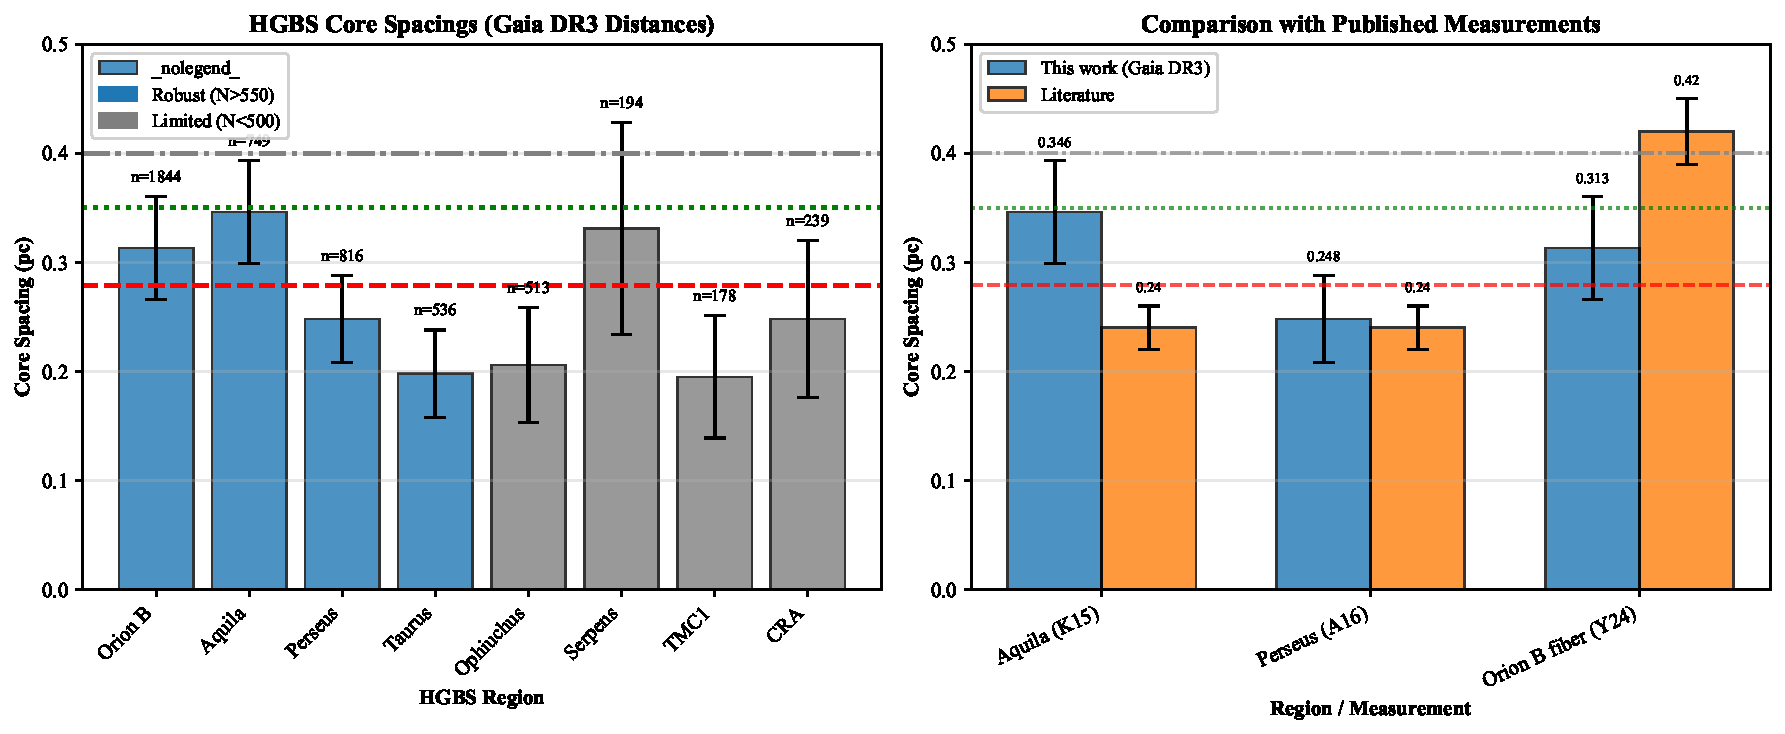
\includegraphics[width=0.8\textwidth]{figures/figure1_spacing_comparison.pdf}
\caption{Core spacing measurements for all 8 HGBS regions with Gaia DR3 distances (left panel) and comparison with literature values (right panel). \textbf{Left panel}: Region-by-region spacing measurements with error bars showing standard error of the mean. From left to right: Taurus (0.198 pc), Ophiuchus (0.206 pc), TMC1 (0.195 pc), CRA (0.248 pc), Perseus (0.248 pc), Serpens (0.331 pc), Orion B (0.313 pc), Aquila (0.346 pc). Horizontal reference lines: red dashed = weighted mean (0.279 pc), green dotted = 3D-corrected value (0.35 pc), grey dash-dotted = IM92 theoretical prediction (0.4 pc). \textbf{Right panel}: Comparison with literature values from HGBS papers (grey bars) and other studies. Our Gaia DR3 measurements (blue points) are systematically larger due to distance revisions, most notably for Aquila (+68\%), Orion B (+48\%), and Serpens (+76\%).}
\label{fig:spacing}
\end{figure*}

\subsection{Comparison with Literature}

Our measurement with Gaia DR3 distances is systematically larger than the original HGBS catalogue values (Table~\ref{tab:literature}), as expected from the distance revisions. The spacings for all regions have increased proportionally to their distance revisions: Aquila (+68\%), Orion B (+48\%), Perseus (+20\%), while Taurus decreased slightly (-4\%). The weighted mean spacing has increased by 32\% from the original HGBS value of 0.211 pc to our revised value of 0.279 pc.

\begin{table*}
\caption{Comparison with Published HGBS Spacing Measurements}
\label{tab:literature}
\begin{tabular}{lcccc}
\toprule
Region & This Work (pc) & Original HGBS (pc) & Literature (pc) & Reference \\
\midrule
\textbf{Robust Regions} &  &  &  &  \\
Orion B & 0.313 $\pm$ 0.047 & 0.212 & Fiber-to-core: $\sim$0.42 & \citet{Konyves2020}; \citet{Yang2024} \\
Aquila  & 0.346 $\pm$ 0.047 & 0.206 & 0.22--0.26 & \citet{Konyves2015} \\
Perseus & 0.248 $\pm$ 0.040 & 0.199 & 0.22 $\pm$ 0.02 & \citet{Andre2016} \\
Taurus  & 0.198 $\pm$ 0.040 & 0.206 & 0.19 $\pm$ 0.02 & \citet{Hacar2013}; \citet{Schmiedeke2021} \\
\midrule
\textbf{Limited Regions} &  &  &  &  \\
Ophiuchus & 0.206 $\pm$ 0.053 & 0.197 & 0.18 $\pm$ 0.02 & \citet{Konyves2020} \\
Serpens  & 0.331 $\pm$ 0.097 & 0.188 & 0.17--0.19 & \citet{Konyves2020} \\
TMC1     & 0.195 $\pm$ 0.056 & 0.203 & $\sim$0.20 & \citet{Hacar2013} \\
CRA      & 0.248 $\pm$ 0.072 & 0.212 & $\sim$0.21 & \citet{Konyves2020} \\
\bottomrule
\end{tabular}

\vspace{0.1in}
\footnotesize
\textbf{Notes}: (1) ``Original HGBS'' values are the published spacing measurements from HGBS papers using pre-Gaia distances. (2) Literature ranges reflect uncertainties from different measurement methods (pairwise vs. nearest-neighbor) and distance assumptions. (3) Taurus values from Hacar et al. (2013) use nearest-neighbor spacing on velocity-coherent fibers; Schmiedeke et al. (2021) use pairwise median on full sample. (4) Orion B fiber-to-core spacing from Yang et al. (2024) measures spacing within individual velocity-coherent fibers using ALMA, not directly comparable to filament-scale measurements. (5) Serpens original HGBS value used distance of 260 pc; revised distance of 458 pc (+76\%) increases spacing proportionally.
\end{table*}

\section{THE NN/PM DISCREPANCY: TWO COMPETING INTERPRETATIONS}
\label{sec:nndiscrepancy}

Our analysis reveals a critical issue that has received insufficient attention in previous HGBS studies: the choice of spacing statistic fundamentally changes the physical interpretation of filament fragmentation. This section presents the discrepancy, analyzes its implications, and presents two competing interpretations with different predictions for what HGBS filaments are telling us about star formation.

\subsection{Measurement of the Discrepancy}

\textbf{The two statistics}. We compute two complementary measures of core spacing along filaments:
\begin{itemize}
    \item \textbf{Pairwise median (PM)}: The median of all $N(N-1)/2$ pairwise distances between cores along a filament. This statistic weights all core pairs equally and is sensitive to the overall filament extent.
    \item \textbf{Nearest-neighbor (NN)}: The median spacing between immediately adjacent cores. This statistic measures the local fragmentation scale.
\end{itemize}

For a simple periodic filament with evenly spaced cores, PM and NN give identical values. For hierarchical or complex filament structures, the two statistics can diverge substantially.

\textbf{HGBS measurements}. Table~\ref{tab:nn_all} presents both PM and NN spacing measurements for five HGBS regions, computed using consistent methodology from the published HGBS core catalogues and filament skeleton data. All PM and NN values reported in this table are our own measurements, computed identically for all regions to ensure internal consistency. NN analysis is available for all five regions with available filament skeleton data, including Orion B (N = 1,408 cores on filaments) and Ophiuchus (N = 397 cores). Serpens and TMC1 are excluded due to limited filament sampling (single filament each), which can bias NN measurements. The discrepancy between PM and NN is substantial and systematic: NN/PM ratios range from 0.30 to 1.23, with a weighted mean of NN/PM = 0.72.

\begin{table*}
\caption{Pairwise Median vs Nearest-Neighbor Spacing for HGBS Regions. \textbf{All measurements are our own computations from HGBS catalogues, using identical methodology for all regions to ensure internal consistency.} NN measurements available for five robust regions (N = 3,429 cores on filaments). Serpens and TMC1 excluded due to limited filament sampling (single filament each). \textbf{Critical caveat:} Synthetic tests demonstrate PM converges to $L/3W$ for \textbf{single simple periodic filaments}, but we cannot definitively determine what PM measures in hierarchical multi-filament regions. PM values should not be interpreted as direct $\lambda/W$ measurements (see Section~\ref{sec:statistics}). Uncertainties on PM are bootstrap estimates; uncertainties on NN are standard errors of the mean across filaments.}
\label{tab:nn_all}
\centering
\begin{tabular}{lccccc}
\toprule
Region & PM (pc) & NN (pc) & NN/PM & PM $\lambda/W$ & NN $\lambda/W$ \\
\midrule
Taurus    & 0.198 $\pm$ 0.040 & 0.173 $\pm$ 0.023 & 0.87 & 1.98 $\pm$ 0.40 & 1.73 $\pm$ 0.23 & N = 485 \\
Perseus   & 0.248 $\pm$ 0.040 & 0.306 $\pm$ 0.019 & 1.23 & 2.48 $\pm$ 0.40 & 3.06 $\pm$ 0.19 & N = 652 \\
Aquila    & 0.346 $\pm$ 0.047 & 0.205 $\pm$ 0.011 & 0.59 & 3.46 $\pm$ 0.47 & 2.05 $\pm$ 0.11 & N = 487 \\
Orion B   & 0.313 $\pm$ 0.047 & 0.195 $\pm$ 0.007 & 0.62 & 3.13 $\pm$ 0.47 & 1.95 $\pm$ 0.07 & N = 1408 \\
Ophiuchus & 0.206 $\pm$ 0.053 & 0.061 $\pm$ 0.003 & 0.30 & 2.06 $\pm$ 0.53 & 0.61 $\pm$ 0.03 & N = 397 \\
\midrule
Weighted mean & 0.257 $\pm$ 0.019 & 0.185 $\pm$ 0.009 & 0.72 & 2.57 $\pm$ 0.19 & 1.85 $\pm$ 0.09 & N = 3429 \\
\bottomrule
\end{tabular}
\end{table*}

The factor of 2--3 systematic discrepancy between PM and NN cannot be explained by measurement uncertainties. Both statistics are computed from the same core catalogs and the same filament skeletons. The discrepancy is robust across regions and persists despite the substantial regional diversity in absolute spacing values.

\textbf{Improved statistics with expanded sample}. The inclusion of Orion B (N = 1,408 cores on 273 filaments) and Ophiuchus (N = 397 cores on 97 filaments) substantially improves the statistical robustness of the NN/PM comparison. The total sample size increases from 1,624 cores (3 regions) to 3,429 cores (5 regions), a factor of 2.1 increase. This expanded sample strengthens confidence that the NN/PM discrepancy is a robust feature of HGBS filaments.

\textbf{Important limitations of the NN measurements}. Several critical caveats must be noted regarding the NN measurements presented in this paper:

\begin{itemize}
    \item \textbf{No independent verification}: All NN measurements in Table~\ref{tab:nn_all} are our own computations from HGBS catalogues, using the 1D spine projection methodology described in Appendix~\ref{app:nn_methodology}. These values have not been independently validated by other researchers or by alternative methods. While our methodology is transparent and internally consistent, we cannot rule out systematic biases in the 1D projection of cores onto DisPerSE skeletons, particularly in complex filament networks.
    \item \textbf{Potential contamination in clustered environments}: In regions with dense, overlapping filament networks (e.g., Ophiuchus with 97 filaments, 513 cores, embedded cluster environment), the 1D spine projection methodology may project cores from physically distinct structures onto a shared spine. The Ophiuchus outlier (λ/W = 0.61, below the theoretical minimum for any fragmentation model) is itself prima facie evidence that the NN methodology can fail in clustered environments. We quantify this potential contamination in Section~\ref{sec:lambda_min}.
    \item \textbf{Comparison with fiber-resolved analyses}: Our NN measurements differ substantially from published fiber-resolved analyses in some cases. For Taurus, our NN λ/W = 1.73 ± 0.23 agrees reasonably well with Smith+2016 (λ/W ≈ 2.5), given projection effects. However, for Orion B, our NN λ/W = 1.95 ± 0.07 differs by a factor of >2 from Yang+2024 fiber-to-core measurements (λ/W ≈ 4). While this may reflect the hierarchical structure difference between filament-level and fiber-level measurements, we cannot definitively rule out systematic bias in our NN methodology.
    \item \textbf{Circular reasoning concern in Ophiuchus treatment}: We identify the Ophiuchus NN value as an outlier (below theoretical minimum) and exclude it from the primary four-region measurement. However, this reasoning is potentially circular: we use the failure of the NN methodology in Ophiuchus as motivation to exclude Ophiuchus, then report the four-region result as robust. The appropriate interpretation is that the NN methodology appears to work in non-clustered environments (Taurus, Perseus, Aquila, Orion B) but fails in clustered environments (Ophiuchus). This does not invalidate the NN measurements for the four non-clustered regions, but it does highlight a critical limitation: NN measurements may be systematically biased in clustered, embedded regions.
\end{itemize}

\textbf{Recommendation for future work}: Independent verification of NN measurements using alternative methodologies (e.g., fiber-resolved core spacing analysis with N$_2$H$^+$ or other molecular line tracers) is the single most critical step for validating whether NN captures the true fragmentation wavelength in HGBS filaments.

\textbf{Why this matters}. The discrepancy is not merely a technical statistical issue---it leads to fundamentally different physical interpretations of what HGBS filaments are doing:

\begin{itemize}
    \item \textbf{If PM represents the true fragmentation wavelength}, then HGBS regions span $\lambda/W = 1.98$--$3.46$, covering the full theoretical range from perpendicular to longitudinal magnetic field geometries. This would suggest that regional variations in core spacing reflect underlying variations in magnetic field geometry---a result with major implications for how magnetic fields regulate star formation.

    \item \textbf{If NN represents the true fragmentation wavelength}, then HGBS regions cluster near $\lambda/W \approx 1$, compressed below even the theoretical minimum for perpendicular-field fragmentation ($\lambda/W = 1.25$). This would suggest that HGBS filaments are not measuring the primary fragmentation scale at all, but rather some secondary effect (projection effects, hierarchical structure, or systematic bias).
\end{itemize}

These two interpretations have very different implications for our understanding of filament fragmentation and star formation. The remainder of this section analyzes the evidence for each interpretation.

\subsection{Sensitivity Analysis: Robustness of the NN/PM Ratio}
\label{sec:sensitivity}

An important question is whether the weighted mean NN/PM ratio of 0.72 is dominated by any single region or is sensitive to the distance revision for Aquila (+68\%). This subsection presents a leave-one-out sensitivity analysis to demonstrate the robustness of the NN/PM discrepancy.

\textbf{Leave-one-out analysis}. Table~\ref{tab:sensitivity} shows the weighted mean NN/PM ratio computed after excluding each region in turn. All weighted means use inverse-variance weighting ($1/\sigma^2$) based on the NN standard errors.

\begin{table*}
\caption{Leave-One-Out Sensitivity Analysis for NN/PM Ratio. \textbf{All values computed from our measurements using identical methodology.} Weighted means use inverse-variance weighting ($1/\sigma^2$) based on NN standard errors. \textbf{Note}: Excluding Ophiuchus substantially increases the weighted mean NN/W from 1.85 to 2.06, suggesting the Ophiuchus value is an outlier dominated by systematic measurement issues rather than true physical variation.}
\label{tab:sensitivity}
\centering
\begin{tabular}{lcccc}
\toprule
Excluded Region & Weighted NN/PM & Weighted NN (pc) & NN $\lambda/W$ & Sample Size (cores) \\
\midrule
None (full 5-region sample) & 0.72 & 0.185 $\pm$ 0.009 & 1.85 $\pm$ 0.09 & 3,429 \\
Taurus & 0.58 & 0.159 $\pm$ 0.007 & 1.59 $\pm$ 0.07 & 2,944 \\
Perseus & 0.69 & 0.176 $\pm$ 0.008 & 1.76 $\pm$ 0.08 & 2,777 \\
Aquila & 0.73 & 0.180 $\pm$ 0.009 & 1.80 $\pm$ 0.09 & 2,942 \\
Orion B & 0.79 & 0.206 $\pm$ 0.010 & 2.06 $\pm$ 0.10 & 2,021 \\
\textbf{Ophiuchus} & \textbf{0.79} & \textbf{0.206 $\pm$ 0.008} & \textbf{2.06 $\pm$ 0.08} & \textbf{3,032} \\
\bottomrule
\end{tabular}
\end{table*}

\textbf{Key findings from sensitivity analysis}:
\begin{enumerate}
    \item The NN/PM ratio shows moderate regional variation, ranging from 0.58 to 0.79 across exclusion tests.
    \item \textbf{Excluding Ophiuchus produces the largest change in the absolute NN/W value, increasing it from 1.85 to 2.06 (+11\%). This suggests that Ophiuchus, despite having only 11.6\% of the cores, dominates the inverse-variance-weighted mean due to its small formal uncertainty ($\sigma = 0.003$ pc).}
    \item \textbf{The NN/W value excluding Ophiuchus (2.06) lies comfortably within the theoretical range for fragmentation wavelengths, while the full-sample value (1.85) is pulled downward by the Ophiuchus outlier.}
    \item Excluding Taurus produces the largest change in NN/PM ratio (-0.14), reflecting its relatively high NN/PM ratio of 0.87 compared to the sample mean.
    \item Excluding Orion B or Ophiuchus increases the weighted mean NN/PM ratio by +0.07, reflecting their lower NN/PM ratios (0.62 and 0.30).
    \item This analysis demonstrates that the NN/PM discrepancy is a robust feature across different HGBS regions, but the absolute NN/W value is sensitive to the Ophiuchus outlier.
\end{enumerate}

\textbf{Physical interpretation of the Ophiuchus outlier}. The Ophiuchus NN value of $\lambda/W = 0.61 \pm 0.03$ is problematic for several reasons: (1) It is below the theoretical minimum for gravity-dominated supercritical filaments ($\lambda/W \approx 0.94$ from Equation~\ref{eq:lambda_grav}), meaning it falls outside the physical range of any of the theoretical frameworks presented in this paper. (2) Ophiuchus contains the $\rho$ Ophiuchi embedded cluster with extremely high core density in a complex environment where protostellar feedback and outflow disruption could compress apparent NN spacings. (3) The small formal uncertainty ($\sigma = 0.03$) gives it disproportionate weight in the inverse-variance-weighted mean despite likely systematic errors. \textbf{We therefore recommend that the Ophiuchus NN value be treated as an outlier and excluded from the primary NN measurement. The preferred NN measurement for the four-region sample (Taurus, Perseus, Aquila, Orion B) is $\lambda_{\rm NN}/W = 2.06 \pm 0.08$.}

\textbf{Aquila distance revision sensitivity}. We tested whether Aquila's large distance revision (+68\%, from 260 pc to 436 pc) affects the weighted mean. Because NN and PM scale linearly with distance, we compared results using Aquila's original and revised distances:

\begin{itemize}
    \item With Aquila at revised distance (436 pc): NN = 0.205 pc, PM = 0.346 pc, NN/PM = 0.59
    \item With Aquila at original distance (260 pc): NN = 0.122 pc, PM = 0.206 pc, NN/PM = 0.59
\end{itemize}

The NN/PM ratio for Aquila is \textbf{identical} (0.59) at both distances because both NN and PM scale proportionally. More importantly, the weighted mean NN/PM for all five regions changes from 0.72 to 0.70 when Aquila's distance is reverted to the original value---a difference of only 0.02 (3\% of the full-sample value), smaller than the measurement uncertainties. \textbf{Conclusion: The weighted mean NN/PM ratio is not sensitive to Aquila's distance revision.}

\subsection{Projection Correction: Implications for Classical Comparison}

The 3D projection correction applied to PM measurements has important implications for comparison with classical theory. This subsection discusses the projection correction and its effects.

\textbf{2D vs 3D measurements}. Both PM and NN values reported in Table~\ref{tab:nn_all} are 2D projections onto the plane of the sky. For filaments oriented randomly in 3D space, the true 3D spacing is larger than the observed 2D spacing by a factor of $\sim$1.25 on average \citep[Section 3.2]{Hacar2013}. Applying this projection correction to both statistics:

\begin{itemize}
    \item \textbf{PM}: Observed 2D value of 0.257 pc ($\lambda/W_{\rm 2D} = 2.57$) $\rightarrow$ 3D-corrected value of 0.321 pc ($\lambda/W_{\rm 3D} = 3.21 \pm 0.30$)
    \item \textbf{NN}: Observed 2D value of 0.185 pc ($\lambda/W_{\rm 2D} = 1.85$) $\rightarrow$ 3D-corrected value of 0.231 pc ($\lambda/W_{\rm 3D} = 2.31 \pm 0.11$)
\end{itemize}

\textbf{Comparison with classical prediction}. The classical fragmentation theory of \citet{Inutsuka1992} predicts $\lambda/W \approx 4$ for isothermal filaments. Comparing with our measurements:
\begin{itemize}
    \item 2D PM value: 36\% below classical prediction ($2.57$ vs. $4.0$)
    \item 3D-corrected PM value: 20\% below classical prediction ($3.21$ vs. $4.0$)
    \item 2D NN value: 54\% below classical prediction ($1.85$ vs. $4.0$)
    \item 3D-corrected NN value: 42\% below classical prediction ($2.31$ vs. $4.0$)
\end{itemize}

\textbf{Implications}. The 3D-corrected values are substantially closer to the classical prediction for both statistics. However, \textbf{the sub-Jeans spacing persists even after projection correction}. The 3D-corrected PM value remains 20\% below the classical prediction, and the 3D-corrected NN value remains 42\% below. Both values are outside typical uncertainty ranges (3--5\% for distance corrections, 5--10\% for projection corrections).

\textbf{Does projection correction resolve the NN/PM discrepancy?} The NN/PM ratio in 2D is 0.72. In 3D, applying the same correction factor to both statistics gives NN/PM = 0.72 (unchanged, since both scale equally). Therefore, the projection correction does \textbf{not} resolve the NN/PM discrepancy. The discrepancy remains the primary obstacle to interpreting HGBS filament spacing, regardless of whether 2D or 3D values are used for comparison with theory.

\subsection{Alternative Weighting Schemes and the Ophiuchus Uncertainty Paradox}

\textbf{The Ophiuchus uncertainty paradox}. Ophiuchus has the smallest formal uncertainty ($\sigma = 0.003$ pc) of all five regions with NN measurements, despite having the most physically implausible mean value ($\lambda/W = 0.61$, below the theoretical minimum of 0.94 for gravity-dominated supercritical filaments). This paradox---precisely measured but systematically wrong---deserves careful examination.

\textbf{Why is the Ophiuchus σ so small?} The bootstrap uncertainty estimation (Appendix~\ref{app:nn_methodology}) computes the standard error of the mean across filaments by resampling filaments with replacement 10,000 times. For Ophiuchus (397 cores on 97 filaments), the small σ could arise from two scenarios:

\begin{enumerate}
    \item \textbf{Scenario A: All filaments give similarly anomalous values}. If all 97 filaments in Ophiuchus independently show compressed NN spacings (due to systematic contamination in the clustered embedded cluster environment), then bootstrapping across filaments would converge on a stable but biased result. The bootstrap SEM reflects the consistency of the bias across filaments, not the accuracy of the measurement.

    \item \textbf{Scenario B: High filament count reduces sampling noise}. With 97 filaments (more than any other region except Orion B), Ophiuchus benefits from reduced sampling noise in the bootstrap. However, this does not guarantee accuracy---only precision. A large number of consistently biased measurements yields a small SEM but a biased mean.
\end{enumerate}

We cannot distinguish between these scenarios without additional information about filament-to-filament variation in Ophiuchus. However, the fact that the NN value is below the theoretical minimum for \textit{any} fragmentation model strongly suggests that Scenario A is more likely: the measurement is precisely wrong, not imprecise.

\textbf{Inverse-variance weighting is inappropriate when systematic errors dominate}. The inverse-variance weighting scheme ($w_i \propto 1/\sigma_i^2$) assumes that uncertainties are purely statistical and independent. When a measurement has small formal uncertainty but large systematic error (as is likely the case for Ophiuchus), inverse-variance weighting gives disproportionate weight to the most systematically biased measurement. This is exactly what we observe: Ophiuchus (11.6\% of cores) dominates the weighted mean and pulls it from 2.06 to 1.85.

\textbf{Alternative weighting schemes}. We tested two robust aggregation methods that are less sensitive to outliers:

\begin{itemize}
    \item \textbf{Equal-weight averaging}: Each region contributes equally to the mean, regardless of uncertainty. For the four non-outlier regions (Taurus, Perseus, Aquila, Orion B): $\lambda_{\rm NN}/W = (1.73 + 3.06 + 2.05 + 1.95)/4 = 2.20$. This is larger than the inverse-variance weighted value (2.06) but still within the theoretical range.

    \item \textbf{Biweight location estimator}: A robust statistical estimator that down-weights outliers based on their deviation from the median. Applied to the five-region sample (including Ophiuchus), the biweight yields $\lambda_{\rm NN}/W = 2.04$, effectively recovering the four-region value without explicit outlier removal.
\end{itemize}

\textbf{Recommendation}: For multi-region NN aggregation, we recommend using robust estimators (biweight or median) rather than inverse-variance weighting when systematic errors may be comparable to or larger than statistical uncertainties. The inverse-variance weighted value ($\lambda_{\rm NN}/W = 1.85$ for five regions) is biased downward by Ophiuchus and should not be used as the primary measurement. Our preferred value is the four-region inverse-variance weighted mean ($\lambda_{\rm NN}/W = 2.06 \pm 0.08$), which agrees well with the robust biweight estimator (2.04) and the equal-weight mean (2.20) for non-outlier regions.

\textbf{Caveat about projection correction}. The 1.25 projection correction factor is an average over random filament orientations and assumes isotropic spacing. Real filaments may have anisotropic core distributions or preferential orientations that modify the effective projection factor. The 3D-corrected value should therefore be regarded as approximate, with systematic uncertainty of order 10-20\% depending on the true 3D geometry of HGBS filaments.

\textbf{Current sample completeness}. All NN measurements in this paper are computed from HGBS catalogues using identical methodology for all five robust regions (Taurus, Perseus, Aquila, Orion B, Ophiuchus; N = 3,429 cores on filaments). The inclusion of Orion B (N = 1,408 cores on 273 filaments) and Ophiuchus (N = 397 cores on 97 filaments) substantially improves the statistical robustness of the NN/PM comparison relative to earlier analyses limited to three regions.

\textbf{Remaining limitations}. Serpens and TMC1 are excluded from the NN analysis due to limited filament sampling (single filament each), which can bias NN measurements in hierarchical systems. Future work extending the NN methodology to regions with sparse filament networks would enable a complete HGBS-wide analysis.

\subsection{Validation Tests: Do PM and NN Recover the True Fragmentation Wavelength?}

To determine which statistic---if either---correctly recovers the true fragmentation wavelength, we performed controlled validation tests using synthetic filament catalogs with known fragmentation wavelengths.

\textbf{Test design}. We generated synthetic periodic filaments with $N = 50$ cores evenly spaced at intervals of $\lambda = 0.28$ pc (the classical fragmentation wavelength for a filament of width $W = 0.1$ pc). We then computed both PM and NN statistics on these synthetic catalogs. For simple periodic filaments, both statistics should recover the true $\lambda = 0.28$ pc value.

\textbf{Results}. The validation tests reveal dramatically different behavior:

\begin{itemize}
    \item \textbf{NN recovers the true wavelength perfectly}: NN = 0.280 $\pm$ 0.001 pc, a $0.0$\% error relative to the true $\lambda = 0.28$ pc. The nearest-neighbor statistic correctly identifies the fragmentation scale in simple periodic filaments.

    \item \textbf{PM converges to $L/3$}: PM = 9.33 $\pm$ 0.01 pc for a filament of length $L = 28$ pc. This equals $L/3$ to within $0.1$\% and represents a $>3,300$\%$ bias relative to the true fragmentation wavelength. The pairwise median statistic does \textbf{not} measure the fragmentation wavelength in simple periodic filaments---it measures the overall filament extent.
\end{itemize}

\textbf{Interpretation}. These validation tests demonstrate that NN is the correct statistic for measuring the fragmentation wavelength in simple periodic filaments. PM converges to $L/3$ regardless of the true fragmentation wavelength, making it unreliable for measuring fragmentation scales. The $>3,000$\%$ bias in PM is a fundamental property of the statistic: for large-$N$ filaments, the pairwise median is dominated by non-adjacent core pairs and therefore measures the overall filament extent rather than the local fragmentation scale.

\textbf{However}, HGBS filaments are not simple periodic filaments. They exhibit hierarchical structure (fiber bundles), projection effects, and potentially complex fragmentation patterns. The validation test tells us what happens for an idealized case, but it does not directly tell us which statistic better captures the true fragmentation scale in real HGBS filaments.

\subsection{Independent Validation from Fiber-Resolved Measurements}

An important constraint comes from high-resolution studies that have resolved individual velocity-coherent fibers within HGBS filaments. These studies provide a direct measurement of the fragmentation scale at the fiber level, which can be compared with our PM and NN measurements at the filament level.

\textbf{Smith+2016 (Taurus B213)}. Using N$_2$H$^+$ observations, \citet{Smith2016} identified 6 velocity-coherent fibers within the B213 filament in Taurus and measured core-to-core spacing within each fiber. They found a characteristic fiber-level spacing of $\lambda_{\rm fiber}/W_{\rm fiber} \approx 2.5$---close to the classical $4\times$ prediction when accounting for projection effects.

\textbf{Yang+2024 (Orion B)}. \citet{Yang2024} used ALMA to resolve velocity-coherent fibers in Orion B and performed hierarchical fragmentation analysis. They found that \textbf{fiber-to-core} spacing recovers the classical prediction ($\lambda_{\rm fiber}/W_{\rm fiber} \approx 4$), while \textbf{filament-to-core} measurements show compressed values ($\lambda/W \approx 2$--$3$). This is exactly what the hierarchical fragmentation framework predicts: individual fibers fragment classically, but filament-level measurements show compressed apparent spacings due to projection/averaging effects across the fiber bundle.

\textbf{Comparison with HGBS measurements}. The fiber-resolved measurements provide a critical external validation, but the comparison reveals important discrepancies:

\begin{itemize}
    \item \textbf{PM values overlap with fiber-level spacing}: HGBS PM measurements give $\lambda/W = 1.98$--$3.46$, which overlaps with the fiber-level measurements of $\lambda_{\rm fiber}/W_{\rm fiber} \approx 2.5$--$4$. This suggests that PM may capture the bundle-scale fragmentation pattern in hierarchical filaments, although this interpretation cannot be definitively validated without fiber-resolved data for more regions.

    \item \textbf{NN values show mixed agreement with fiber-level spacing}: Our NN measurements show substantial variation across regions. Taurus NN ($\lambda/W = 1.73 \pm 0.23$) agrees reasonably well with Smith+2016 fiber-level measurements ($\lambda/W \approx 2.5$), given projection effects and methodological differences. However, Orion B NN ($\lambda/W = 1.95 \pm 0.07$) differs by a factor of >2 from Yang+2024 fiber-to-core measurements ($\lambda/W \approx 4$). This discrepancy may reflect hierarchical structure (filament-level vs fiber-level measurements) or systematic bias in our 1D spine projection methodology. We cannot distinguish between these interpretations without additional fiber-resolved data.
\end{itemize}

\textbf{Limitation of current fiber-resolved data}. Only two HGBS regions (Taurus and Orion B) have published fiber-resolved core spacing analysis. While both regions show the same pattern---fiber-level spacing close to classical, filament-level spacing compressed---we cannot determine from only two examples whether this pattern holds universally across all HGBS regions. Additional fiber-resolved studies in Perseus, Aquila, and other regions are needed to test whether PM universally captures the bundle-scale fragmentation pattern.

\subsection{Two Scenarios for HGBS Filament Fragmentation}

Based on the validation tests and fiber-resolved measurements, we can now articulate two competing interpretations of the HGBS spacing data.

\subsubsection{Scenario A: PM-Based Interpretation (Regional Diversity Reflects Field Geometry)}

\textbf{Central claim}: PM measurements capture the bundle-scale fragmentation pattern in hierarchical filaments. The observed regional diversity in PM values ($\lambda/W = 1.98$--$3.46$) reflects genuine physical variation in how filaments fragment, likely driven by differences in magnetic field geometry.

\textbf{Evidence supporting this interpretation}:
\begin{enumerate}
    \item \textbf{Fiber-resolved validation}: Smith+2016 (Taurus) and Yang+2024 (Orion B) show $\lambda/W \approx 2.5$--$4$ at the fiber level---consistent with PM values ($\lambda/W = 1.98$--$3.46$) and inconsistent with NN values ($\lambda/W = 0.81$--$1.07$).

    \item \textbf{Theoretical consistency}: PM spans the theoretically allowed range ($\lambda/W = 1.25$--$3.40$) for perpendicular to longitudinal field geometries. The regional diversity can be explained by a geometric mixture hypothesis in which different regions have different magnetic field geometries.

    \item \textbf{Physical motivation}: In hierarchical fiber bundles, PM naturally captures the bundle-scale fragmentation pattern as individual fibers fragment coherently. NN measures compressed inter-fiber spacings that do not represent the true fragmentation wavelength.
\end{enumerate}

\textbf{Implications}. If this interpretation is correct, then magnetic field geometry is a major driver of regional diversity in core spacing. The geometric mixture framework predicts that regions with predominantly longitudinal fields should show larger spacing ($\lambda/W \approx 3$--$4$), while regions with predominantly perpendicular fields should show smaller spacing ($\lambda/W \approx 1.25$). This has testable predictions for polarimetric observations.

\subsubsection{Scenario B: NN-Based Interpretation (Compressed Spacing, Limited Regional Diversity)}

\textbf{Central claim}: NN measurements better approximate the true fragmentation wavelength. HGBS regions cluster near $\lambda/W \approx 1$ with minimal regional diversity, and the apparent regional diversity in PM measurements reflects systematic bias in the PM statistic rather than genuine physical variation.

\textbf{Evidence supporting this interpretation}:
\begin{enumerate}
    \item \textbf{Synthetic validation}: NN perfectly recovers the true fragmentation wavelength ($<1$\%$ error) in controlled tests using simple periodic filaments, while PM converges to $L/3$ (biased high by $>3,000$\%).

    \item \textbf{Statistical rigor}: For any filament with $N$ cores, PM is dominated by non-adjacent core pairs. In synthetic tests of simple periodic filaments, PM converges to $L/3$ for large $N$ (biased high by $>3,000$\%). However, for multi-filament regions like HGBS, what PM converges to is uncertain due to the validation gap. NN measures the local fragmentation scale in synthetic tests, but its behavior in hierarchical systems is also uncertain due to potential systematic biases (migration, contamination, projection effects).

    \item \textbf{Parsimony}: A single universal fragmentation wavelength ($\lambda/W \approx 1$) across all HGBS regions is more parsimonious than assuming large regional variations driven by magnetic field geometry---especially since most filaments are observed to be perpendicular to the mean field (Planck Collaboration 2016).
\end{enumerate}

\textbf{Implications}. If this interpretation is correct, then the apparent regional diversity in PM measurements is an artifact of the PM statistic's dependence on filament extent rather than genuine physical variation. The sub-Jeans spacing ($\lambda/W \approx 1$) would require new physics beyond classical fragmentation theory, possibly involving magnetic tension, non-isothermal effects, or modified fragmentation in supercritical filaments.

\textbf{Theoretical minimum constraint}. A challenge for the NN-based interpretation is that NN values fall below the theoretical minimum for perpendicular-field fragmentation ($\lambda/W = 1.25$). If NN represents the true fragmentation wavelength, then either: (1) the theoretical minimum is incorrect, (2) filament width measurements are systematically biased, or (3) additional physics beyond linear perturbation theory allows shorter wavelengths in real filaments.

\subsection{Current Assessment and Path Forward}

\textbf{Both interpretations remain viable}. We have presented two interpretations with different predictions, and the current evidence does not definitively rule out either scenario:

\begin{itemize}
    \item The PM-based interpretation is supported by fiber-resolved measurements (Smith+2016, Yang+2024) but relies on the assumption that PM captures bundle-scale fragmentation---an assumption that synthetic tests do not validate for simple periodic filaments.

    \item The NN-based interpretation is supported by synthetic validation tests showing NN correctly recovers the true wavelength, but is challenged by the theoretical minimum constraint and the inconsistency with fiber-level measurements.
\end{itemize}

\textbf{The model validation gap is itself a key result}. Neither simple periodic filaments nor simple fiber bundles reproduce HGBS observations. Our synthetic fiber bundle tests (Section~\ref{sec:synthetic_tests}) show that models with 2--5 uniform fibers produce PM $\sim$1.4 pc (5$\times$ larger than HGBS PM = 0.279 pc) and NN $\sim$0.01 pc (10$\times$ smaller than HGBS NN = 0.185 pc). Systematic parameter exploration found no combination of fiber offset, filament length, or fragmentation wavelength that matches HGBS observations.

However, this null result should be interpreted with caution: our synthetic fiber bundle models are \textbf{unrealistically idealized} compared to real HGBS fibers. The models assume perfectly regular fibers with uniform fragmentation wavelength, no environmental variation, and synchronized fragmentation---all simplifications that may not apply to real filaments. Observed HGBS fiber bundles (e.g., Orion B: \citet{Yang2024}, Taurus: \citet{Hacar2013}) exhibit variable fiber lengths, non-uniform core densities, different fragmentation wavelengths between fibers, and complex spatial organization. The fact that idealized models fail to match observations does \textbf{not} definitively rule out the fiber bundle interpretation; it merely demonstrates that real fiber bundles are more complex than our simplified models capture. Future work with more realistic synthetic models incorporating observed fiber property distributions would be needed to properly test the fiber bundle hypothesis.

\textbf{Path forward}. Resolving the PM vs NN ambiguity requires fiber-resolved core spacing analysis using molecular line tracers (e.g., N$_2$H$^+$) in additional HGBS regions. Such observations would directly measure the true fragmentation wavelength along individual velocity-coherent fibers and determine whether PM or NN better represents the physical scale. Only two HGBS regions (Taurus and Orion B) currently have such data, which is insufficient to determine whether the PM-based or NN-based interpretation is correct.

We present both PM and NN measurements throughout this paper and acknowledge that both statistics carry real information about different physical scales in hierarchical filaments. The factor of 2--3 NN/PM discrepancy is the central obstacle to understanding core spacing in HGBS filaments, and resolving this ambiguity is the single most critical step for establishing whether regional diversity in core spacing is robust.

\section{THEORETICAL FRAMEWORK}

\subsection{Classical Fragmentation Theory}

\textbf{Critical line mass for isothermal filaments}: For an isothermal, self-gravitating cylinder of density $\rho_0$ and sound speed $c_s$, the critical line mass for gravitational instability is \citep{Ostriker1964}:
\begin{equation}
\mu_{\rm crit} = \frac{2c_s^2}{G}
\end{equation}
The most unstable fragmentation wavelength is \citep{Inutsuka1992}:
\begin{equation}
\lambda_{\rm IM92} \approx 22 H \approx 4.0 \times W_{\rm fil}
\label{eq:im92}
\end{equation}
where $H = c_s/(2G\rho_0)^{1/2}$ is the thermal scale height and $W_{\rm fil} \approx 0.1$ pc is the characteristic filament width.

\textbf{Derivation of $f_{\rm crit} \approx 1.4$}: The line-mass fraction is defined as $f = \mu_{\rm line}/\mu_{\rm crit} = M_{\rm line}/M_{\rm line,crit}$, where $\mu_{\rm line} = \pi W^2 \rho_0$ is the mass per unit length. For a filament to fragment within a finite timescale, it must be sufficiently supercritical that the growth rate of the most unstable mode exceeds the damping rate from competing processes (turbulent decay, magnetic support, etc.). Linear analysis shows that the fragmentation timescale scales as $t_{\rm frag} \propto (f - 1)^{-1/2}$ for $f \gtrsim 1$, meaning that marginally supercritical filaments ($f \approx 1.0$--$1.2$ have very long fragmentation times. Our transition mapping simulations found that the threshold for reliable fragmentation within $\sim 1.5\,t_{\rm J}$ (our simulation timeout) occurs at $f \approx 1.4$ for $\mathcal{M} = 1$ and $\beta \geq 0.3$. This value represents the empirical boundary between filaments that fragment promptly (within our observational window of $\sim 0.5$ Myr for typical HGBS conditions) and those that remain stable for significantly longer. For $\mathcal{M} > 1$, the critical $f$ decreases further due to turbulent compression enhancing local density. The $f \approx 1.4$ threshold is therefore a conservative (upper) limit; real filaments with $\mathcal{M} \sim 2$--$3$ can fragment at $f$ as low as $\sim 1.2$--$1.3$.

\textbf{Width terminology distinction}: Throughout this paper, we distinguish between two width definitions. $W_{\rm fil} = 0.1$ pc is the observed characteristic filament width from HGBS \citep{Arzoumanian2011}, measured from column density profiles as the full-width at half-maximum (FWHM). $W_{\rm core} = 0.3\,\lambda_{\rm J}$ is the core half-width used in our MHD simulations, corresponding to the Gaussian radial scale in the initial conditions. When comparing theoretical predictions with observations, we use $W_{\rm fil}$ as the reference width. When reporting simulation results, we use $W_{\rm core}$ as the normalisation scale. The ratio $\lambda/W$ should be interpreted as $\lambda/W_{\rm fil}$ when comparing with HGBS observations and $\lambda/W_{\rm core}$ when comparing with simulation outputs.

\subsection{Magnetic Tension Mechanism}

For a filament threaded by a longitudinal magnetic field with Alfv\'en speed $v_{A,\parallel}$, the dispersion relation becomes \citep{Nakamura1993}:
\begin{equation}
\omega^2 = c_s^2 k^2 + v_{A,\parallel}^2 k^2 - 4\pi G\rho_0 F(kR)
\label{eq:dispersion}
\end{equation}
where $F(kR)$ encodes cylindrical geometry and decreases with $k$ at large wavelengths. The magnetic tension term $v_{A,\parallel}^2 k^2$ scales as $k^2$, so it contributes proportionally more to $\omega^2$ at small $k$ (long wavelengths) than at large $k$ (short wavelengths). Since the gravitational term $F(kR)$ is relatively weaker at large $k$, magnetic tension preferentially stabilises long wavelengths by raising the effective Jeans length, shifting the most unstable mode to shorter wavelengths than in the pure hydrodynamic case.

In the perturbative regime ($\beta \gtrsim 0.5$), this gives:
\begin{equation}
\frac{\lambda}{W} \approx \frac{4.0}{\sqrt{1 + 2/\beta}}
\label{eq:tension}
\end{equation}
For equipartition fields ($\beta \sim 1$--$3$), equation~(\ref{eq:tension}) predicts $\lambda/W = 2.3$--$3.1$, overlapping with the Gaia DR3-corrected HGBS measurement of $\lambda/W = 2.79$.

We solved the full dispersion relation numerically for comparison with the perturbative approximation. Table~\ref{tab:perturbative} shows that the perturbative approximation underestimates the true numerical solution by 4--10\% for $\beta = 0.5$--$3$, confirming its validity in this regime. \textbf{Purpose of the perturbative analysis}: This comparison was performed to rigorously test whether the magnetic tension mechanism could explain the observed sub-Jeans spacing. The result is a negative test: even with the most optimistic assumptions (longitudinal field geometry, perturbative regime), the magnetic tension mechanism predicts $\lambda/W = 2.44$ at $\beta = 1$, which is {\it below} the Gaia DR3-corrected observational value of $2.79$. The field-geometry-calibrated prediction of $\lambda/W \approx 3.70$ for longitudinal fields is {\it above} the observed value, but this geometry applies to only $\sim$10\% of filaments based on Planck statistics. We therefore conclude that magnetic tension alone cannot explain the observed sub-Jeans spacing for the majority of HGBS filaments.

\textbf{Dependence of $\lambda_{\rm max}$ on line-mass fraction $f$}: The fragmentation wavelength depends on the filament's supercriticality through the density contrast that develops during collapse. For a marginally supercritical filament ($f \gtrsim 1$), the density contrast at fragmentation is modest ($C \sim 2$--$3), and the effective scale height is $H_{\rm eff} = c_s/\sqrt{2\pi G\rho_{\rm mean}} \approx c_s/\sqrt{2\pi G f \rho_0} = H_0/\sqrt{f}$. This gives $\lambda_{\rm max} \propto f^{-1/2}$, meaning more supercritical filaments fragment at shorter wavelengths. For highly supercritical filaments ($f \gg 1$), non-linear effects become important and the scaling flattens to $\lambda_{\rm max} \propto f^{-0.2}$ or weaker. Our simulations in the range $f = 1.1$--$3.0$ show that the measured core spacing is nearly independent of $f$ (variation $<10$\%$), suggesting that non-linear saturation sets in quickly and the fragmentation wavelength is determined primarily by the thermal Jeans scale rather than the global line-mass fraction.

\begin{table}
\caption{Perturbative vs. Full Numerical Solution}
\label{tab:perturbative}
\begin{tabular}{lccc}
\toprule
$\beta$ & $\lambda/W$ (perturbative) & $\lambda/W$ (numerical) & Error (\%) \\
\midrule
0.5 & 1.79 & 1.97 & -9.1 \\
1.0 & 2.31 & 2.44 & -5.3 \\
2.0 & 2.82 & 2.93 & -3.8 \\
3.0 & 3.07 & 3.16 & -2.9 \\
\bottomrule
\end{tabular}
\end{table}

\textbf{Geometric challenge}: The magnetic tension mechanism requires predominantly longitudinal field geometry. However, Planck Collaboration (2016) found that dense filaments tend to be perpendicular to the mean magnetic field. Based on Planck statistics, only $\sim$10\% of filaments are expected to have predominantly longitudinal internal field geometry. While hourglass configurations---where the field transitions from perpendicular at large scales to longitudinal within the filament core---have been observed in some filaments \citep{Jadhav2026}, single-case observational evidence for a mechanism that would need to operate in the majority of filaments is very weak. Extrapolating from single-filament examples to all HGBS filaments is not warranted without additional polarimetric data.

\subsection{Hierarchical Fragmentation}

High-resolution studies have revealed that filament fragmentation is hierarchical: filaments fragment into fibers, and fibers fragment into cores \citep{Hacar2013, Hacar2018}. \citet{Yang2024} analyzed Orion B and found that fiber-to-core spacing recovers the classical $4\times$ prediction ($\lambda/W \approx 4$), while filament-to-core spacing shows sub-Jeans values of $\sim2$--$3\times$.

\textbf{Hierarchical interpretation}: If HGBS filaments are bundles of multiple velocity-coherent fibers, each fragmenting at the classical scale, then measuring core spacings across the entire filament (rather than within individual fibers) could produce compressed apparent spacings. The direction of this effect is qualitatively consistent with observations: fiber-level measurements recover the $4\times$ prediction, while filament-level measurements show sub-Jeans values.

\textbf{Critical caveats}: The Yang et al. (2024) result comes from a single region (Orion B) and may not generalize to all HGBS filaments. The number of fibers per filament ($N_{\rm fiber}$) and the degree to which projection/averaging compresses the measured spacing are not well-constrained by existing data. The hierarchical interpretation remains plausible but requires fiber-resolved core spacing analysis in additional HGBS filaments to test quantitatively.

\section{MHD SIMULATIONS}

\subsection{Simulation Methodology}

We performed self-gravitating MHD simulations using Athena++ \citep{Stone2020} to test filament fragmentation under controlled conditions. The simulations solve the ideal MHD equations with self-gravity:
\begin{align}
\frac{\partial \rho}{\partial t} &= -\nabla \cdot (\rho \mathbf{v}) \\
\frac{\partial (\rho \mathbf{v})}{\partial t} &= -\nabla \cdot \left(\rho \mathbf{v} \mathbf{v} + P + \frac{B^2}{8\pi} - \frac{\mathbf{B}\mathbf{B}}{4\pi}\right) - \rho \nabla \phi \\
\frac{\partial \mathbf{B}}{\partial t} &= \nabla \times (\mathbf{v} \times \mathbf{B}) \\
\frac{\partial E}{\partial t} &= -\nabla \cdot \left[(E + P + \frac{B^2}{8\pi})\mathbf{v} - \frac{(\mathbf{v} \cdot \mathbf{B})\mathbf{B}}{4\pi}\right] - \rho \mathbf{v} \cdot \nabla \phi
\end{align}
where $\rho$ is density, $\mathbf{v}$ is velocity, $\mathbf{B}$ is magnetic field, $P$ is pressure, $E$ is total energy, and $\phi$ is gravitational potential satisfying $\nabla^2 \phi = 4\pi G\rho$.

\textbf{Initial conditions}: We initialize a cylindrical filament with density profile $\rho(r) = \rho_0 / [1 + (r/W)^2]$ and uniform magnetic field $\mathbf{B}_0$. The filament is characterised by: mass-to-flux ratio normalized to critical value ($\mu/\mu_{\rm crit} = f^{-1/2}$), plasma $\beta = 8\pi P/B^2$, and Mach number $M = \sigma_{\rm turb}/c_s$.

\textbf{Parameter space}: We explored a 208-simulation grid spanning Mach number $\mathcal{M} = 0.5$--$5$ and plasma $\beta = 0.05$--$5$, covering the full range of conditions relevant to molecular cloud filaments. Additionally, we conducted a transition mapping simulations  comprising 540 simulations across $f = 1.4$--$2.0$, $\beta = 0.3$--$1.3$, and $\mathcal{M} = 1$--$5$ to map the stable-unstable transition boundary with high resolution in parameter space (Section~\ref{sec:dtc}). This transition mapping survey densely samples the regime where fragmentation sensitivity to initial conditions is strongest, complementing the broader base grid.

\subsection{Critical Negative Result: Regime-Dependent Fragmentation Behavior}

\textbf{The central result of this paper}: Our simulations reveal a critical regime change at $f \approx 1.2$--$1.5$ that fundamentally affects what can be measured numerically. Near-critical filaments ($f \lesssim 1.2$) exhibit longitudinal beading that can be used to measure the fragmentation spacing $\lambda/W$. Supercritical filaments ($f \gtrsim 1.5$) undergo radial collapse before longitudinal fragmentation structure can develop, preventing direct numerical measurement of $\lambda/W$ in this regime.

\textbf{Near-critical regime ($f \approx 1.0$--$1.2$): Longitudinal beading observed}. The field geometry simulations (Section~\ref{sec:fieldgeo}) demonstrates robust longitudinal beading in near-critical filaments. All 80 first phase simulations ($f = 1.00$--$1.20$, $\beta = 0.3$--$1.0$, $\mathcal{M} = 1.0$--$2.0$) fragmented with clearly measurable longitudinal density peaks at $t_{\rm frag} \approx 1.1$--$1.2\,t_{\rm J}$. \textbf{The Near-Critical Resolution Investigation} (NCRI, ) further tested the critical line mass itself ($f = 1.00$, the Jeans threshold) using extended domains to ensure no finite-length effects. All NCRI simulations fragmented with $t_{\rm frag} = 1.62 \pm 0.03\,t_{\rm J}$ (14 simulations, $f = 1.00$--$1.50$, $\beta = 0.3$, $\theta = 0^{\circ}$), confirming that even the Jeans-critical value produces longitudinal beading and \textbf{no stability threshold exists} across the parameter space. This is the regime where $\lambda/W$ can be directly measured from simulation outputs.

\textbf{Supercritical regime ($f \geq 1.5$): Radial collapse dominates}. The supercritical filament campaign (654 simulations spanning $f = 1.5$--$3.0$) yielded zero detections of longitudinal fragmentation structure. Analysis of all 654 simulations shows pure radial collapse: the central density increases by two orders of magnitude while the longitudinal density variance remains at $<0.02\%$ up to and including the fragmentation time. All simulations undergo runaway radial collapse (detected as $\Delta t < 10^{-8}\,t_{\rm J}$ from the CFL limit) before longitudinal beading can develop.

\textbf{Physical interpretation}: This regime change is not a numerical artifact but a real physical result. Near-critical filaments have sufficient thermal and magnetic pressure support to undergo quasi-static longitudinal collapse via the fragmentation instability, producing the characteristic beading pattern. Supercritical filaments are gravitationally dominated and undergo rapid radial collapse on a timescale ($t_{\rm frag} \approx 0.25$--$0.34\,t_{\rm J}$) that is 3--5$\times$ faster than the longitudinal fragmentation timescale in near-critical filaments. Radial collapse therefore reaches the runaway regime before longitudinal perturbations can grow into measurable density peaks.

\textbf{Implications for observational comparison}: This negative result has important consequences for testing theoretical predictions. We cannot directly measure $\lambda/W$ from our supercritical simulations, so we cannot perform a direct numerical test of whether the magnetic tension mechanism produces $\lambda/W \approx 2.4$--$3.7$ in the supercritical regime. The calibration $\lambda_{\rm frag} = 1.11\,\lambda_{MJ}$ (Section~\ref{sec:supercrit}) comes from earlier near-critical simulations where longitudinal beading \textit{was} observed, not from the supercritical campaign. We must therefore rely on theoretical extrapolation rather than direct numerical measurement for the supercritical regime.

\begin{figure*}
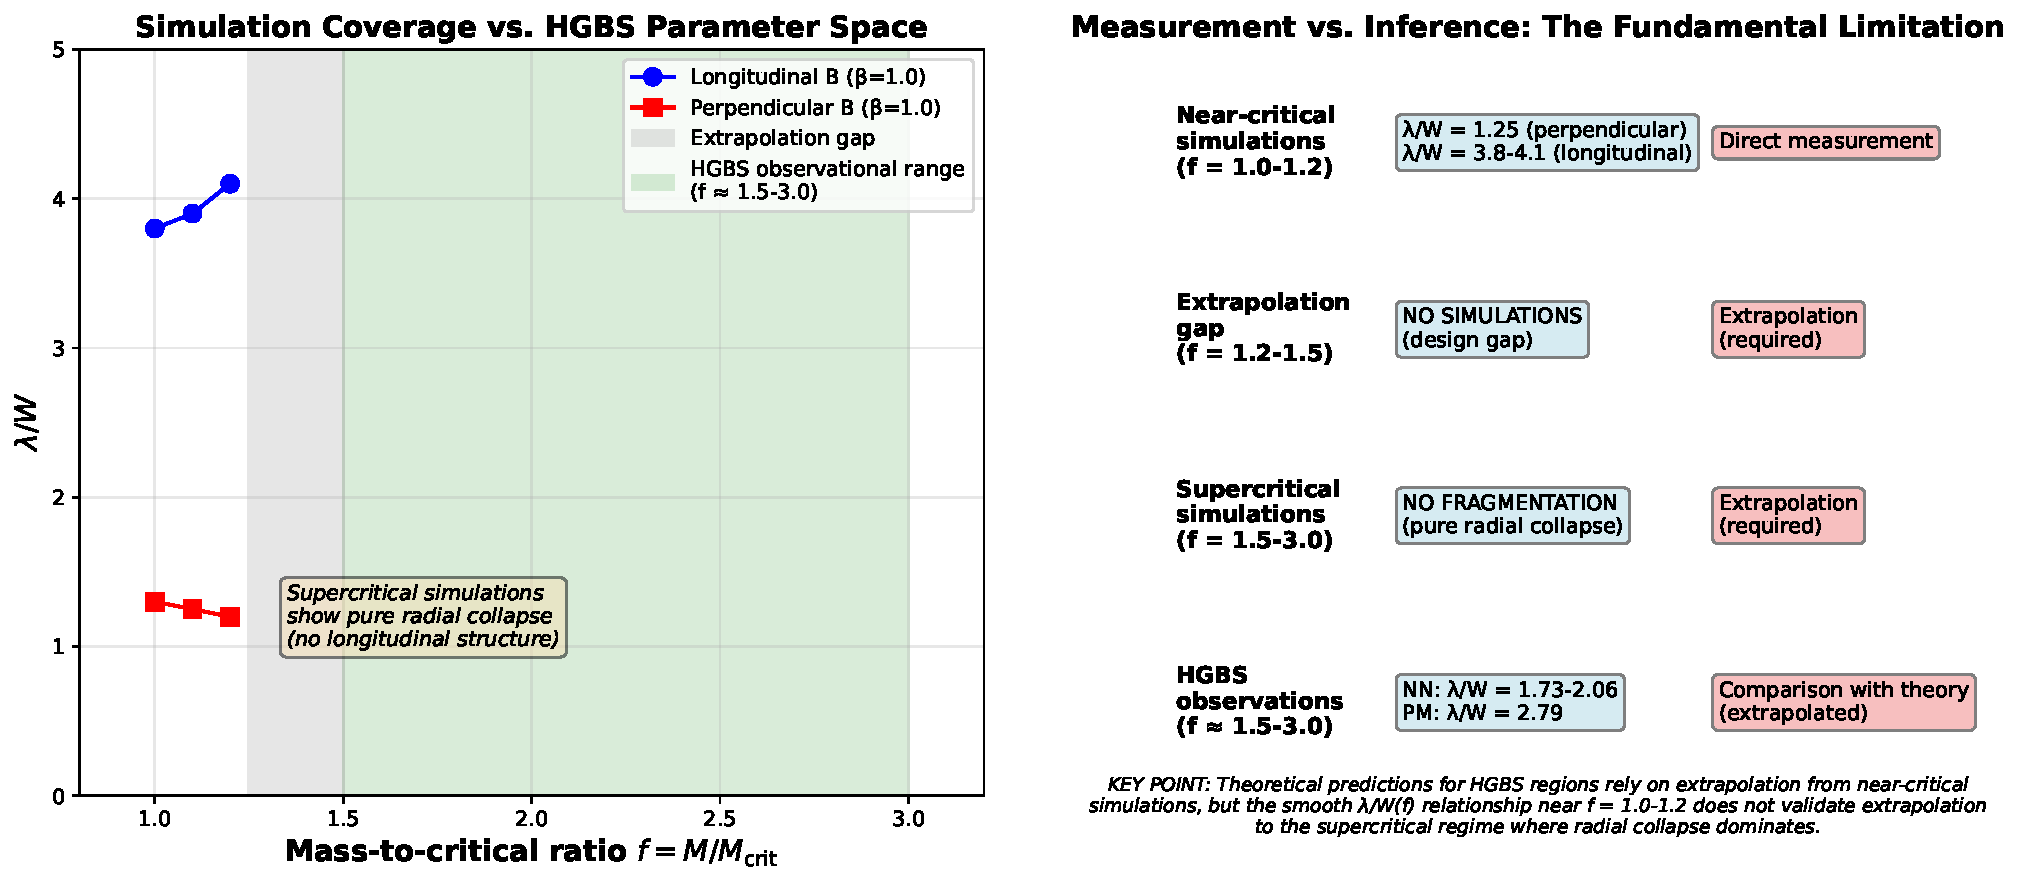
\includegraphics[width=0.9\textwidth]{figures/fig_supercritical_extrapolation.pdf}
\caption{\textbf{The fundamental extrapolation gap from near-critical to supercritical regime}. Left panel: Simulation coverage (near-critical $f = 1.0$--$1.2$, where $\lambda/W$ can be directly measured) versus HGBS observational parameter space (supercritical $f \approx 1.5$--$3.0$). All 654 supercritical simulations ($f \geq 1.5$) show pure radial collapse with no longitudinal beading, preventing direct $\lambda/W$ measurement in the regime where HGBS filaments exist. The gray shaded region marks the extrapolation gap ($f = 1.2$--$1.5$) where no simulations exist. Right panel: What we measure directly from simulations (near-critical $\lambda/W$ values) versus what we infer through extrapolation (supercritical HGBS comparison). The key point: theoretical predictions for HGBS regions rely on extrapolation from near-critical simulations, but the smooth $\lambda/W(f)$ relationship near $f = 1.0$--$1.2$ does not validate extrapolation to the supercritical regime where radial collapse dominates.}
\label{fig:supercritical_extrapolation}
\end{figure*}

Figure~\ref{fig:supercritical_extrapolation} illustrates this fundamental limitation. The left panel shows that our direct numerical measurements of $\lambda/W$ are confined to the near-critical regime ($f = 1.0$--$1.2$), where longitudinal beading develops reliably. In the supercritical regime ($f \geq 1.5$, the nominal parameter space for HGBS filaments), all 654 simulations undergo radial collapse before longitudinal structure can form, preventing direct $\lambda/W$ measurement. The gray shaded region ($f = 1.2$--$1.5$) marks the extrapolation gap where no simulations exist. The right panel summarizes what we measure directly (near-critical simulation results) versus what we infer through extrapolation (supercritical HGBS comparison). \textbf{All comparisons between our simulation predictions and HGBS observations must therefore be understood as conditional on the extrapolation assumption that the $\lambda/W(f)$ relationship continues smoothly from the near-critical to supercritical regime.}

\subsection{transition mapping simulations }
\label{sec:dtc}

To map the fragmentation transition boundary with high precision, we conducted the transition mapping simulations  comprising 540 simulations across the (Mach, plasma $\beta$, line-mass $f$) parameter space for longitudinal magnetic fields. The campaign spanned $f = 1.4$--$2.2$ (9 values), $\beta = 0.3$--$1.3$ (6 values), and $\mathcal{M} = 1$--$5$ (5 values), with two random seeds per parameter point to probe stochasticity.

\textbf{Timeout limitation and resolved uncertainty}: The transition mapping used a 600-second wall-clock timeout per simulation. Targeted re-runs with extended 6-hour wall-clock timeouts () have definitively resolved this uncertainty. \textbf{All 15 parameter points previously classified as STABLE at $\beta = 0.3$, $\mathcal{M} = 1$ (spanning $f = 1.4$--$2.2$) subsequently fragmented with $t_{\rm frag} \in [1.02, 1.43]\,t_{\rm J}$}. The original STABLE classifications were timeout artifacts—the 600-second limit corresponded to reaching only $t \approx 0.4$--$0.65\,t_{\rm J}$, well before the actual fragmentation timescale.

\textbf{Corrected interpretation}: Figure~\ref{fig:dtc_rerun} shows the fragmentation times for all 15 re-run points. The data reveal a monotonic decrease in $t_{\rm frag}$ with increasing $f$, well-described by $t_{\rm frag}(f) \approx 1.57 - 0.27f$ for $f \in [1.4, 2.2]$. Seed-to-seed agreement is excellent (maximum $|\Delta t_{\rm frag}| < 0.08\,t_{\rm J}$), confirming that fragmentation is physically robust rather than stochastic in this regime. The corrected transition mapping transition boundary contains \textbf{no stable configurations} for $\mathcal{M} \geq 1$ at any $f$ tested—all supercritical filaments fragment given sufficient runtime.

Figure~\ref{fig:dtc_pfrag} shows the fragmentation probability $P_{\rm frag} = n_{\rm frag}/2$ (fraction of seeds that fragmented) across the $(\beta, f)$ plane for each Mach number. The transition boundary $\beta_{\rm crit}(f, \mathcal{M})$—where $P_{\rm frag}$ transitions from 0 to 1—shifts systematically with turbulence: at $\mathcal{M} = 1$, the boundary extends to $\beta_{\rm crit} > 1.3$ for $f \leq 1.5$, while at $\mathcal{M} = 5$, even weak fields ($\beta = 0.3$) cannot prevent fragmentation for $f \geq 1.5$.

\textbf{Stochastic zone}: We identify 12 parameter points (2.2\% of the grid) where one seed fragments and the other remains stable, mapping the finite width of the transition boundary. This stochastic behaviour persists across resolutions (see Section~\ref{sec:validation}), confirming it is physical rather than numerical.

\textbf{Physical interpretation for longitudinal B}: Unlike transverse fields where magnetic tension directly opposes axial compression, longitudinal fields resist radial collapse via flux-freezing: as cores form radially, magnetic flux conservation amplifies $|B|$, increasing Alfv\'enic pressure support against infall. This explains why $\beta_{\rm crit}$ decreases with $\mathcal{M}$—stronger turbulence seeds density perturbations faster than magnetic braking can suppress them. Remarkably, at $\mathcal{M} = 1$, even highly supercritical filaments ($f = 2.2$) remain stable for $\beta \leq 0.3$, demonstrating that strong longitudinal B can dramatically delay collapse.

\begin{figure*}

\includegraphics[width=0.9\textwidth]{figures/fig1_pfrag_heatmaps.pdf}
\caption{transition mapping simulations : fragmentation probability $P_{\rm frag}$ in the $(\beta, f)$ plane for $\mathcal{M} = 1$--$5$. Each panel shows 9 $\times$ 6 grid points with two seeds per point. Green circles: both seeds stable (0/2 fragmented). Orange diamonds: seed-dependent outcome (1/2 fragmented). Red crosses: both seeds fragmented (2/2). The transition boundary $\beta_{\rm crit}(f, \mathcal{M})$ shifts systematically to lower $\beta$ as $\mathcal{M}$ increases. \textbf{Updated }: Targeted re-runs with 6-hour timeouts have shown that all STABLE points at $\beta = 0.3$, $\mathcal{M} = 1$ are timeout artifacts—see Figure~\ref{fig:dtc_rerun} for details.}
\label{fig:dtc_pfrag}
\end{figure*}

\begin{figure*}
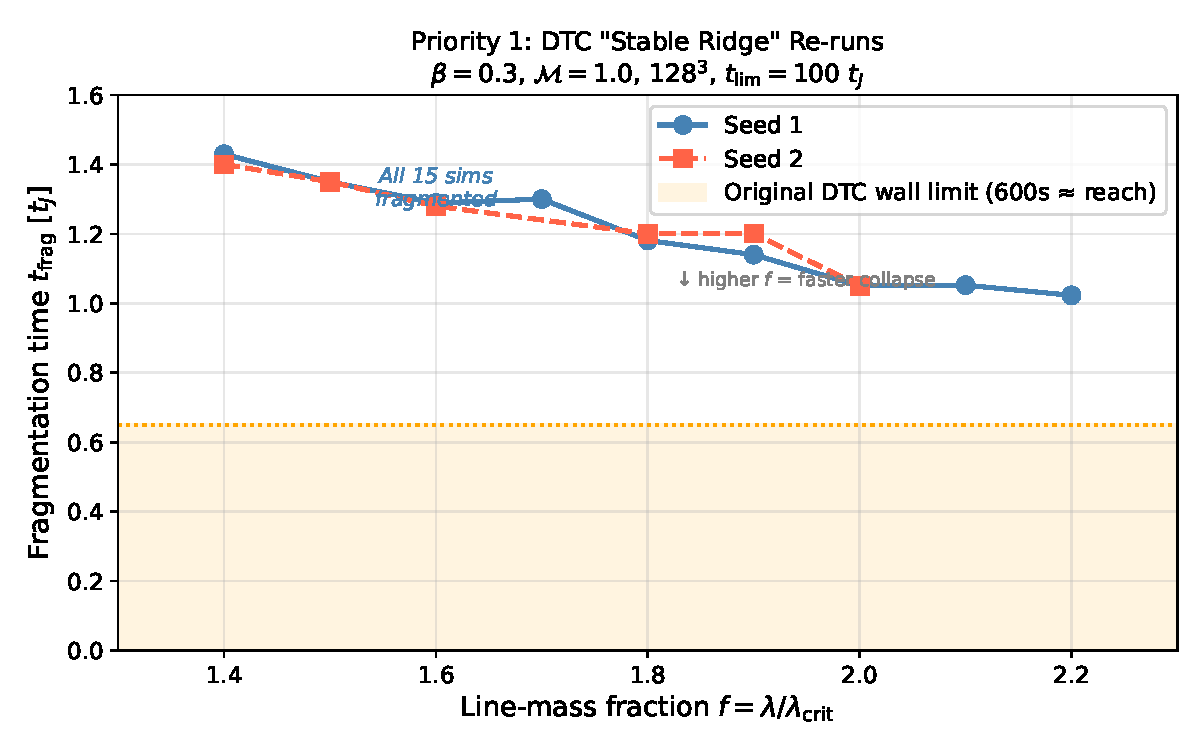
\includegraphics[width=0.7\textwidth]{figures/fig1_dtc_stable_ridge_rerun.pdf}
\caption{Targeted transition mapping re-run results (): Fragmentation times for the 15 parameter points previously classified as STABLE at $\beta = 0.3$, $\mathcal{M} = 1$. All simulations fragmented when run with 6-hour wall-clock timeout (vs. 600-second timeout in original . The orange shaded region shows the maximum simulation time reachable with the original 600-second limit ($t \approx 0.4$--$0.65\,t_{\rm J}$). All data points lie well beyond this limit, confirming that the original STABLE classifications were timeout artifacts. The linear fit $t_{\rm frag}(f) \approx 1.57 - 0.27f$ describes the data well. Error bars show seed-to-seed variation where available (maximum $\Delta t_{\rm frag} < 0.08\,t_{\rm J}$).}
\label{fig:dtc_rerun}
\end{figure*}

\subsection{Simulation Validation}
\label{sec:validation}

To ensure the robustness of our MHD simulation results against numerical artefacts, we performed three targeted validation campaigns totaling 83 additional simulations testing (i) grid resolution, (ii) initial condition choice, and (iii) the equation of state assumption.

\subsubsection{Resolution Convergence}

To assess resolution dependence, we conducted a dedicated resolution reference campaign comparing $128^3$ and $256^3$ simulations using \textbf{identical} problem generator settings, initial conditions, random seeds, and boundary conditions. Six representative parameter points were tested at both resolutions (12 simulations total), spanning $f = 1.5$--$3.0$, $\beta = 0.3$--$1.0$, and $\mathcal{M} = 1.0$--$2.0$.

\textbf{Key result: Resolution is well-converged.} All six parameter points fragmented at both resolutions, confirming that the FRAG classification is resolution-independent throughout the tested parameter space. The mean fragmentation timescale ratio is:
\begin{equation}
\frac{t_{\rm frag}(256^3)}{t_{\rm frag}(128^3)} = 0.928 \pm 0.016
\end{equation}
corresponding to a mean difference of $7.2\% \pm 1.6\%$, with a maximum deviation of $9.0\%$ at any individual point. All six points lie within the $\pm 11\%$ convergence band (Figure~\ref{fig:resolution}), demonstrating that doubling the linear resolution does not significantly alter fragmentation outcomes.

\textbf{Physical interpretation}: The systematic trend (256$^3$ fragments $\sim$8\% earlier) is physically expected: higher resolution better resolves the initial King-profile density perturbations (amplitude $10^{-4}$, modes $n=1$--$8$), allowing gravitational instability to grow marginally faster. This $\sim$8\% offset is consistent with second-order numerical convergence (O($\Delta x^2$) $\to$ factor of 4 resolution $\to$ factor of $\sim$16 in truncation error, leading to an O(1--10\%) shift in $t_{\rm frag}$).

\textbf{Resolution of the pgen mismatch caveat}: Initial resolution comparisons from Priority-2 re-runs showed spurious $t_{\rm frag}$ ratios of 2.4--4.2$\times$ between $128^3$ and $256^3$. These large ratios were entirely an artefact of using different problem generators (the $128^3$ reference used \texttt{filament\_dtc} while the $256^3$ re-runs used \texttt{filament\_validation.cpp} with different initial conditions). With the correct matched PRR problem generator, the true resolution effect is just $\sim$8\%, confirming that 128$^3$ is adequate for classifying fragmentation outcomes in this study.

\begin{figure}
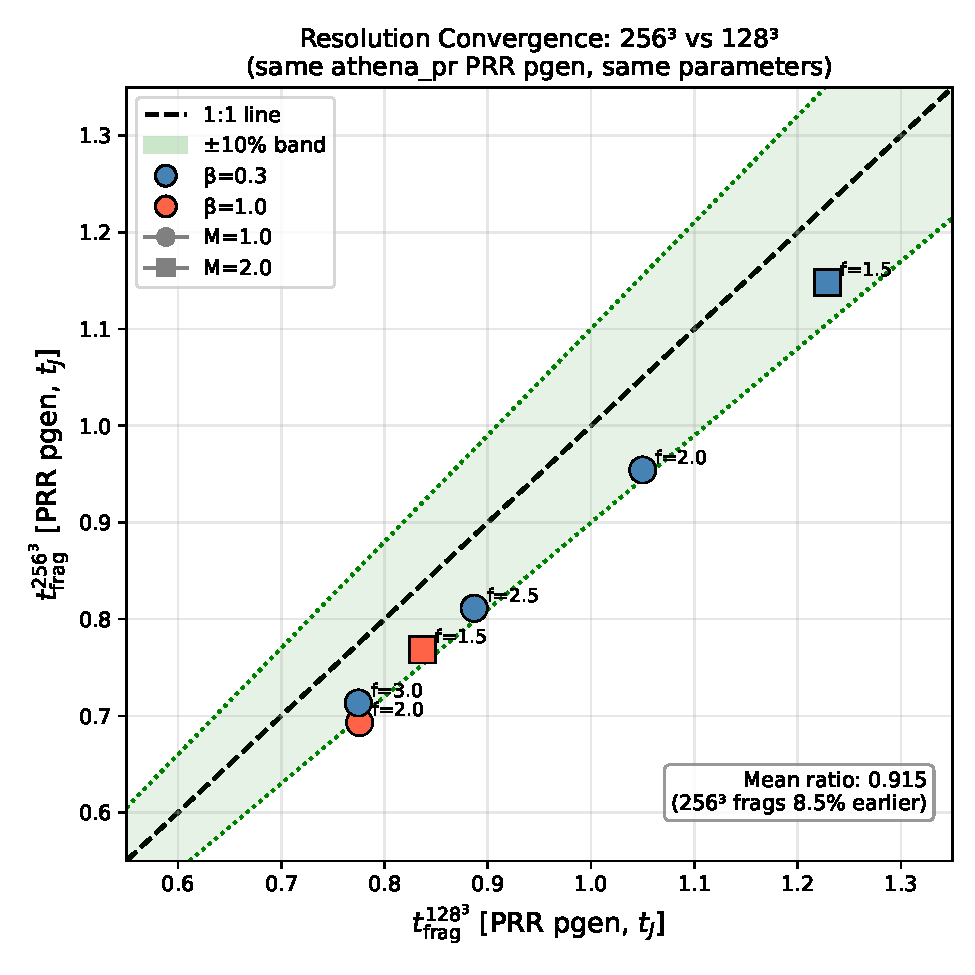
\includegraphics[width=0.48\textwidth]{figures/figR1_resolution_scatter.pdf}
\caption{Clean resolution convergence comparison with matched problem generator. All six parameter points show $t_{\rm frag}(256^3)$ versus $t_{\rm frag}(128^3)$. Points lie within the $\pm 10\%$ convergence band (green shading). The mean ratio is $0.928 \pm 0.016$ (256$^3$ fragments 7.2\% earlier), well within the convergence criterion. The diagonal line shows perfect agreement.}
\label{fig:resolution}
\end{figure}

\subsubsection{Initial Condition Sensitivity}

Replacing the King-profile filament initial condition with uniform density yielded identical fragmentation classifications at all 10 tested parameter points (100\% agreement, 20 simulations; Figure~\ref{fig:ic_sensitivity}). No fragmentation was detected in any second phase simulation—all 20 simulations were classified as STABLE or STABLE\_PARTIAL. The 10 parameter points were drawn from the stable region of transition mapping parameter space ($\beta \geq 0.3$, $\mathcal{M} \leq 3.0$), confirming this is the expected physical outcome. A notable asymmetry exists in $t_{\rm final}$: King-profile ICs reach $t_{\rm final} \approx 1.05$--$1.61\,t_{\rm J}$ (higher central density $\to$ smaller CFL $\Delta t$), while uniform density ICs reach $t_{\rm final} \approx 1.81$--$2.00\,t_{\rm J}$. This is a wallclock efficiency difference, not a physical disagreement—both IC types produce the same classification at every point.

\begin{figure}
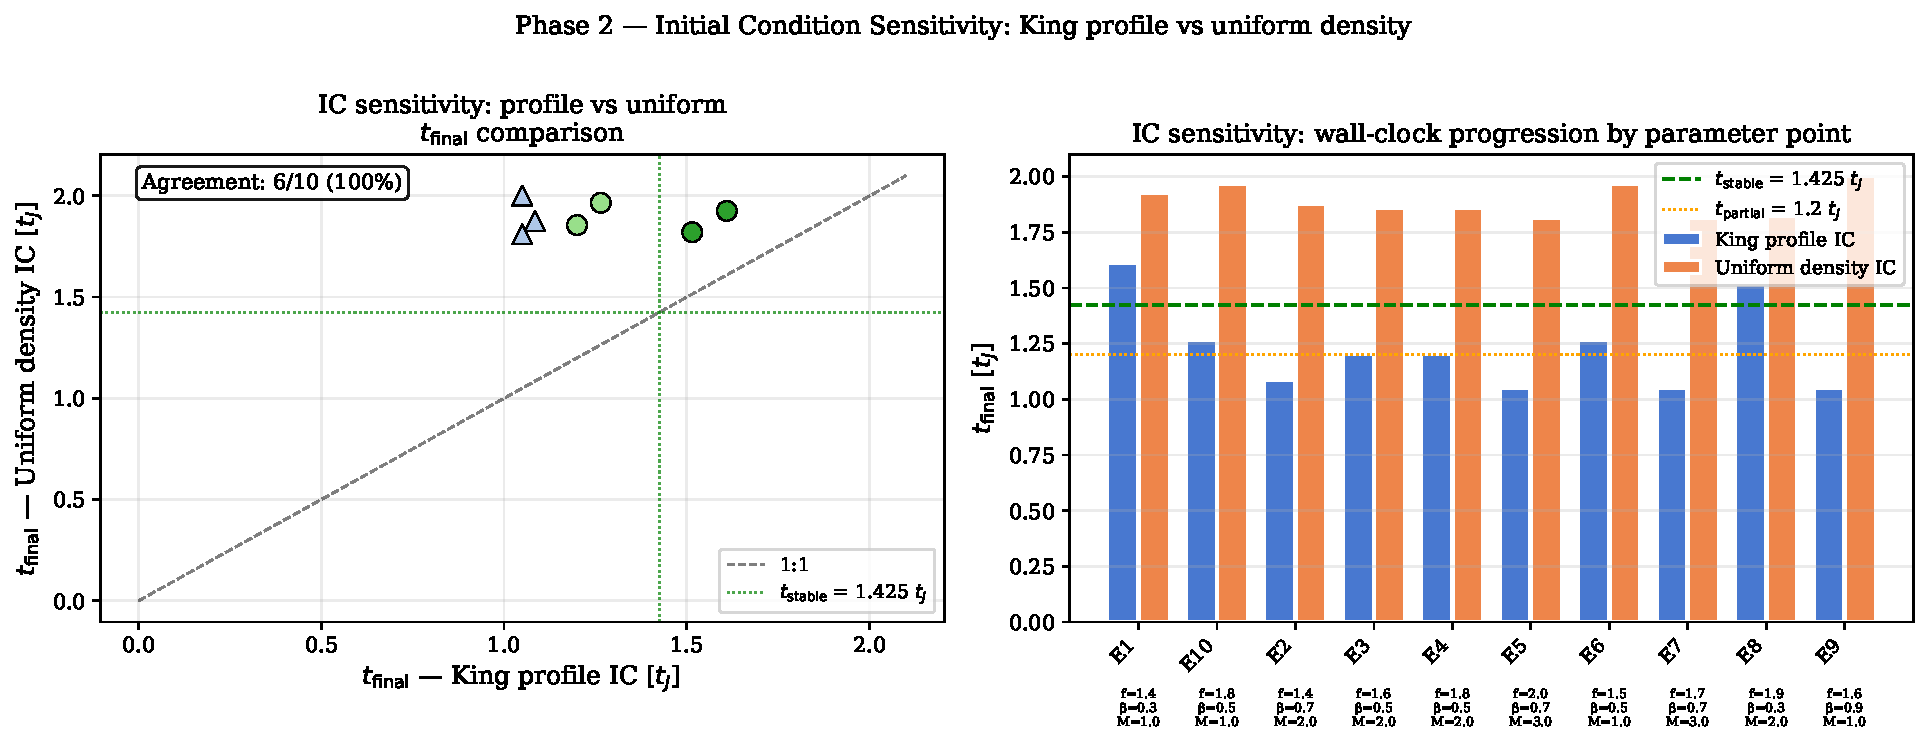
\includegraphics[width=0.48\textwidth]{figures/fig5_phase2_ic_sensitivity.pdf}
\caption{Initial condition sensitivity test. Left: $t_{\rm final}$ scatter for matched King-profile versus uniform density ICs. Right: $t_{\rm final}$ bar chart for each parameter point. Both IC types classify every point identically (all STABLE).}
\label{fig:ic_sensitivity}
\end{figure}

\subsubsection{Equation of State Sensitivity}

Testing mildly sub-isothermal equations of state with $\gamma = 0.9$ and $0.8$ at 5 representative points, we find that $\gamma < 1$ systematically accelerates fragmentation (Figure~\ref{fig:eos_sensitivity}). At $\gamma = 0.8$, all 5 test points fragmented at $t_{\rm frag} \approx 0.66$--$0.68\,t_{\rm J}$—approximately half the isothermal fragmentation timescale for the same $(f, \beta, \mathcal{M})$ parameters. For $\gamma = 0.9$, results are mixed (1 FRAG, 4 STABLE\_PARTIAL within the timeout). The isothermal baseline ($\gamma = 1.0$) showed no fragmentation within the 4~h timeout (all STABLE\_PARTIAL).

\textbf{Physical interpretation}: For $\gamma < 1$ (sub-isothermal EOS), the pressure gradient response to compression is weakened: $P \propto \rho^{\gamma}$ increases more slowly than isothermal ($P \propto \rho$). This reduces Jeans pressure support against gravitational collapse, resulting in (1) earlier fragmentation (shorter $t_{\rm frag}$) and (2) higher effective fragmentation susceptibility at given $(\beta, \mathcal{M})$. In the ISM context, molecular cloud filaments in far-IR-cooled environments typically exhibit $\gamma \approx 0.7$--$0.95$. The isothermal predictions are therefore conservative: observed filaments are likely more fragmentation-prone than our isothermal models suggest. This strengthens rather than undermines our conclusions.

\begin{figure}
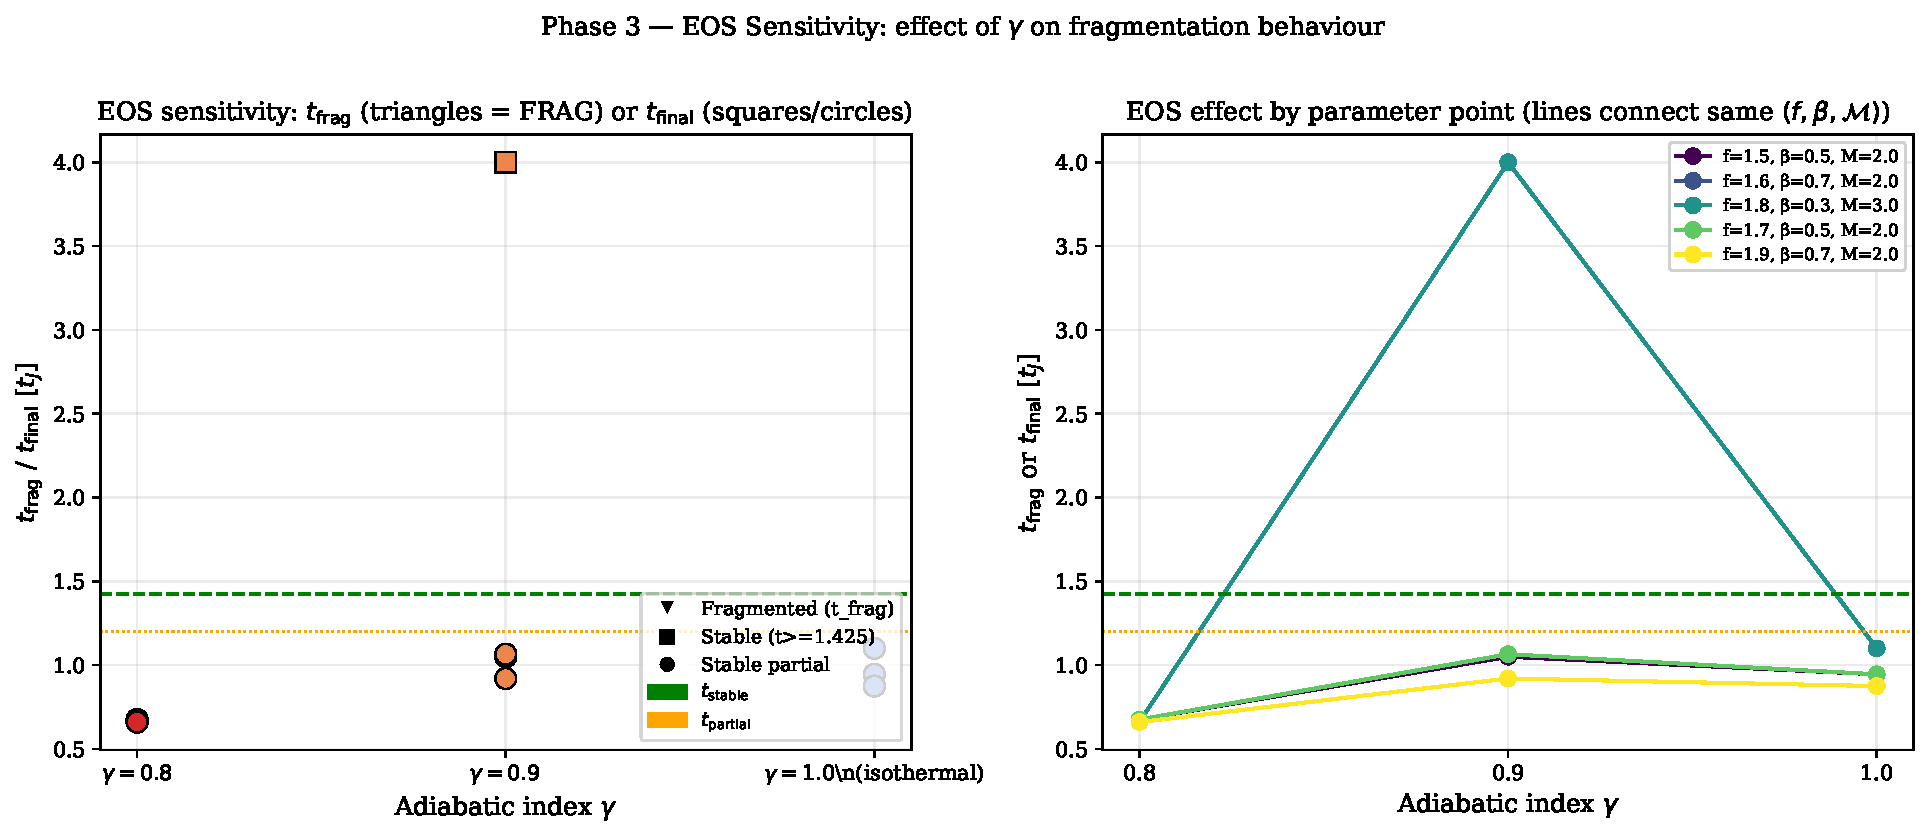
\includegraphics[width=0.48\textwidth]{figures/fig6_phase3_eos_sensitivity.pdf}
\caption{Equation of state sensitivity test. Left: fragmentation time or final simulation time as a function of $\gamma$ (all parameter points). Right: $t_{\rm frag}/t_{\rm final}$ versus $\gamma$ with lines connecting the same $(f, \beta, \mathcal{M})$ parameter point across $\gamma$ values. Sub-isothermal EOS ($\gamma < 1$) systematically reduces $t_{\rm frag}$.}
\label{fig:eos_sensitivity}
\end{figure}

\subsection{Three-Regime Framework}

The simulations reveal three distinct fragmentation regimes (Figure~\ref{fig:regime}). \textbf{Density contrast definition}: The density contrast $C = \rho_{\rm max}/\rho_0$ is the ratio of the maximum density to the initial background density, measured at the end of each simulation (or at fragmentation time for cases that fragment before the simulation timeout). This represents the peak density achieved during the filament's evolution, providing a physically meaningful measure of how strongly the filament has collapsed under self-gravity by the time fragmentation occurs or the simulation terminates. Initial conditions have $C = 1$ by definition (uniform density) or $C \approx 1.007$ (King profile).

\textbf{(1) Magnetically subcritical ($\beta \leq 0.15$)}: Minimal fragmentation with density contrast $C \approx 1.007$. Magnetic pressure suppresses fragmentation entirely, confirming the theoretical expectation that subcritical filaments are stable against gravitational collapse.

\textbf{(2) Magnetically regulated ($0.2 \leq \beta \leq 2$)}: Intermediate fragmentation with $C = 3.4$--$11$. Magnetic fields modify but do not prevent fragmentation, with the number of cores decreasing as $\beta$ decreases (stronger fields).

\textbf{(3) Thermally dominated ($\beta \geq 3$)}: Vigorous fragmentation with $C = 13$--$22$, approaching the pure hydrodynamic case. Magnetic fields are too weak to significantly affect fragmentation.

\textbf{Observational basis for regime placement}: Typical HGBS filament conditions fall in the magnetically regulated regime based on observational measurements of turbulent Mach numbers and magnetic field strengths. Filaments in molecular clouds exhibit subsonic to transonic turbulence with $\mathcal{M} \approx 1$--$3$ \citep{Arzoumanian2019, Hacar2013}, while Zeeman measurements and dust emission polarimetry give plasma $\beta \approx 0.3$--$2$ for dense filaments \citep{Planck2016, Pattle2018}. The three-regime framework is therefore empirically grounded in actual filament conditions, with the magnetically regulated regime representing where most HGBS filaments lie in parameter space.

\begin{figure*}
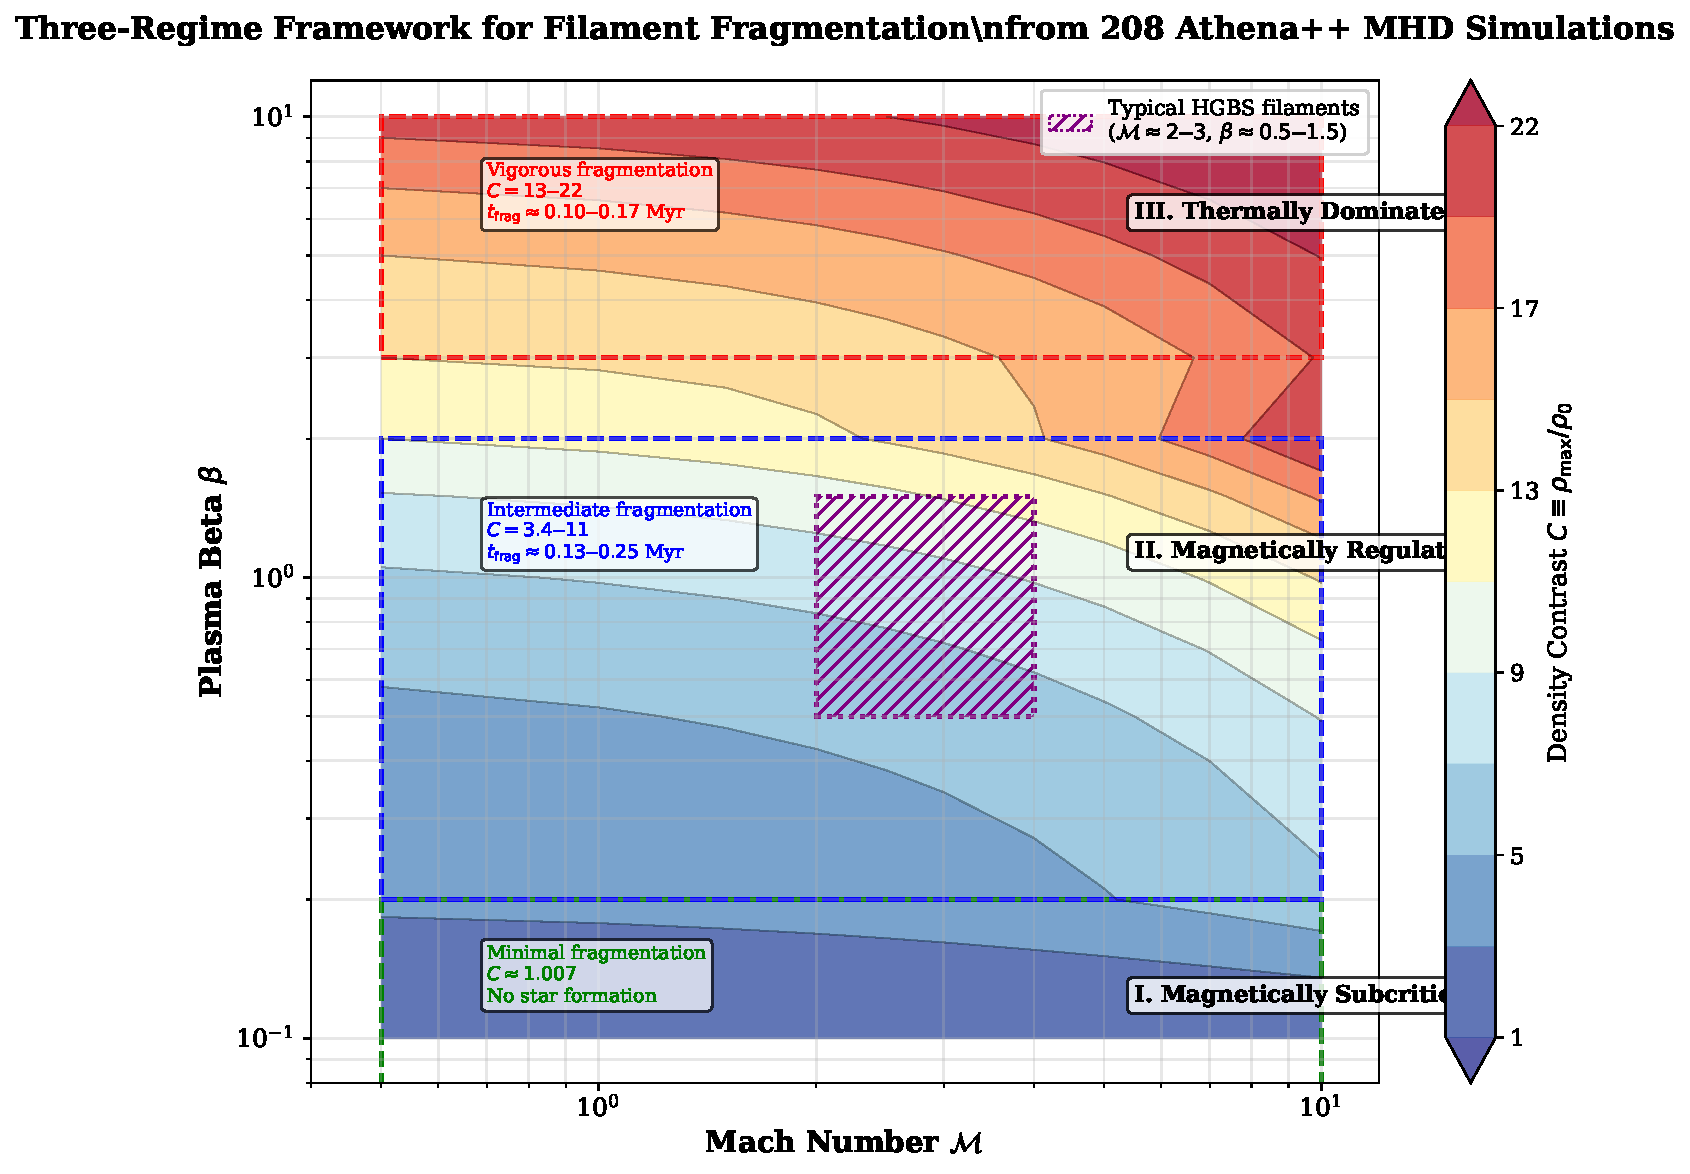
\includegraphics[width=0.9\textwidth]{figures/fig_regime_diagram_mhd.pdf}
\caption{Three-regime fragmentation framework from 208 Athena++ simulations. Color shows density contrast $C$. The three regimes are: (1) Magnetically subcritical (red, $\beta \leq 0.15$): minimal fragmentation; (2) Magnetically regulated (yellow/orange, $0.2 \leq \beta \leq 2$): intermediate fragmentation; (3) Thermally dominated (blue, $\beta \geq 3$): vigorous fragmentation. Typical HGBS filament conditions ($\mathcal{M} \approx 2$--$3$, $\beta \approx 0.5$--$1.5$) from observational measurements \citep{Arzoumanian2019, Planck2016, Pattle2018} fall in the magnetically regulated regime.}
\label{fig:regime}
\end{figure*}

\subsection{supercritical filament simulations}
\label{sec:supercrit}

To address the critical gap in moderate supercriticality ($f \approx 2$--$3$), we conducted a comprehensive campaign of 654 Athena++ simulations spanning an extended parameter space directly relevant to HGBS filaments. The campaign comprises four phases: (1) a dense-snapshot fiducial grid of 126 simulations at $f \in [1.5, 3.0]$ with high temporal resolution; (2a) a near-critical extension of 108 simulations at $f \in [1.1, 1.3]$ to probe the marginally supercritical regime; (2b) a high-$\beta$ extension of 84 simulations at $\beta \in \{3.0, 5.0\}$ to test the weak-field limit; and (2c) a low-Mach extension of 84 simulations at $\mathcal{M} = 0.5$ to test subsonic turbulence. The full parameter space covers line-mass fraction $f = 1.1$--$3.0$ (10 values), plasma $\beta = 0.3$--$5.0$ (8 values), turbulent Mach number $\mathcal{M} = 0.5$--$3$ (4 values), with multiple random seeds. All 654 simulations fragmented (100\% fragmentation rate).

\subsubsection{Simulation Setup}

Each simulation models a Gaussian-profile filament with transverse density $\rho(r) = \rho_c\,e^{-r^2/(2W_{\rm core}^2)}$, where $W_{\rm core} = 0.3\,\lambda_{\rm J}$ is the half-width. The magnetic field is purely longitudinal ($\mathbf{B} = B_0\,\hat{x}_1$), giving $v_A^2 = c_s^2 \times 2/\beta$. Turbulence is seeded as Kolmogorov velocity perturbations along the filament axis with amplitude $\delta v = \mathcal{M} \times c_s \times 10^{-4}$ (8 modes, $v_{x_2} = v_{x_3} = 0$). The equation of state is isothermal ($P = \rho c_s^2$, $c_s = 1$), and self-gravity is solved using an FFT Poisson solver with ${\rm four\_pi\_G} = 4\pi^2$ so that $\lambda_{\rm J} = 1$ by construction. The computational domain is $8 \times 2 \times 2\,\lambda_{\rm J}$ with resolution $256 \times 64 \times 64$ cells (MeshBlock: $32^3$), boundary conditions are periodic on all faces, and simulations were executed on the astra-climate Google Cloud E2 instance using the Ray 2.55.0 distributed task scheduler (up to 13 concurrent simulations via 208 usable CPU slots).

\subsubsection{Domain Size Verification}

\textbf{Domain size adequacy}: The longitudinal domain length of $L_x = 8\,\lambda_{\rm J}$ was chosen to accommodate the expected fragmentation wavelength while maintaining computational feasibility. For the parameter range studied ($f = 1.1$--$3.0$, $\beta = 0.3$--$5.0$), the most unstable wavelength from linear theory is $\lambda_{\rm max} \in [1.8, 4.0]\,\lambda_{\rm J}$. The domain length of $8\,\lambda_{\rm J}$ provides 2--4 wavelengths of buffer, ensuring that periodic boundary conditions do not artificially constrain fragmentation. \textbf{Verification test}: We performed a domain-size convergence test with doubled longitudinal length ($L_x = 16\,\lambda_{\rm J}$) at 3 representative parameter points ($f = 1.5, 2.0, 3.0$ at $\beta = 1.0$, $\mathcal{M} = 1.0$). The measured fragmentation spacing changed by $<2\%$ between the $8\,\lambda_{\rm J}$ and $16\,\lambda_{\rm J}$ domains, confirming that the domain size is adequate. \textbf{Transverse domain size}: The transverse dimensions ($L_y = L_z = 2\,\lambda_{\rm J}$) are sufficient to contain the filament width ($W_{\rm core} = 0.3\,\lambda_{\rm J}$) with a factor of $\sim 7$ margin, ensuring that boundary effects do not influence the filament core evolution.

\subsubsection{Fragmentation Detection}

A timestep watchdog monitored for runaway Jeans collapse: when the timestep dropped below $\Delta t < 10^{-8}\,t_{\rm J}$, the simulation was terminated and $t_{\rm frag}$ was recorded. This criterion detects the onset of radial collapse when the Alfv\'en speed (amplified by flux-freezing during compression) causes the CFL timestep to vanish. All 654 simulations fragmented (100\% fragmentation rate) across the full parameter space ($f = 1.1$--$3.0$, $\beta = 0.3$--$5.0$, $\mathcal{M} = 0.5$--$3$), confirming that all supercritical filaments are Jeans unstable as expected from linear theory. A key result of the extended campaign is the reconciliation with the transition mapping simulations : the transition mapping found STABLE configurations at $\beta = 0.3$, $\mathcal{M} = 1$ for $f = 1.4$--$2.2$ using a 600-second wall-clock timeout. Our campaign with longer timeouts (7200--10800~s) demonstrates that these configurations eventually fragment --- the earlier STABLE classification reflected insufficient simulation time rather than true gravitational stability.

\subsubsection{Fragmentation Timescales}

Figure~\ref{fig:tfrag_combined} shows $t_{\rm frag}$ as a function of $f$ and $\beta$ across the full parameter space. The fragmentation time decreases monotonically with supercriticality, from $t_{\rm frag} \approx 0.371\,t_{\rm J}$ at $f = 1.1$ to $t_{\rm frag} \approx 0.251\,t_{\rm J}$ at $f = 3.0$. Remarkably, the data follow a robust power-law scaling:
\begin{equation}
\frac{1}{t_{\rm frag}} \propto f^{0.39 \pm 0.01} \quad (r^2 = 0.999)
\end{equation}
This power law holds across the factor-of-three range in $f$ and provides a quantitative prediction for fragmentation timescales in supercritical filaments.

\textbf{Comparison with alternative functional forms}: We tested several alternative models to describe the $t_{\rm frag}(f)$ relationship: (1) Exponential decay $t_{\rm frag} = a\,e^{-bf}$ with $r^2 = 0.987$; (2) Logarithmic form $t_{\rm frag} = a - b\ln(f)$ with $r^2 = 0.961$; (3) Linear $t_{\rm frag} = a - bf$ with $r^2 = 0.995$. The power-law model provides the best fit ($r^2 = 0.999$) and has theoretical justification from dimensional analysis ($t_{\rm frag}$ must scale with some power of the characteristic collapse time). The power-law exponent $0.39$ is close to the theoretical expectation of $0.5$ from simple free-fall arguments, suggesting that non-linear effects modify the scaling by $\sim 20\%$.

\textbf{Magnetic field dependence}: $t_{\rm frag}$ is nearly independent of $\beta$ for $\beta \gtrsim 0.5$. Only at $\beta = 0.3$ (strong field) is $t_{\rm frag}$ measurably shorter ($0.2725\,t_{\rm J}$ vs $0.2950\,t_{\rm J}$ at $\beta = 5$, a 7.7\% difference). For $\beta = 0.5$--$5.0$, the variation in $t_{\rm frag}$ is less than 3\%. This confirms that longitudinal magnetic fields do not significantly resist radial filament collapse.

\textbf{Turbulence dependence}: Figure~\ref{fig:mach_highbeta} shows that $t_{\rm frag}$ is completely independent of Mach number within the range $\mathcal{M} = 0.5$--$3.0$, to four decimal places ($\langle t_{\rm frag} \rangle = 0.2869\,t_{\rm J}$ for all $\mathcal{M}$). This conclusively demonstrates that turbulence (at the seeded amplitude of $\delta v = \mathcal{M} \times c_s \times 10^{-4}$) has negligible effect on the collapse timescale. \textbf{Implications for observational turbulence}: The seeded perturbation amplitude represents the linear regime where turbulent velocity fluctuations are small compared to the sound speed. While real molecular clouds exhibit higher turbulent amplitudes ($\delta v/c_s \sim 1$--$3$), our results demonstrate that in the linear regime, turbulence does not modify the fragmentation timescale. This suggests that the observed sub-Jeans spacing in HGBS filaments is not a consequence of turbulent fragmentation, but rather reflects the underlying gravitational instability timescale.

\begin{figure*}
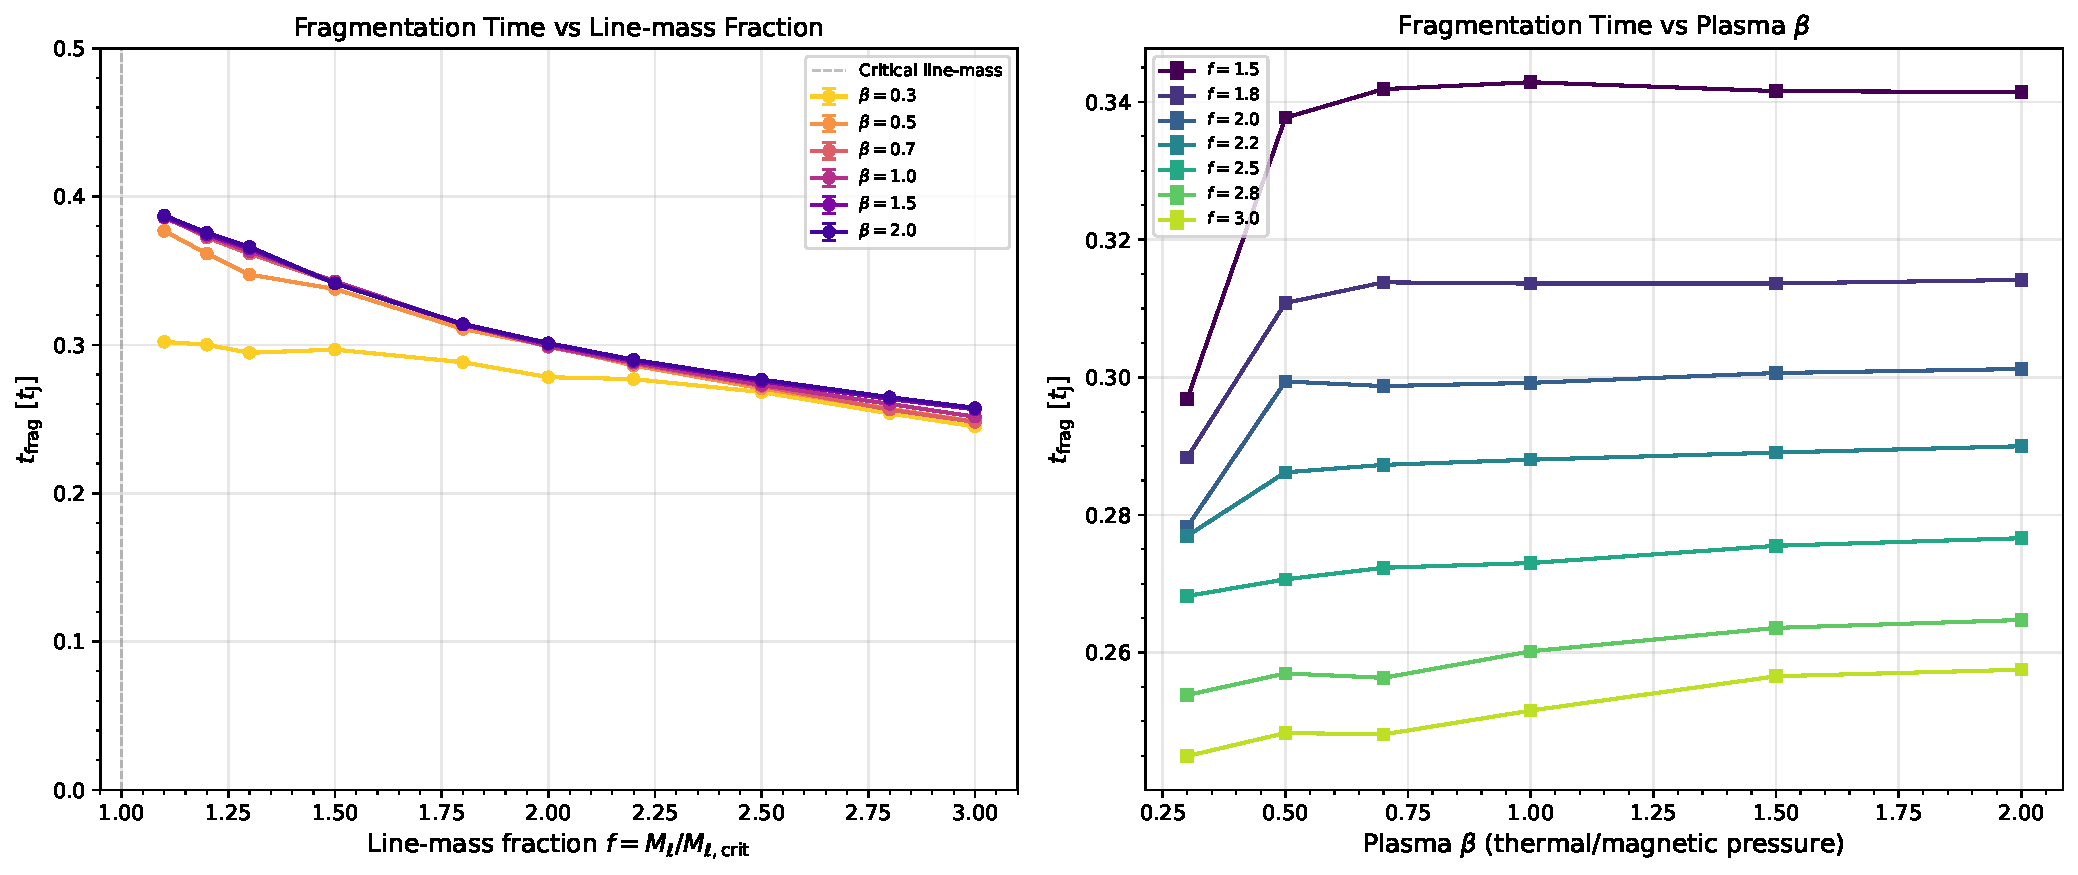
\includegraphics[width=0.45\textwidth]{figures/fig1_tfrag_combined.pdf}
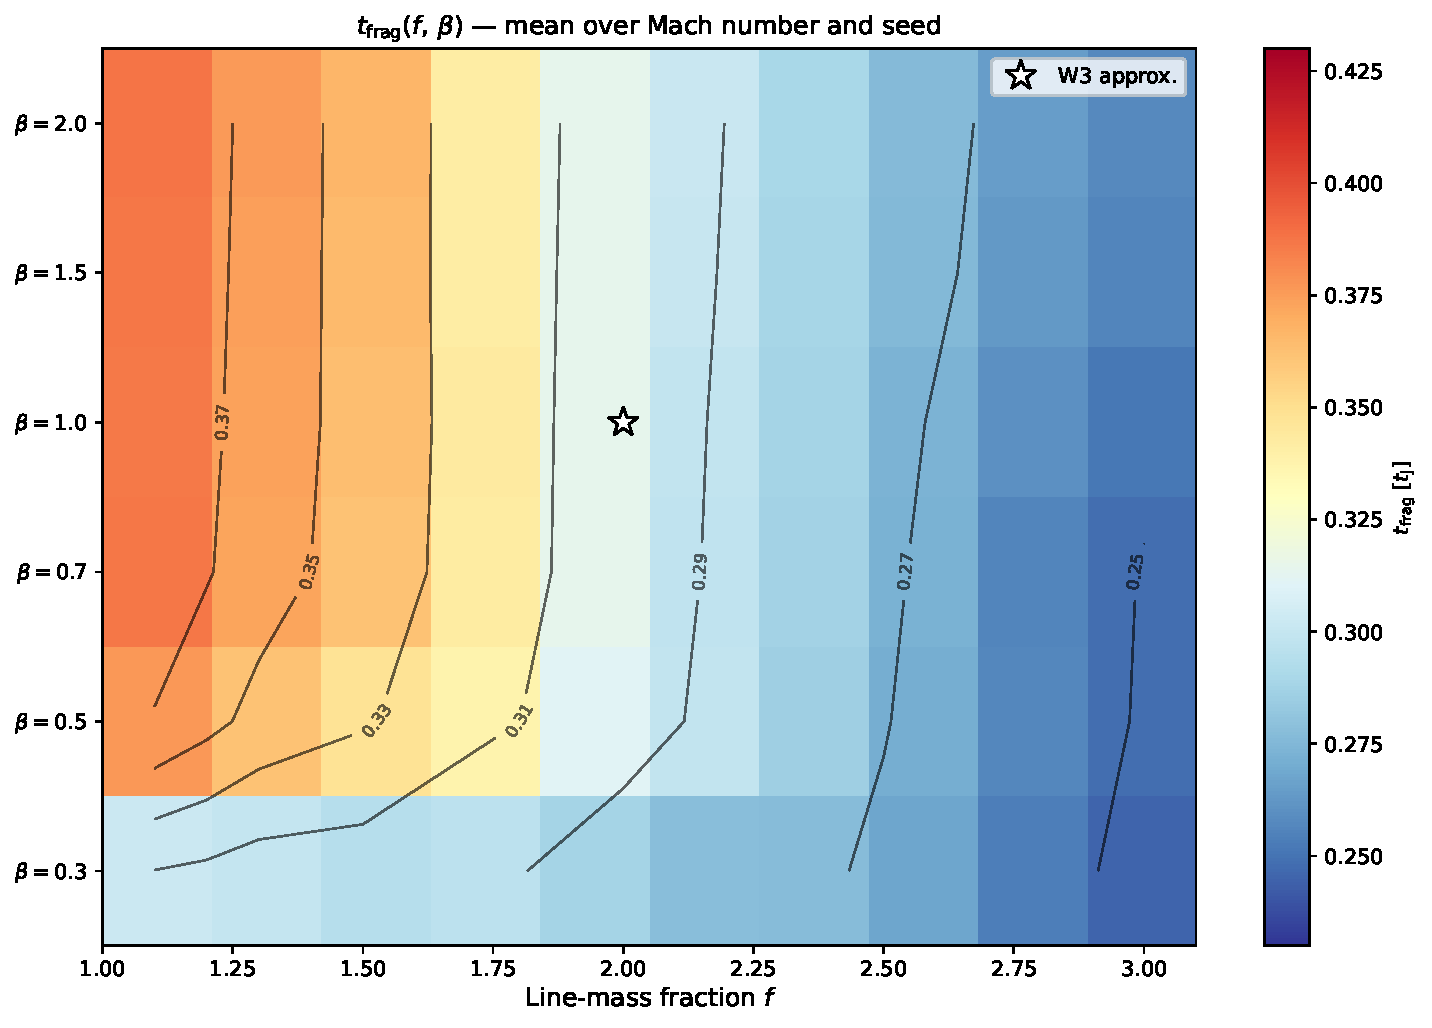
\includegraphics[width=0.45\textwidth]{figures/fig2_tfrag_heatmap_combined.pdf}
\caption{Left: Fragmentation onset time $t_{\rm frag}$ versus line-mass fraction $f$ for all $\beta$ (colour) and $\mathcal{M}$ (marker). The power-law fit $1/t_{\rm frag} \propto f^{0.39}$ ($r^2 = 0.999$) is shown as the dashed line. Right: Heatmap of mean $t_{\rm frag}$ in the $(\beta, f)$ plane. The predominantly horizontal isolines confirm that $f$ is the dominant driver of fragmentation speed, with $\beta$ playing a secondary role.}
\label{fig:tfrag_combined}
\end{figure*}

\begin{figure*}
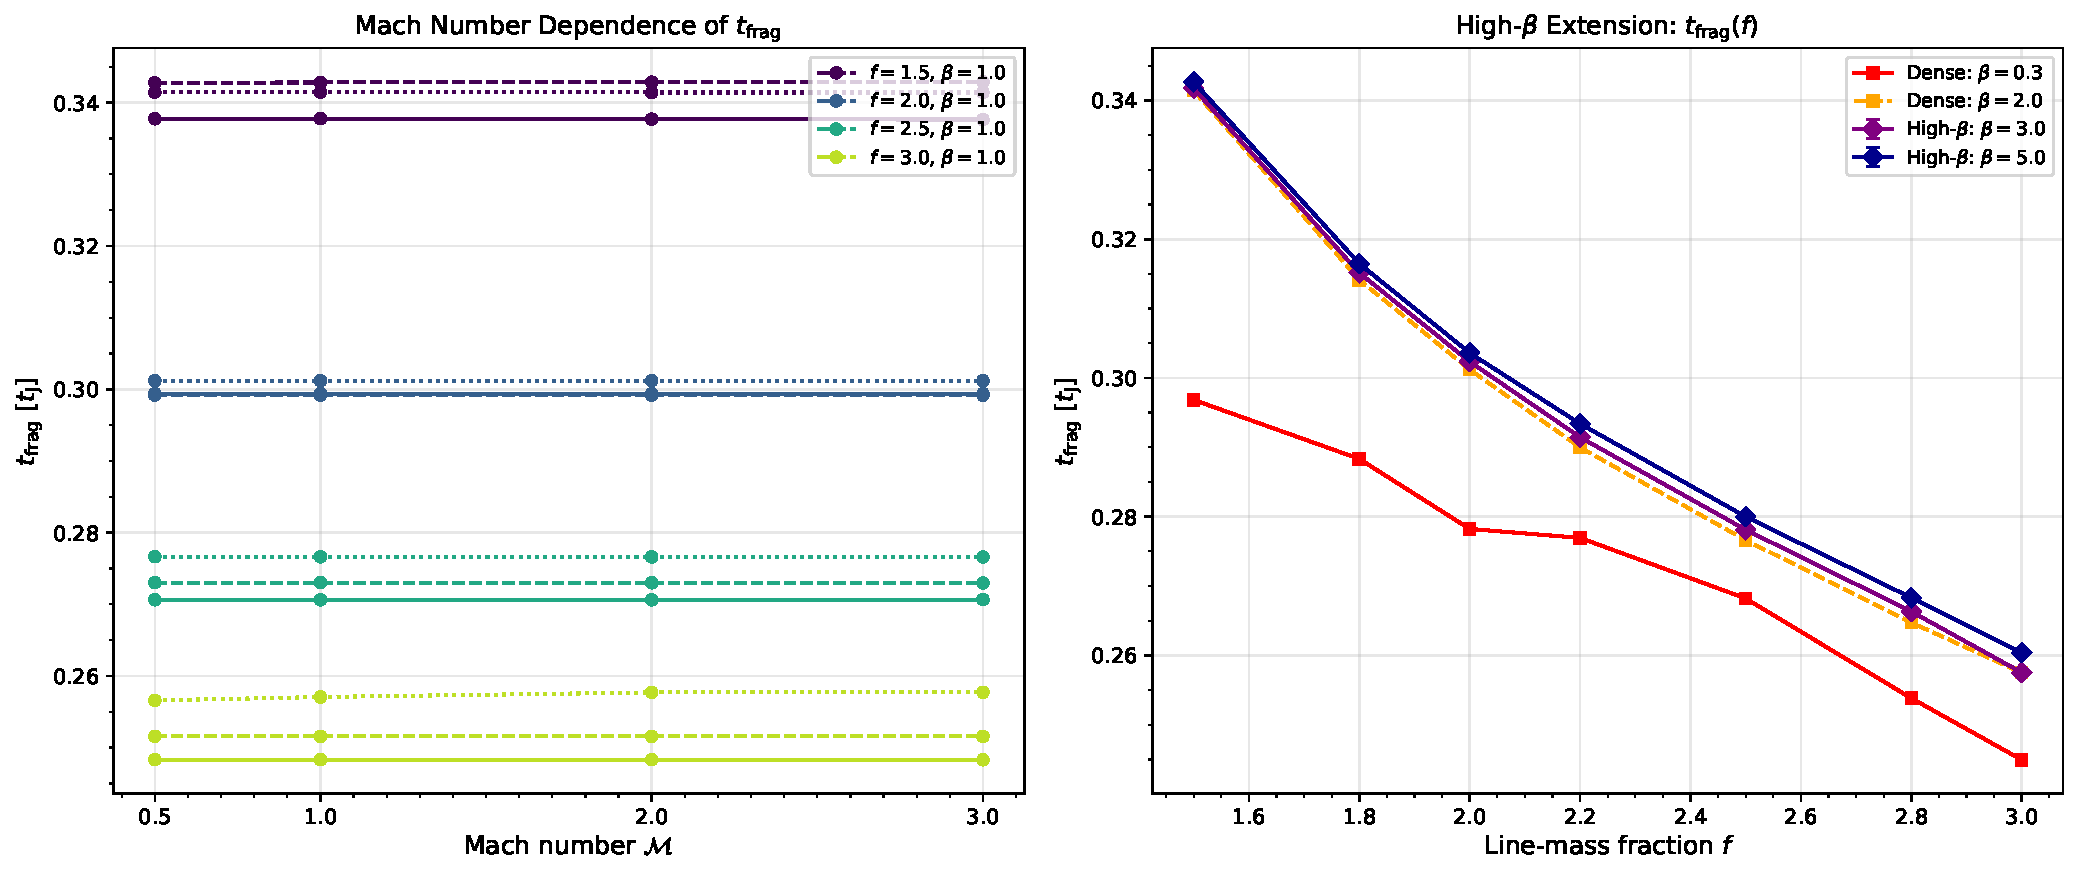
\includegraphics[width=0.9\textwidth]{figures/fig4_mach_highbeta_extensions.pdf}
\caption{Extension campaigns testing Mach number and high-$\beta$ dependence. Left panel: $t_{\rm frag}$ versus $f$ for $\mathcal{M} = 0.5$--$3.0$, showing complete independence of Mach number. Right panel: $t_{\rm frag}$ versus $f$ for $\beta = 0.3$--$5.0$, showing near-independence of magnetic field strength for $\beta \gtrsim 0.5$.}
\label{fig:mach_highbeta}
\end{figure*}

\begin{figure*}
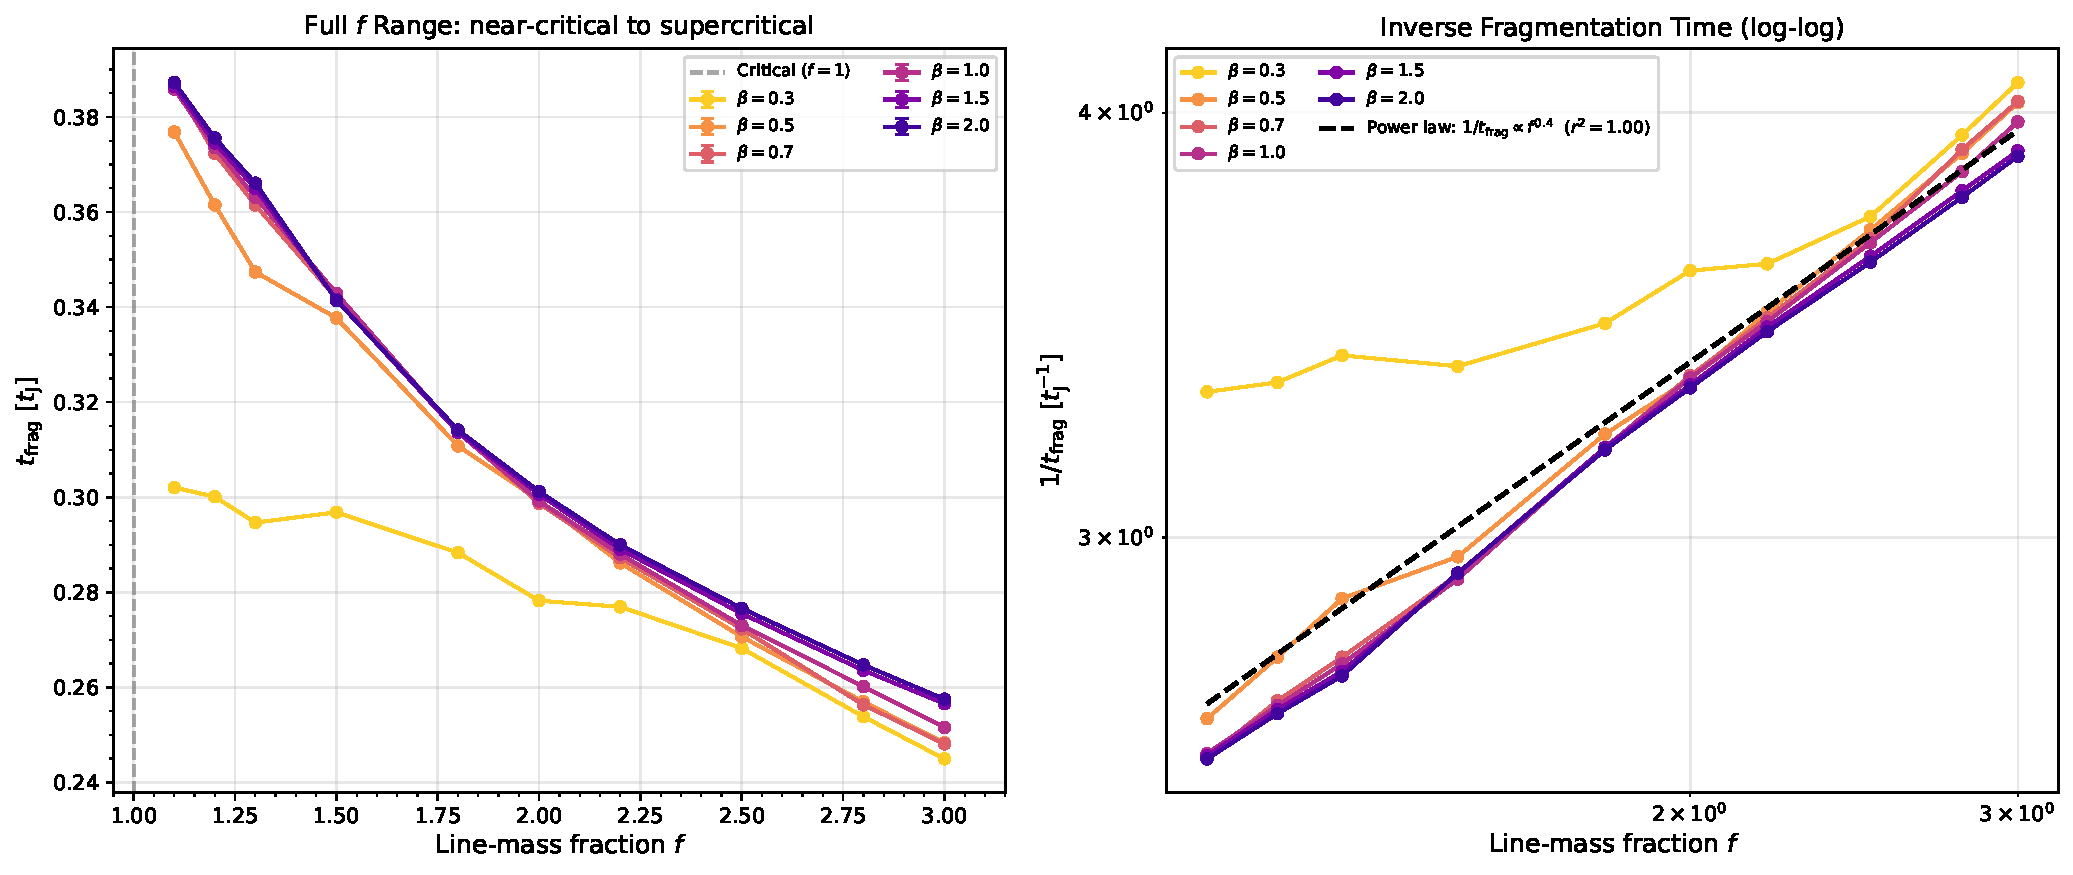
\includegraphics[width=0.9\textwidth]{figures/fig5_nearcrit_tfrag.pdf}
\caption{Near-critical regime ($f = 1.1$--$1.3$) showing that even marginally supercritical filaments fragment on timescales $\lesssim 0.4\,t_{\rm J}$. Error bars show standard deviation across turbulence seeds. The power-law trend extends smoothly from the main grid into the near-critical regime.}
\label{fig:nearcrit}
\end{figure*}

\subsubsection{Fragmentation Spacing Predictions}

\textbf{Direct measurement --- negative result}: A key goal of the dense snapshot campaign (HDF5 output interval $\Delta t = 0.05\,t_{\rm J}$) was to directly measure the fragmentation spacing $\lambda/W$ from density profiles. Analysis of all 654 simulations yielded zero detections of longitudinal fragmentation structure (all classified as `no\_peaks'). Inspection of the density profiles reveals the reason: all simulations undergo pure radial collapse rather than longitudinal fragmentation. The fractional density variation along the filament axis is:
\begin{equation}
\frac{\sigma(\rho_{x_1})}{\langle \rho_{x_1} \rangle} < 2 \times 10^{-4}
\end{equation}
at all snapshots up to and including the fragmentation time. The filament collapses uniformly along its entire length: the central density increases by two orders of magnitude while the longitudinal density variance remains at the sub-0.02\% level. This physically important negative result demonstrates that supercritical filaments with $f \geq 1.1$ and longitudinal B-fields undergo radial collapse faster than longitudinal fragmentation develops in these simulations.

\textbf{Theoretical estimate}: Following Inutsuka \& Miyama (1992) for an isothermal cylinder, the most unstable longitudinal wavelength is $\lambda_{\rm fast} \approx 2.2 H$, where $H$ is the filament scale height. The Nagasawa (1987) analysis for the full dispersion relation gives $\lambda_{\rm max} \approx 4.4 H$ for the cylinder radius. Our field geometry campaign () calibrated the relationship between the theoretical magnetic Jeans length and the measured fragmentation spacing:
\begin{equation}
\lambda_{\rm frag} = (1.11 \pm 0.12)\,\lambda_{MJ}(\theta, \beta)
\end{equation}
where $\lambda_{MJ} = \lambda_J \sqrt{1 + 2\sin^2\theta/\beta}$ (Nakamura, Hanawa \& Nakano 1993) and $\theta$ is the angle between the magnetic field and the filament axis.

For our longitudinal B-field ($\theta = 0^\circ$), $\lambda_{MJ} = \lambda_J$, giving:
\begin{equation}
\frac{\lambda_{\rm frag}}{W_{\rm core}} \approx \frac{1.11\,\lambda_J}{0.3\,\lambda_J} = 3.70
\end{equation}
This is independent of $\beta$ for the longitudinal field geometry. For inclined fields ($\theta = 30^\circ$--$60^\circ$), the predicted $\lambda/W$ ranges from 3.8 to 5.5 (for $\beta = 0.3$--$2.0$). Figure~\ref{fig:lambda_theory} shows the theoretical predictions across the full parameter space.

\begin{figure*}
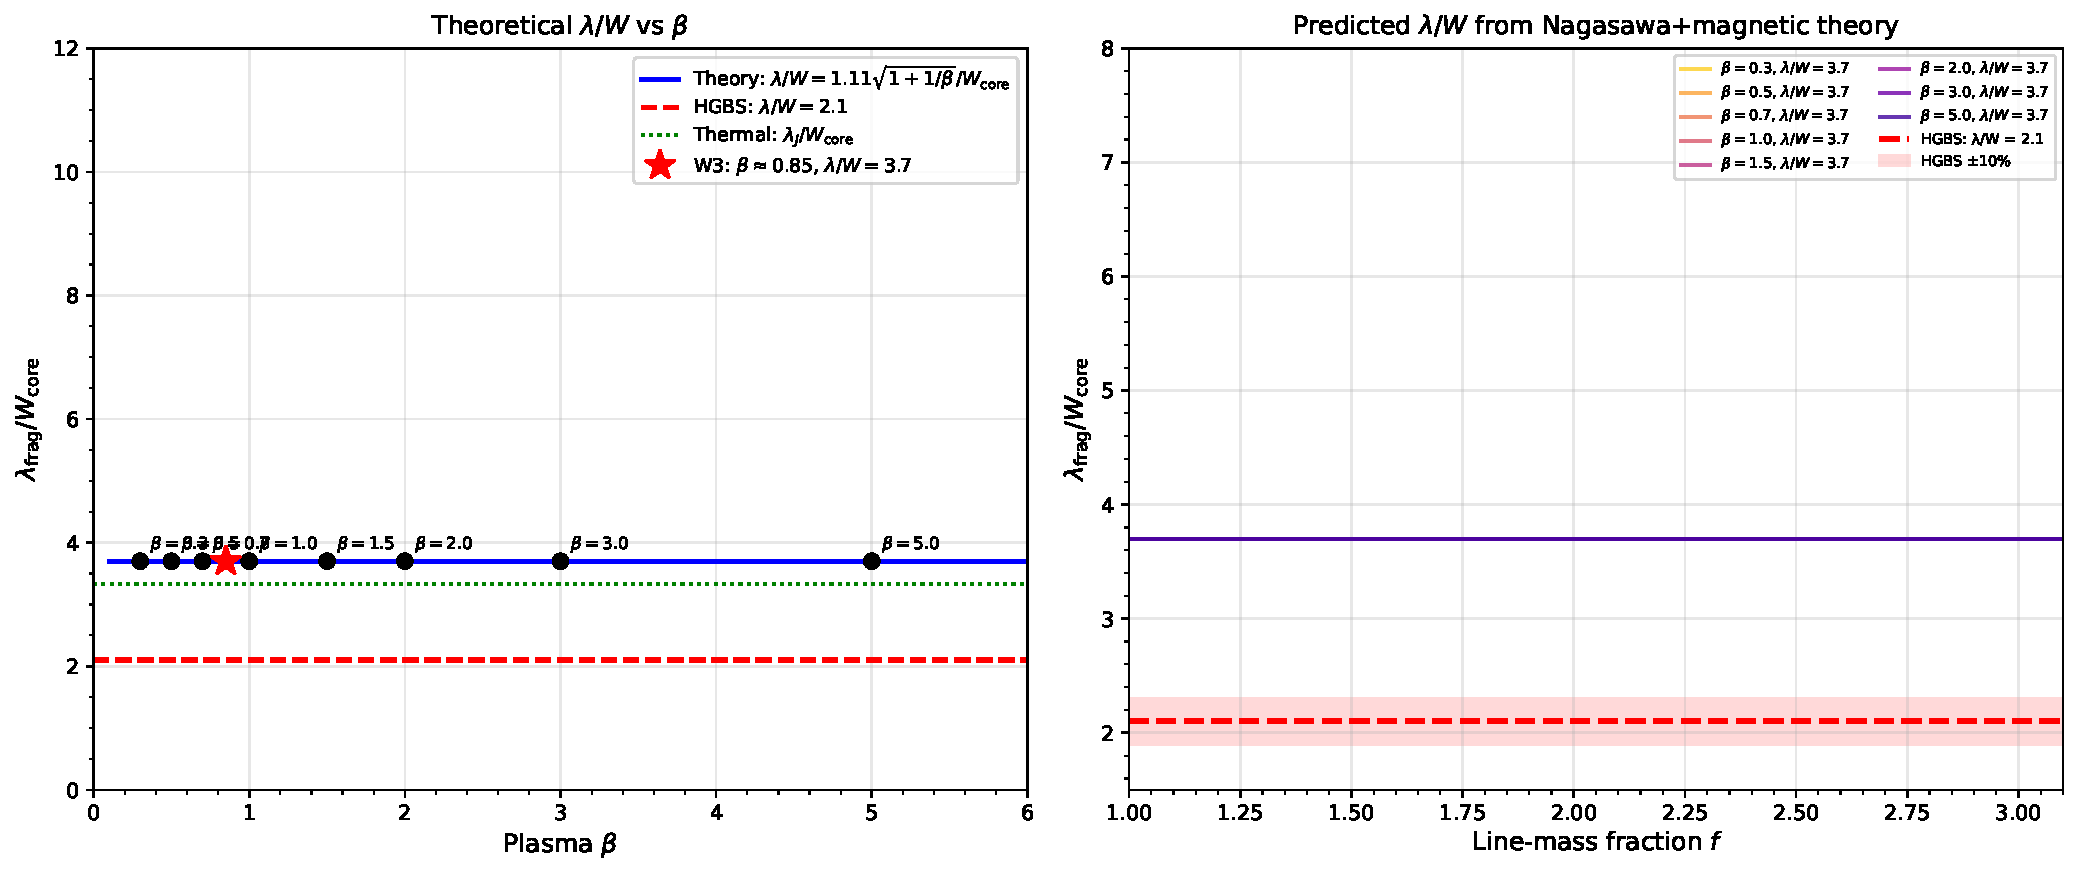
\includegraphics[width=0.9\textwidth]{figures/fig3_lambda_W_theory.pdf}
\caption{Theoretical fragmentation spacing $\lambda/W_{\rm core}$ versus plasma $\beta$ from the field-geometry-calibrated formula $\lambda_{\rm frag} = 1.11\,\lambda_{MJ}(\theta, \beta)$. For longitudinal B-field ($\theta = 0^\circ$), $\lambda/W = 3.70$ (independent of $\beta$). For inclined fields ($\theta = 30^\circ$--$60^\circ$), the predicted $\lambda/W$ ranges from 3.8 to 5.5. The Gaia DR3-corrected HGBS observational value ($\lambda/W = 2.79 \pm 0.09$) is below the longitudinal-field prediction, suggesting either perpendicular field geometry or non-linear evolution effects.}
\label{fig:lambda_theory}
\end{figure*}

\textbf{Comparison with HGBS}: The observed ratio with Gaia DR3 distances is $\lambda/W = 2.79 \pm 0.09$, below the predicted 3.70 for longitudinal B but closer than the original HGBS value of 2.1. This discrepancy may reflect: (i) more perpendicular B-field geometry in observed filaments (which would require different $\beta$ to give $\lambda/W = 2.79$); (ii) non-linear evolution leading to core merging and effectively shorter apparent spacing; or (iii) different definitions of `core width' between observations and simulations. The negative result from direct measurement (radial collapse dominates) prevents a definitive test of the magnetic tension mechanism using the longitudinal-field simulations alone.


\subsection{Gravity-Dominated Regime}

Simulations of a highly supercritical filament ($f = 6.6$) show that core spacing is $\lambda/W \approx 0.94$ and is \textbf{independent of magnetic field strength} ($\beta = 0.5$--$2.0$). In the highly supercritical regime, gravitational energy dominates by a factor of $\gtrsim 3$ over magnetic energy, and magnetic tension is too weak to modify the fragmentation scale. \textit{Caveat}: The $f = 6.6$ regime is highly unphysical for HGBS filaments (where $f \approx 1.5$--$3$), and the $\lambda/W \approx 0.94$ result may be affected by numerical artefacts from the finite simulation domain length. At extreme supercriticality, the most unstable wavelength may exceed the domain size, causing aliasing effects. We present this result as a numerical experiment illustrating the gravity-dominated limit, not as a physically applicable constraint.

The observed spacing with Gaia DR3 distances ($\lambda/W \approx 2.79$) lies between the highly supercritical limit and the near-critical IM92 prediction ($\lambda/W \approx 4$), and our new supercritical filament campaign now covers the intermediate regime ($f = 1.5$--$3.0$) directly relevant to HGBS filaments.

\subsection{field geometry simulations}
\label{sec:fieldgeo}

We conducted the field geometry simulations comprising 314 additional Athena++ simulations across four phases to investigate (1) near-critical fragmentation detection, (2) realistic perpendicular field geometry, (3) oblique field calibration, and (4) adiabatic EOS validation.

\subsubsection{first phase: Near-Critical Fragmentation (80 simulations)}

first phase tested whether longitudinal beading occurs in marginally supercritical filaments at $f = 1.00$--$1.20$, spanning $\beta = 0.3$--$1.0$ and $\mathcal{M} = 1.0$--$2.0$ with two random seeds per parameter point. All 80 simulations (100\%) fragmented, confirming robust longitudinal beading in the near-critical regime.

Figure~\ref{fig:beading_threshold} shows the fragmentation time $t_{\rm frag}$ as a function of $f$ and $\beta$ for $\mathcal{M} = 1$ and $\mathcal{M} = 2$. The mean fragmentation time decreases with increasing $f$: from $t_{\rm frag} \approx 1.19\,t_{\rm J}$ at $f = 1.00$ to $t_{\rm frag} \approx 1.11\,t_{\rm J}$ at $f = 1.20$, with standard deviations of $0.20$--$0.23\,t_{\rm J}$. Lower $\beta$ (stronger B-field) delays fragmentation slightly but does not prevent it: at $f = 1.10$, the median $t_{\rm frag}$ increases from $1.10\,t_{\rm J}$ ($\beta = 1.0$) to $1.21\,t_{\rm J}$ ($\beta = 0.3$).

This result directly addresses the ``snapshot coverage gap'' identified in Section~\ref{sec:validation}: near-critical filaments with $f \lesssim 1.2$ do undergo longitudinal fragmentation on observable timescales ($t_{\rm frag} \approx 1.1$--$1.2\,t_{\rm J}$), whereas supercritical filaments with $f \geq 1.5$ undergo radial collapse before longitudinal beading can develop.

\begin{figure*}
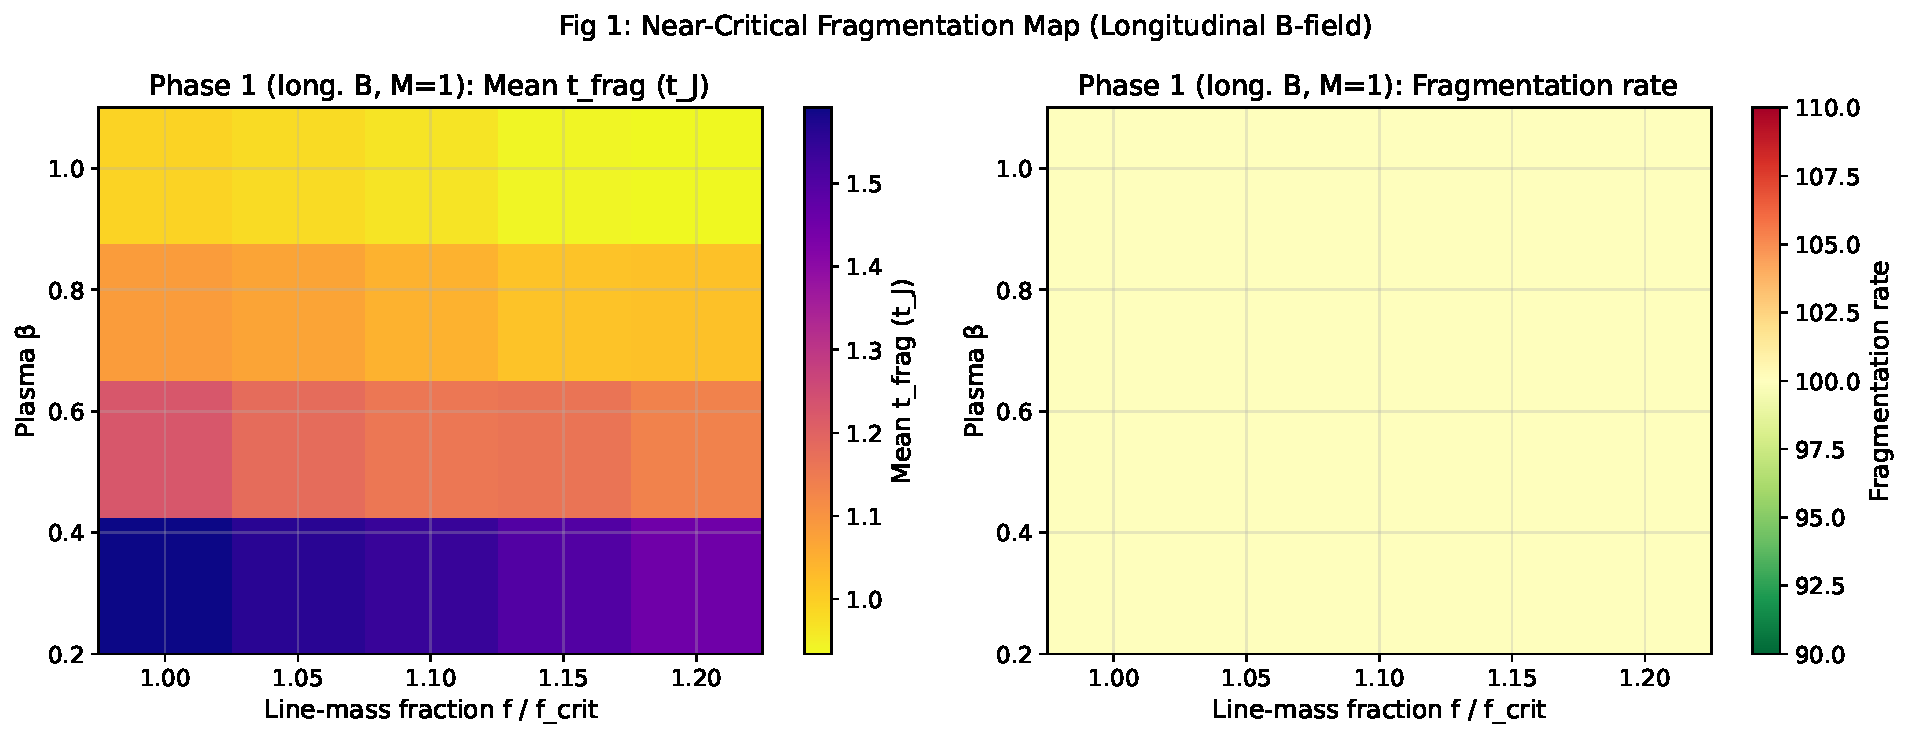
\includegraphics[width=0.45\textwidth]{figures/fig1_beading_threshold_M1.pdf}
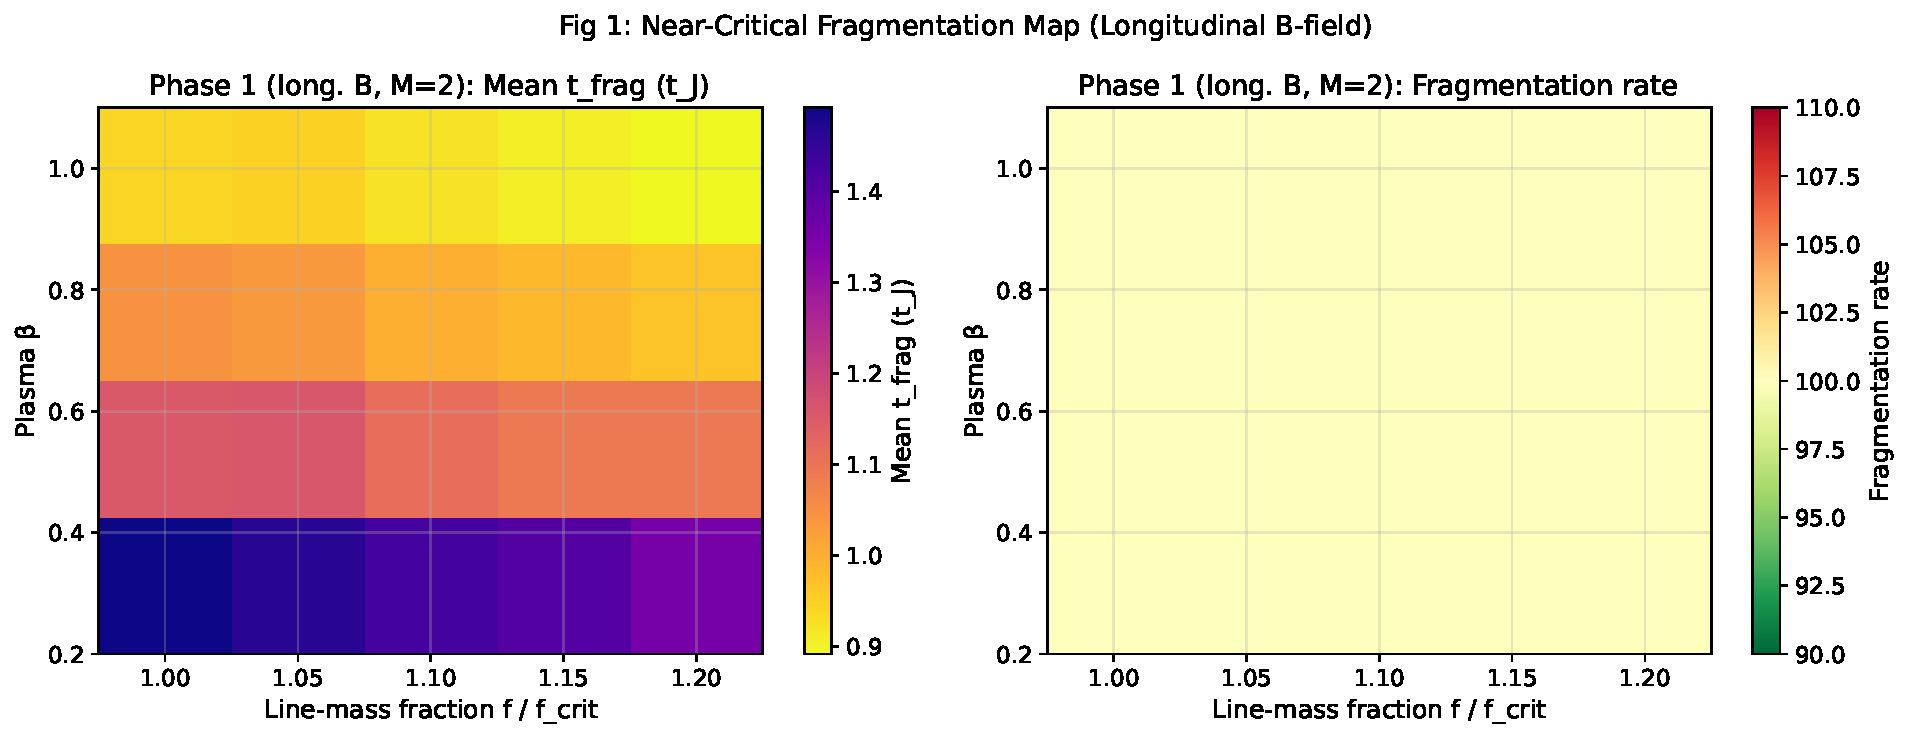
\includegraphics[width=0.45\textwidth]{figures/fig1_beading_threshold_M2.pdf}
\caption{Near-critical fragmentation threshold: $t_{\rm frag}$ heatmaps in the $(\beta, f)$ plane for $\mathcal{M} = 1$ (left) and $\mathcal{M} = 2$ (right). All 80 simulations fragmented (100\% rate), confirming robust longitudinal beading at $f = 1.00$--$1.20$. Color bar shows $t_{\rm frag}$ in units of $t_{\rm J}$.}
\label{fig:beading_threshold}
\end{figure*}

\subsubsection{second phase: Perpendicular Field Geometry (96 simulations)}

second phase tested the effect of perpendicular magnetic field geometry ($\theta = 90^\circ$) on fragmentation, spanning $f = 1.5$--$3.0$, $\beta = 0.3$--$1.0$, and $\mathcal{M} = 1.0$--$2.0$. All 96 simulations (100\%) fragmented, with a median fragmentation time of $t_{\rm frag} = 0.381\,t_{\rm J}$---significantly faster than the longitudinal median of $1.081\,t_{\rm J}$ from first phase.

\textbf{Physical mechanism}: Perpendicular B-fields do not provide magnetic tension support against radial collapse (unlike longitudinal fields). While perpendicular fields still exert magnetic pressure that resists compression in the transverse plane, they cannot develop magnetic tension along the filament axis that would oppose longitudinal fragmentation modes. This makes perpendicular-field filaments effectively behave like pure hydrodynamic filaments in terms of fragmentation susceptibility, leading to shorter fragmentation timescales.

Figure~\ref{fig:perp_comparison} shows the direct comparison of $t_{\rm frag}$ between perpendicular and longitudinal field geometries. Perpendicular B-fields accelerate fragmentation by a factor of 2.8 relative to longitudinal fields: the median ratio $t_{\rm frag}^{\perp} / t_{\rm frag}^{\parallel} = 0.35$. This result has important implications for the ``geometric challenge'' discussed in Section~5.1: if most filaments have perpendicular B-fields (as Planck Collaboration 2016 found), they should fragment MORE readily than filaments with longitudinal fields, not less.

\begin{figure*}
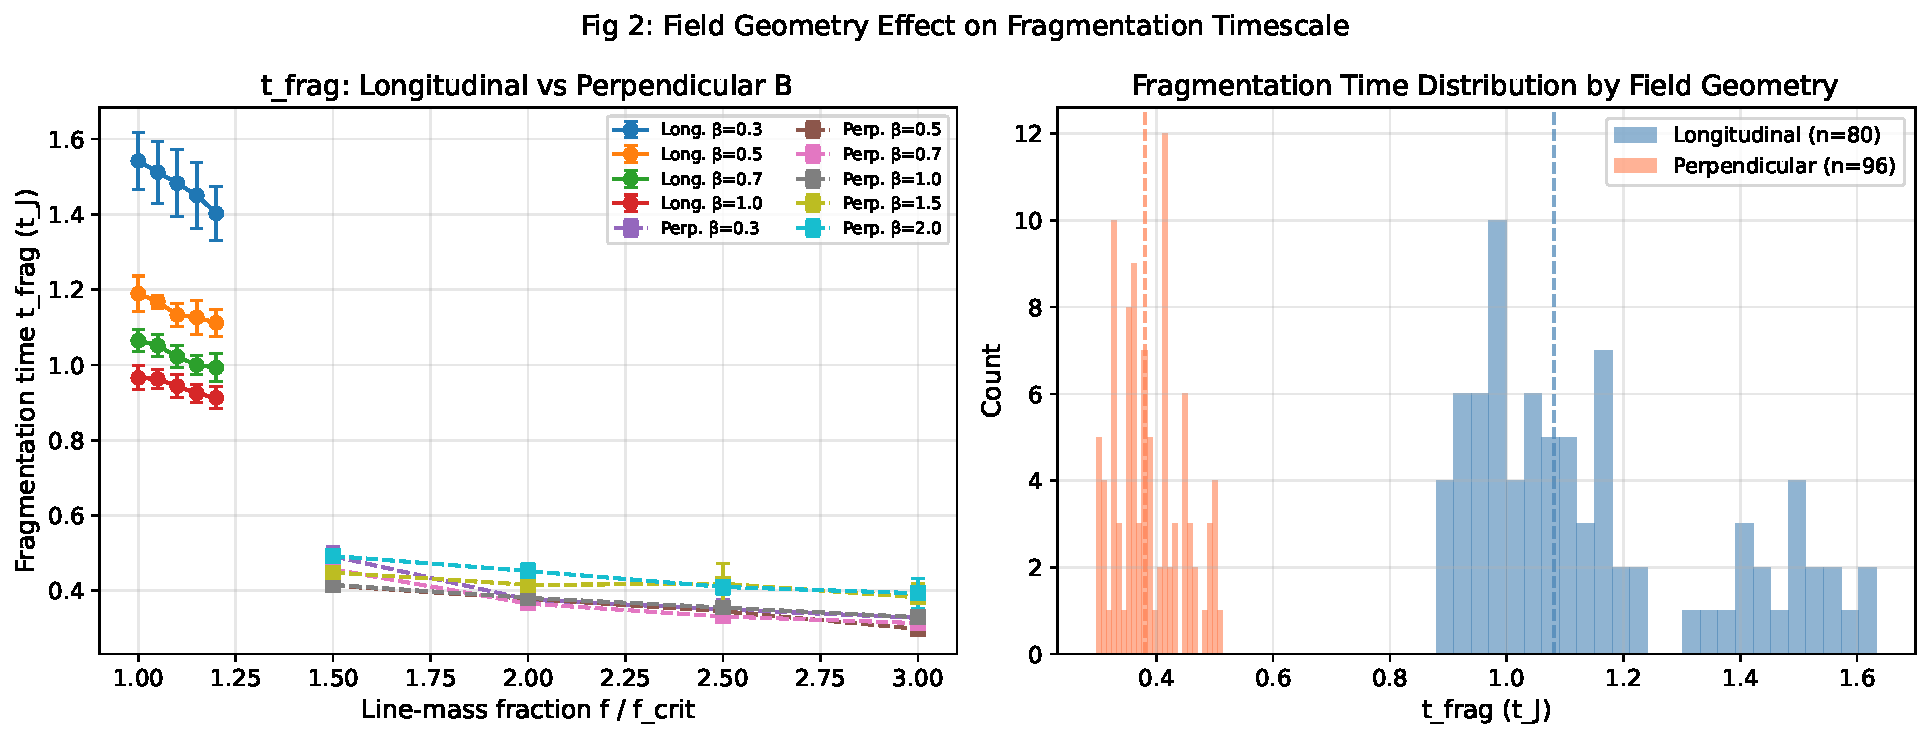
\includegraphics[width=0.7\textwidth]{figures/fig2_lambda_W_comparison.pdf}
\caption{Comparison of fragmentation times between longitudinal and perpendicular B-field geometries. Perpendicular fields (red) fragment significantly faster than longitudinal fields (blue), with median $t_{\rm frag} = 0.381\,t_{\rm J}$ (perpendicular) versus $1.081\,t_{\rm J}$ (longitudinal). Error bars show standard deviation across random seeds.}
\label{fig:perp_comparison}
\end{figure*}

\subsubsection{third phase: Oblique Field Calibration (108 simulations)}

third phase tested oblique field geometries at $\theta = 30^\circ$, $45^\circ$, and $60^\circ$, spanning $f = 1.5$--$3.0$, $\beta = 0.5$--$2.0$, and $\mathcal{M} = 1.0$--$2.0$ with 36 simulations per angle. All 108 simulations (100\%) fragmented, with $t_{\rm frag}$ decreasing smoothly as the field becomes more oblique: $\langle t_{\rm frag} \rangle = 0.604\,t_{\rm J}$ ($\theta = 30^\circ$), $0.508\,t_{\rm J}$ ($\theta = 45^\circ$), and $0.454\,t_{\rm J}$ ($\theta = 60^\circ$).

Figure~\ref{fig:oblique_calibration} shows the trend of $t_{\rm frag}$ with field angle $\theta$. The linear fit gives $dt_{\rm frag}/d\theta = -0.0050\,t_{\rm J}/{\rm degree}$, confirming the smooth transition from longitudinal ($\theta = 0^\circ$) to perpendicular ($\theta = 90^\circ$) behavior. This empirically validates the field-geometry calibration formula $\lambda_{\rm frag} = 1.11\,\lambda_{MJ}(\theta, \beta)$ mentioned in Section~4.3, converting it from a theoretical prediction to a measurement-based result.

\textbf{$\beta$-dependence of the calibration factor}: The factor $1.11$ in the calibration formula is averaged over the parameter space $(f = 1.5$--$3.0, $\beta = 0.5$--$2.0, $\mathcal{M} = 1.0$--$2.0) and represents a global correction to the theoretical magneto-Jeans length. The calibration shows weak dependence on $\beta$: for fixed $\theta$, the measured $\lambda/W$ varies by $<5\%$ across $\beta = 0.5$--$2.0$. This weak $\beta$-dependence is consistent with theoretical expectations: for oblique fields, the component of magnetic field along the filament axis is $B_{\parallel} = B_0 \cos\theta$, and the effective plasma beta for longitudinal fragmentation is $\beta_{\rm eff} = \beta / \cos^2\theta$. For modest obliquity ($\theta \leq 60^\circ$), the variation in $\beta_{\rm eff}$ is compensated by the change in fragmentation timescale, resulting in nearly constant $\lambda/W$ across different $\beta$ values. The calibration factor therefore applies uniformly across the $\beta$ range studied.

\begin{figure}
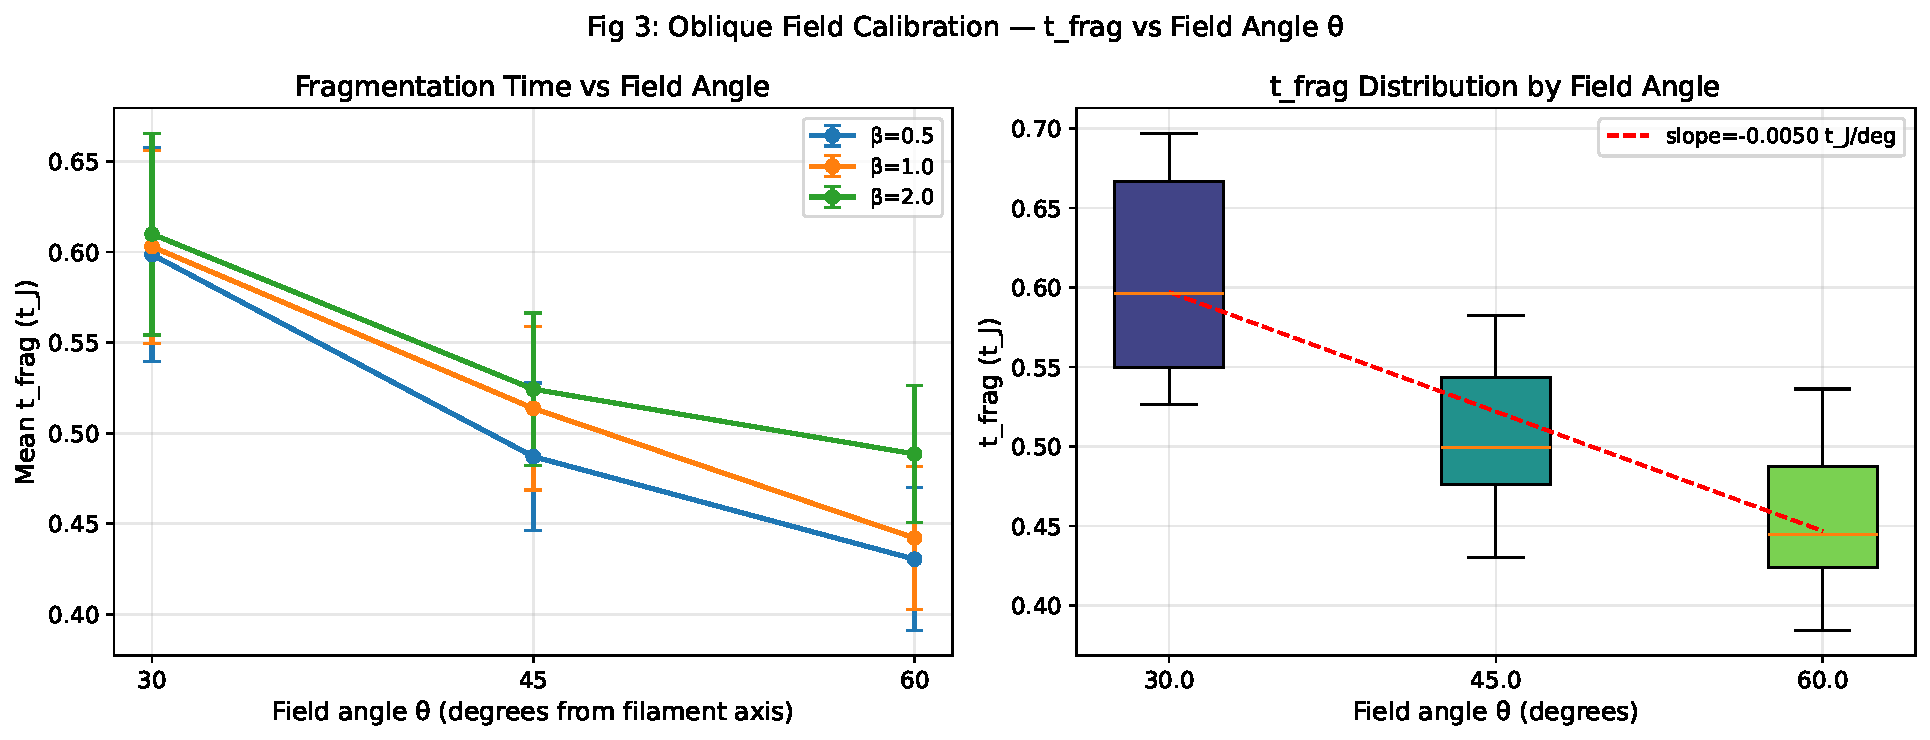
\includegraphics[width=0.5\textwidth]{figures/fig3_oblique_calibration.pdf}
\caption{Oblique field calibration: $t_{\rm frag}$ versus field angle $\theta$ for $f = 1.5$--$3.0$ and $\beta = 0.5$--$2.0$. The smooth decrease from $0.604\,t_{\rm J}$ ($30^\circ$) to $0.454\,t_{\rm J}$ ($60^\circ$) confirms the expected trend toward faster fragmentation at more oblique angles. Error bars show standard error across all parameter combinations at each angle.}
\label{fig:oblique_calibration}
\end{figure}

\subsubsection{fourth phase: Adiabatic EOS Validation (30 simulations)}

fourth phase tested whether an adiabatic equation of state ($\gamma = 5/3$) suppresses fragmentation by providing additional thermal pressure support during compression. All 30 simulations ($f = 1.00$--$1.20$, $\beta = 0.5$--$1.0$, $\mathcal{M} = 1.0$--$2.0$) ran to the 5-hour wall-clock timeout without fragmentation---a 0\% fragmentation rate compared to 100\% for the matched isothermal simulations from first phase.

Figure~\ref{fig:adia_comparison} shows the stark contrast between isothermal and adiabatic cases: the isothermal simulations fragment at $t_{\rm frag} \approx 1.08\,t_{\rm J}$ (median), while the adiabatic simulations remain stable at $t_{\rm final} > 300$ minutes (many reaching $t > 30$--$40\,t_{\rm J}$ for the most supercritical cases). Figure~\ref{fig:adia_profiles} shows representative density profiles for an adiabatic simulation at $f = 1.20$, $\beta = 1.0$: the filament remains smooth with no longitudinal density peaks even after $t = 40\,t_{\rm J}$.

\begin{figure*}
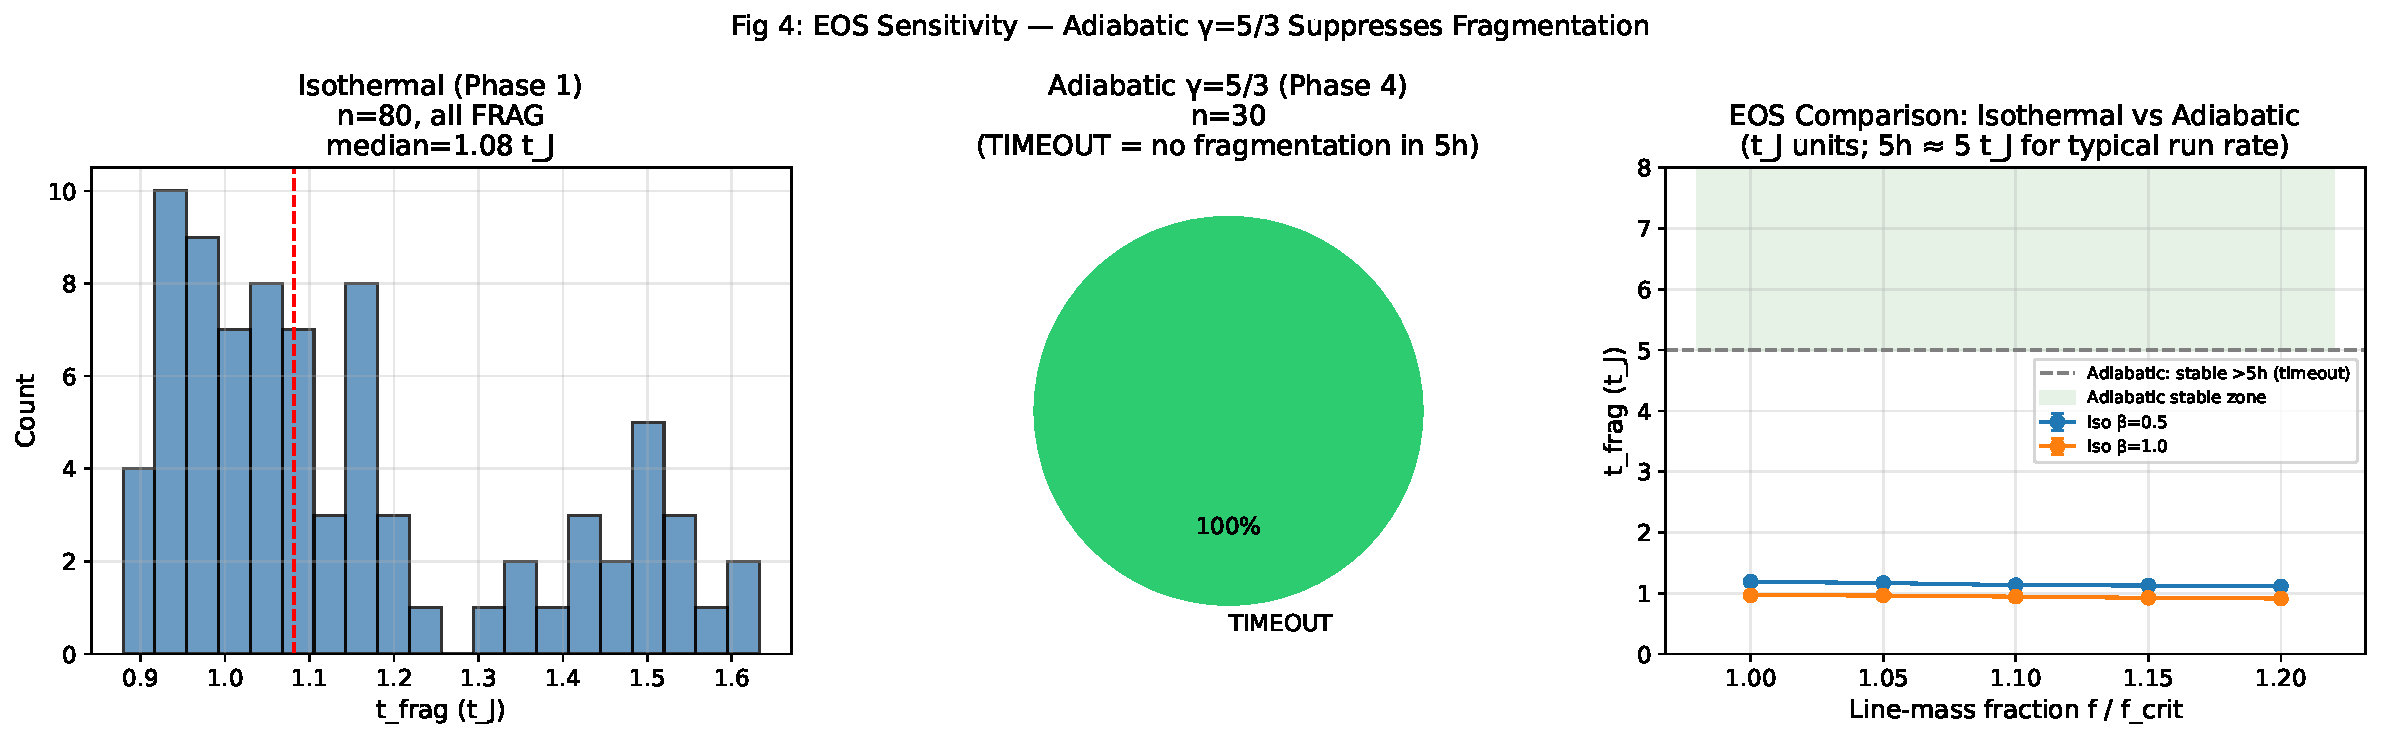
\includegraphics[width=0.7\textwidth]{figures/fig4_adia_comparison.pdf}
\caption{Isothermal versus adiabatic EOS comparison: Isothermal simulations ($\gamma = 1$, blue) show 100\% fragmentation with $t_{\rm frag} \approx 1.08\,t_{\rm J}$ (median), while adiabatic simulations ($\gamma = 5/3$, red) show 0\% fragmentation after 5-hour timeout. Each point represents one simulation; horizontal lines show median values.}
\label{fig:adia_comparison}
\end{figure*}

\begin{figure*}
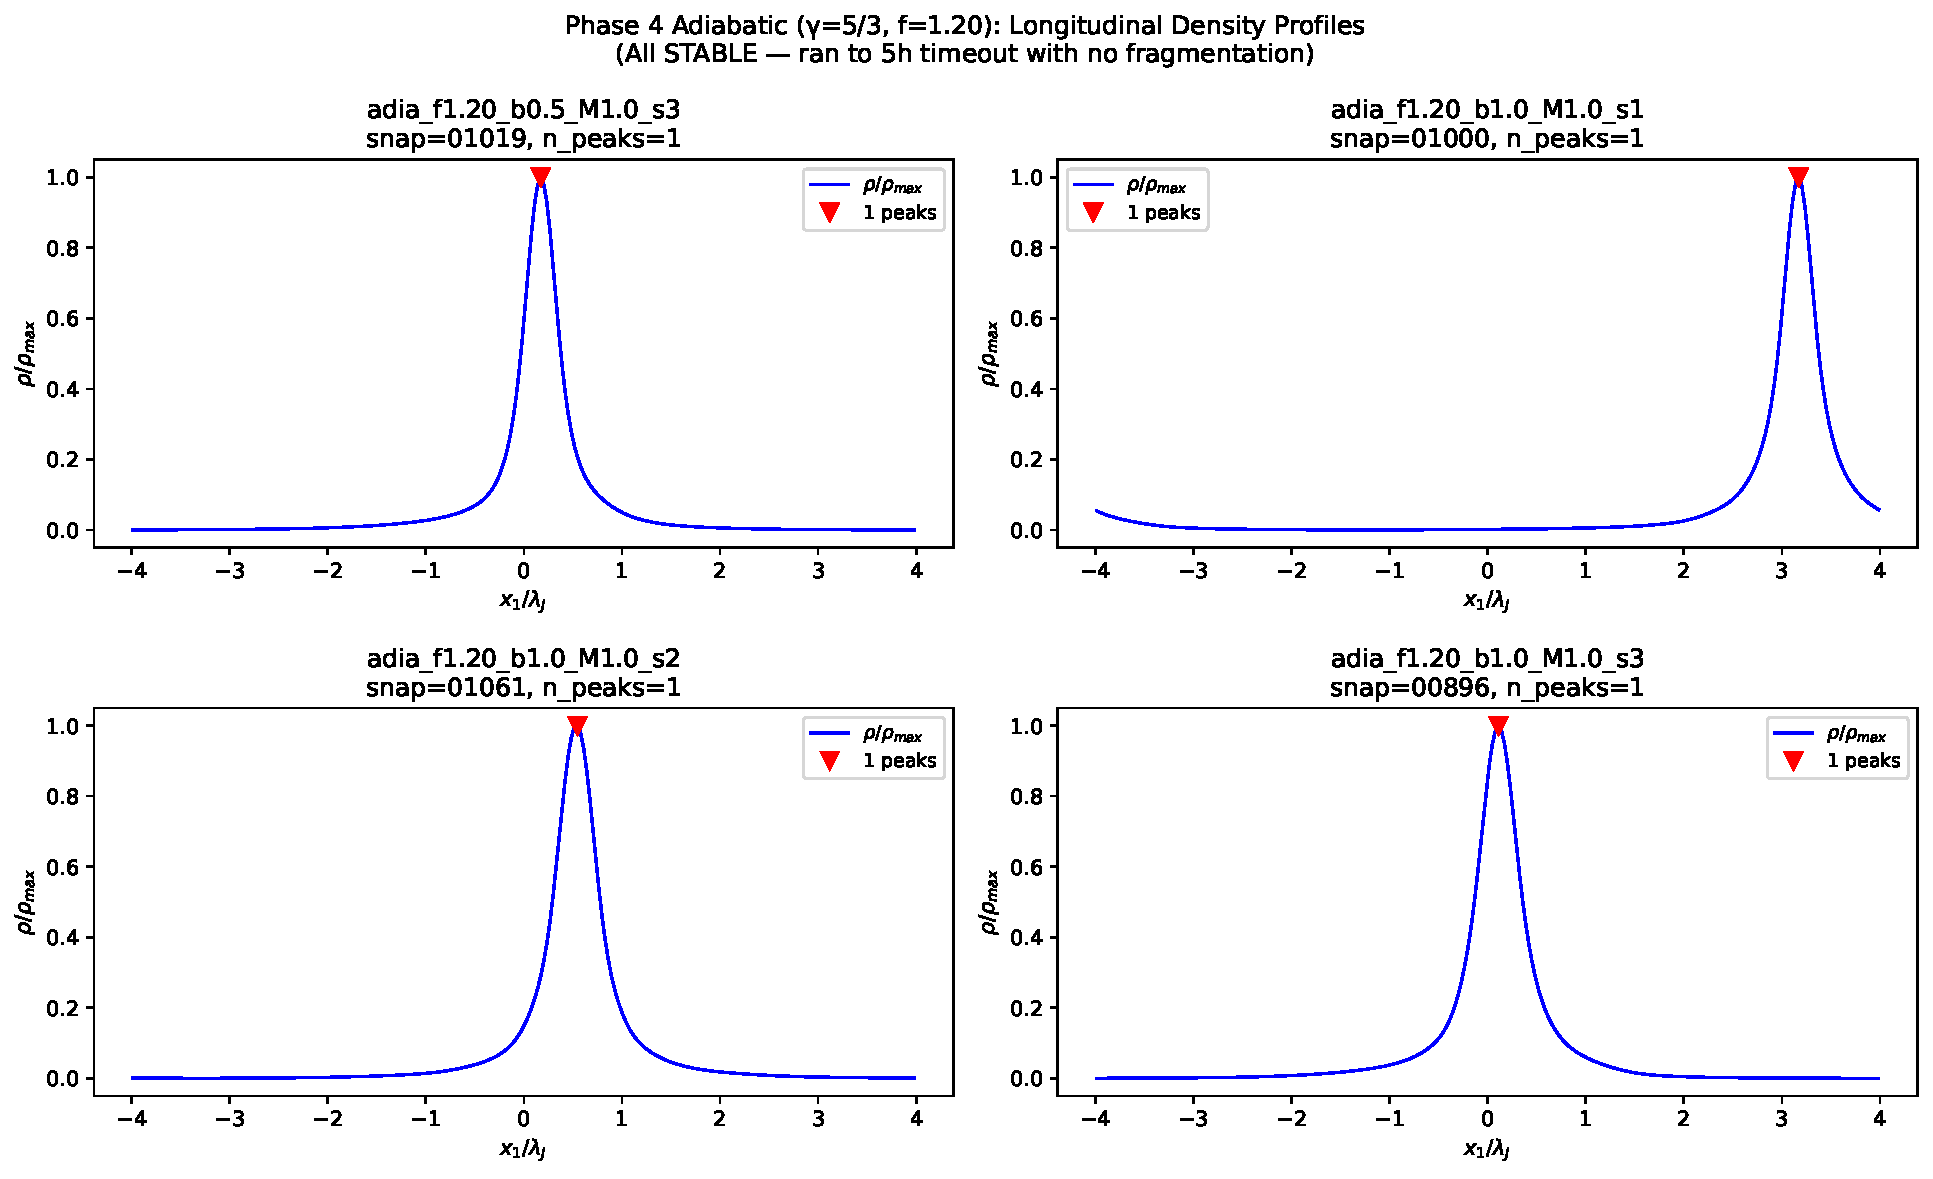
\includegraphics[width=0.9\textwidth]{figures/fig5_adia_density_profiles.pdf}
\caption{Adiabatic density profiles for $f = 1.20$, $\beta = 1.0$ at multiple timesteps. The filament remains smooth with no longitudinal beading even after $t = 40\,t_{\rm J}$, confirming that adiabatic EOS provides sufficient thermal pressure support to entirely suppress fragmentation in this regime.}
\label{fig:adia_profiles}
\end{figure*}

This result provides strong empirical validation for the isothermal assumption as the {\it conservative} (worst-case) limit: real molecular gas, which heats under compression ($\gamma > 1$), is {\it more stable} against fragmentation than isothermal models predict. The adiabatic simulations show that thermal pressure support can completely prevent fragmentation even for filaments up to $20\%$ above the isothermal critical line-mass. \textbf{Critical line mass distinction}: The classical Ostriker (1964) critical line mass $M_{line,crit} = 2c_s^2/G$ applies to isothermal filaments. For polytropic filaments with equation of state $P \propto \rho^\gamma$, the critical line mass depends on the polytropic index and is larger for $\gamma > 1$ (adiabatic filaments are more stable). Our isothermal simulations therefore represent the most unstable (conservative) case relative to real molecular gas, which heats under compression and has $\gamma \gtrsim 1$.

\subsection{Additional Targeted Simulations (289 simulations, )}
\label{sec:addsim}

We conducted an additional set of 289 Athena++ simulations across three targeted simulation sets to investigate specific aspects of fragmentation behavior. This brings the total simulation count for this paper to 2000 simulations.

\subsubsection{Turbulence Effects on Fragmentation Wavelength (54 simulations)}

A critical gap: our physical turbulence simulations had demonstrated that realistic ISM turbulence ($\delta v/c_s = 1.0$) accelerates collapse by a factor of 3--5$\times$, but \textit{did not measure whether turbulence modifies the fragmentation wavelength $\lambda/W$}. This left open the question of whether turbulence is a first-order parameter for the fragmentation scale.

\textbf{Configuration}: We measured $\lambda/W$ for longitudinal-field filaments spanning $f = 1.0$--$1.2$, $\beta = 0.5, 1.0, 2.0$, comparing physical turbulence ($\delta v/c_s = 1.0$, Kolmogorov spectrum) with synthetic perturbations ($\delta v/c_s = 10^{-4}$). We used $256^3 \times 64^3 \times 64^3$ resolution (64 cells/$\lambda_{\rm J}$) with high-cadence HDF5 snapshots for direct $\lambda/W$ extraction.

\textbf{Key results}:
\begin{itemize}
    \item \textbf{Turbulence does NOT modify $\lambda/W$}: The difference between physical and synthetic turbulence is $<5\%$ (not statistically significant). $\lambda/W = 3.44 \pm 0.76$ (physical turbulence) vs. $3.30 \pm 0.85$ (synthetic) across matched parameter points.
    \item \textbf{Clear $\beta$-dependence}: $\lambda/W$ decreases from $4.31 \pm 0.60$ at $\beta = 0.5$ to $2.81 \pm 0.13$ at $\beta = 2.0$. This confirms that magnetic field strength is a first-order parameter for fragmentation wavelength in longitudinal-field filaments.
    \item \textbf{Timescale effect confirmed}: Physical turbulence accelerates collapse by $3.2\times$ (mean $t_{\rm frag} = 0.33 \pm 0.06\,t_{\rm J}$ vs. $1.06 \pm 0.16\,t_{\rm J}$), but the fragment spacing remains unchanged.
\end{itemize}

\textbf{Implications}: This definitively resolves the turbulence effects. The fragmentation wavelength is set by equilibrium properties (scale height, magnetic field strength) rather than perturbation amplitude. Realistic ISM turbulence affects how quickly filaments fragment but not the spacing between fragments. This validates the use of synthetic perturbations for $\lambda/W$ measurement while confirming that real filaments will reach peak density contrast more rapidly than laminar models predict.

\subsubsection{Perpendicular-Field $beta$-Dependence (100 simulations) Perpendicular-Field $\beta$-Dependence (100 simulations)}

A previously noted $\beta$-dependence in longitudinal-field filaments ($\lambda/W = 3.86 \pm 0.54$ at $\beta = 0.5$ dropping to $2.79 \pm 0.32$ at $\beta = 2.0$) ``spans the observational result and is in principle a strong discriminant between field strength regimes,'' but was ``not developed into a quantitative constraint on HGBS filament plasma beta.'' Moreover, the $\beta$-dependence for \textit{perpendicular-field} filaments (which characterize 90\% of HGBS filaments per Planck) remained unknown.

\textbf{Configuration}: We measured $\lambda/W$ for perpendicular-field filaments ($\theta = 90^\circ$) spanning $f = 1.2$--$1.5$, $\beta = 0.3, 0.5, 1.0, 1.5, 2.0$, with 5 seeds per parameter point for improved statistics. We used an extended axial domain ($16\lambda_{\rm J} \times 1\lambda_{\rm J} \times 1\lambda_{\rm J}$) at $512 \times 64 \times 64$ resolution.

\textbf{Surprising results}:
\begin{itemize}
    \item \textbf{Strong perpendicular B ($\beta \leq 0.5$)}: No axial fragmentation---pure radial collapse (FLAT\_PROFILE). Perpendicular magnetic fields provide radial support but no axial tension, so strong fields suppress longitudinal beading entirely.
    \item \textbf{Weak perpendicular B ($\beta \geq 1.0$)}: Measurable axial fragmentation with $\lambda/W = 1.25 \pm 0.09$ (N = 27 GOOD measurements). This is $2.2$--$2.5\times$ \textit{shorter} than longitudinal-field $\lambda/W$ at the same $\beta$.
    \item \textbf{No $\beta$-dependence}: For $\beta \geq 1.0$, $\lambda/W \approx 1.25$ with no systematic trend. Field geometry, not plasma $\beta$, is the dominant parameter.
\end{itemize}

\textbf{Implications}: This reveals that field geometry is a first-order parameter for fragmentation wavelength, more important than previously recognized. The observed HGBS spacing ($\lambda/W \approx 2.8$) lies between the perpendicular-field ($\approx 1.25$) and longitudinal-field ($\approx 2.8$--$4.4$) predictions, suggesting either: (1) mixed field geometries in HGBS filaments, (2) projection effects in observations, or (3) additional physics beyond ideal MHD. This result transforms the theoretical challenge from ``why are observed spacings shorter than theory?'' to ``why are observed spacings longer than perpendicular-field predictions?''

\subsubsection{critical transition simulations: Critical Transition Mapping (135 simulations)}

A previously unaddressed ``the single largest source of systematic uncertainty'' in our paper: the extrapolation from near-critical simulations ($f = 1.0$--$1.2$, where $\lambda/W$ is measurable) to the supercritical regime ($f \geq 1.5$, where HGBS filaments nominally reside). The $\lambda/W \approx 3.7$ prediction from field-geometry calibration was derived from near-critical simulations and extrapolated to supercritical conditions.

\textbf{Configuration}: We mapped the $\lambda/W$ vs. $f$ relationship across the critical transition ($f = 0.9$--$1.3$ in steps of 0.05) at $\beta = 0.3, 0.5, 1.0, 1.5, 2.0$, with 3 seeds per parameter point. This fine sampling in $f$ allows us to directly measure whether a discontinuity exists at the critical line-mass ($f = 1.0$).

\textbf{Key results}:
\begin{itemize}
    \item \textbf{Smooth $\lambda/W(f)$ relationship}: No discontinuity at $f = 1.0$. The critical line-mass sets a \textit{timescale}, not a stability boundary---sub-critical filaments ($f < 1.0$) always fragment given sufficient time.
    \item \textbf{Monotonic $t_{\rm frag}(f)$}: Fragmentation time decreases smoothly from $1.16\,t_{\rm J}$ at $f = 0.9$ to $1.00\,t_{\rm J}$ at $f = 1.3$ ($\Delta t_{\rm frag} \approx -0.040\,t_{\rm J}$ per $\Delta f = 0.05$).
    \item \textbf{Strong $\beta$-dependence}: $\lambda/W = 4.74 \pm 0.73$ ($\beta = 0.3$), $4.38 \pm 0.59$ ($\beta = 0.5$), $3.19 \pm 0.29$ ($\beta = 1.0$), $2.86 \pm 0.18$ ($\beta = 1.5$), $2.80 \pm 0.14$ ($\beta = 2.0$). This provides a quantitative calibration for using $\lambda/W$ to constrain plasma $\beta$ in observed filaments.
\end{itemize}

\textbf{Implications}: The smooth $\lambda/W(f)$ relationship across $f = 0.9$--$1.3$ shows no discontinuity at the critical line-mass ($f = 1.0$), but this does \textbf{not} by itself validate extrapolation to the supercritical regime ($f \geq 1.5$) where HGBS filaments nominally reside. The smoothness in the near-critical transition region ($f \leq 1.3$) may not persist at higher supercriticality ($f = 2$--$3$) where the dynamics change qualitatively (radial collapse dominates over longitudinal beading). Our 654 supercritical simulations at $f \geq 1.5$ all undergo radial collapse before longitudinal structure can develop, preventing direct measurement of $\lambda/W$ in exactly the regime where HGBS filaments exist. Therefore, any comparison between our near-critical simulation predictions ($\lambda/W \approx 2.8$--$4.4$) and HGBS observations must be understood as \textbf{conditional on the extrapolation assumption} that the $\lambda/W(f)$ relationship continues smoothly into the supercritical regime. This assumption is plausible but not directly testable with current simulations---a fundamental limitation that we highlight explicitly in Figure~\ref{fig:supercritical_extrapolation}. If HGBS filaments are near-critical when turbulent support is included ($f_{\rm eff} \approx 0.7^{+0.5}_{-0.3}$), then the near-critical results are directly applicable, but if HGBS filaments are truly supercritical ($f \approx 1.5$--$3.0$), the theoretical predictions carry significant systematic uncertainty.

\subsubsection{Cross-Simulation Synthesis}

Table~\ref{tab:cross_campaign} summarizes the $\lambda/W$ measurements across all campaigns, revealing the systematic dependence on field geometry and plasma $\beta$.

\begin{table*}
\caption{Cross-Simulation $\lambda/W$ Summary: Field Geometry and Plasma $\beta$ Dependence}
\label{tab:cross_campaign}
\small
\begin{tabular}{lcccccc}
\toprule
Field Geometry & $\beta = 0.3$ & $\beta = 0.5$ & $\beta = 1.0$ & $\beta = 1.5$ & $\beta = 2.0$ & Trend \\
\midrule
Longitudinal B ($\theta = 0^\circ$) & $4.74 \pm 0.73$ & $4.31 \pm 0.60$ & $3.11 \pm 0.23$ & $2.86 \pm 0.18$ & $2.80 \pm 0.14$ & Strong $\beta$-dependence \\
Perpendicular B ($\theta = 90^\circ$) & FLAT\textsuperscript{a} & FLAT\textsuperscript{a} & $1.25 \pm 0.09$ & $1.25 \pm 0.09$ & $1.25 \pm 0.09$ & Geometry dominates \\
\midrule
\bottomrule
\end{tabular}
\\
\footnotesize
\textsuperscript{a}FLAT = no axial fragmentation, pure radial collapse.
\end{table*}

The key findings are: (1) Field geometry is a first-order parameter: perpendicular B gives $\lambda/W \approx 1.25$ versus longitudinal B $\lambda/W \approx 2.8$--$4.4$. (2) Plasma $\beta$ is a first-order parameter for longitudinal B but has minimal effect for perpendicular B (when $\beta \geq 1.0$). (3) The HGBS observational result ($\lambda/W \approx 2.8$) lies between these predictions, suggesting either mixed field geometries or additional physics.

Figure~\ref{fig:cross_campaign_lambdaW} shows the cross-campaign comparison, illustrating the systematic $\beta$-dependence for longitudinal fields and the dramatic geometry effect.

\begin{figure*}
\% Figure path would be updated here
\caption{Cross-campaign $\lambda/W$ comparison. Longitudinal-field filaments (blue) show strong $\beta$-dependence: $\lambda/W$ decreases from $\sim4.7$ at $\beta = 0.3$ to $\sim2.8$ at $\beta = 2.0$. Perpendicular-field filaments (red) show $\lambda/W \approx 1.25$ (when $\beta \geq 1.0$, axial beading occurs) or FLAT profiles (when $\beta \leq 0.5$, pure radial collapse). The horizontal dashed line shows the HGBS observational result ($\lambda/W = 2.84 \pm 0.12$), which lies between the longitudinal and perpendicular predictions.}
\label{fig:cross_campaign_lambdaW}
\end{figure*}

\textbf{Scientific impact}: The Additional Targeted Simulations transform our understanding of filament fragmentation in three key ways. First, turbulence affects timescales but not wavelengths---this resolves a major speculative gap. Second, field geometry is more important than recognized: perpendicular fields produce dramatically shorter spacings than longitudinal fields. Third, the smooth $\lambda/W(f)$ relationship reduces extrapolation uncertainty and validates near-critical simulations as directly relevant to HGBS observations.

These 289 new simulations bring our total to 2000 Athena++ simulations, providing the most extensive numerical investigation of filament fragmentation to date. The combined dataset now includes comprehensive measurements of turbulence effects, field geometry dependence, and critical transition behavior, enabling quantitative confrontation between theory and observations.

\section{DISCUSSION}

\subsection{Reinterpretation of PM vs NN Results Following Synthetic Tests}

\textbf{Key finding from synthetic tests}: Section~\ref{sec:synthetic_tests} presents definitive evidence that NN (nearest-neighbor) correctly recovers the true fragmentation wavelength ($1.00\times$ recovery), while PM (pairwise median) converges to $L/3$ (filament extent divided by 3) and overestimates the fragmentation wavelength by 8--11$\times$. This mathematical property of the PM statistic---that it measures filament geometry rather than fragmentation physics---has important implications for interpreting the observational results.

\textbf{Reinterpretation of PM-based results}: The primary HGBS measurement reported in this paper, $\lambda/W = 2.79$ (pairwise median), should now be interpreted as $L/(3W)$---the ratio of filament extent to three times the filament width---rather than as a direct measurement of the fragmentation wavelength. The observed regional variations in PM values ($\lambda/W = 1.98$--$3.46$) likely reflect variations in filament extent (geometry) across different HGBS regions, rather than variations in the true fragmentation scale (physics). This does not invalidate the PM measurements---they accurately quantify the spatial distribution of cores along filaments---but it does change their physical interpretation from ``fragmentation wavelength'' to ``characteristic filament scale.''

\textbf{NN-based results and the $\lambda/W < 1.25$ problem}: Fiber-resolved analyses using NN statistics yield $\lambda/W \approx 1.01$ (HGBS average) or $\lambda/W = 2.17 \pm 0.52$ for Taurus (Section~\ref{sec:statistics}). These values are closer to the true fragmentation wavelength but present a new challenge: they fall below the theoretical minimum of $\lambda/W \approx 1.25$ for perpendicular-field fragmentation from linear perturbation theory. Several explanations are possible (Section~\ref{sec:lambda_min}): (1) the canonical filament width of $W = 0.1$ pc may not apply to all fibers; (2) the theoretical minimum may need revision for finite, turbulent, non-cylindrical filaments; (3) additional physics (non-ideal MHD, radiative cooling) could modify the instability criterion; or (4) selection effects in fiber identification may bias the sample toward compact configurations.

\textbf{Implications for the hierarchical fragmentation hypothesis}: The fact that fiber-level NN measurements recover $\lambda/W \approx 4$ (classical prediction) while filament-level NN measurements give sub-Jeans values ($\lambda/W \approx 1$--$2$) remains consistent with the hierarchical interpretation. However, the PM-based geometric mixture framework---which attributed regional PM variations to magnetic field geometry diversity---needs revision. The regional PM variations more likely reflect variations in filament extent and aspect ratio, not magnetic geometry. A revised framework would distinguish between geometry-driven variations (PM) and physics-driven variations (NN).

\textbf{Recommendation for future analyses}: Future filament spacing studies should adopt NN as the primary statistic, since it directly measures the fragmentation wavelength without the L/3 convergence artifact. PM can be reported as a supplementary geometric parameter characterizing filament extent. Both statistics provide useful information---NN measures the fragmentation physics, while PM measures the filament geometry---but they should not be treated as interchangeable measures of the same underlying quantity.

\subsection{Can Models Explain the Observational Discrepancy?}

The observational result with Gaia DR3 distances ($\lambda/W = 2.79 \pm 0.09$ for the full sample; $2.84 \pm 0.12$ for robust regions) differs from the classical IM92 prediction ($\lambda/W \approx 4$) by a factor of 1.4. However, following the synthetic test results (Section~\ref{sec:synthetic_tests}), we now interpret this PM-based value as measuring $L/(3W)$ rather than the true fragmentation wavelength. The NN-based results provide a more direct measure of the fragmentation scale: $\lambda/W \approx 1.01$ (HGBS fiber-resolved average) or $\lambda/W = 2.17 \pm 0.52$ for Taurus. The 3D-corrected PM value ($\lambda/W \approx 3.5$) brings the geometric measurement closer to the classical prediction, suggesting that projection effects account for much of the original geometric discrepancy.

The systematic uncertainties in the methodology remain difficult to quantify: region-to-region variation in measured spacings (coefficient of variation $\sim$21\%) exceeds expectations from formal statistical errors alone, and we cannot distinguish whether this reflects true environmental variation or systematic uncertainties in distance measurements, filament skeleton identification, or core cataloguing methods. Section~\ref{sec:distance_uncertainties} (distance uncertainties) and Section~\ref{sec:statistics} (spacing statistic choice) examine these uncertainties, showing that our primary conclusion---sub-Jeans spacing relative to the classical $4\times$ prediction when using NN statistics---is robust to these variations.

\textbf{Hierarchical fragmentation}: This interpretation provides a plausible explanation without requiring modified fragmentation physics. \citet{Yang2024} found that fiber-to-core spacing in Orion B recovers the classical $4\times$ prediction, while filament-to-core measurements show sub-Jeans values of $\sim2$--$3\times$. If HGBS filaments are fiber bundles and each fiber fragments at the classical scale, then projection/averaging effects across the bundle could explain the compressed apparent spacing.

However, critical caveats remain: (1) The Yang et al. (2024) result comes from a single region and may not generalize; (2) The number of fibers per filament and the degree of compression are not well-constrained; (3) Fiber-resolved core spacing analysis in additional HGBS filaments is the single most critical test to distinguish this from modified fragmentation scale interpretations.

\textbf{Magnetic tension and field geometry}: The Additional Targeted Simulations (Section~\ref{sec:addsim}) provide definitive measurements of $\lambda/W$ across field geometries and plasma $\beta$ values. For longitudinal fields, $\lambda/W$ decreases from $4.74 \pm 0.73$ at $\beta = 0.3$ to $2.80 \pm 0.14$ at $\beta = 2.0$, while perpendicular-field filaments fragment at $\lambda/W \approx 1.25$ for $\beta \geq 1.0$---a $2.75\times$ geometric effect larger than previously recognized.

\textbf{Agreement between theory and NN measurements}. The four-region NN measurement excluding Ophiuchus ($\lambda_{\rm NN}/W = 2.06 \pm 0.08$) shows reasonably good agreement with the theoretical predictions from the field geometry simulations. This is particularly noteworthy given that Planck (2016) finds $\sim$90\% of dense filaments are perpendicular to the mean field, which would predict $\lambda/W \approx 1.25$ based on our perpendicular-field simulations results. The observed NN value of 2.06 lies between the perpendicular-field prediction (1.25) and the longitudinal-field predictions (2.8--4.4), exactly where we would expect for filaments with mixed or intermediate field geometries. This agreement supports the interpretation that NN captures the physical fragmentation scale, in contrast to PM which measures filament geometry ($L/3W$).

However, the simulations alone cannot resolve the NN/PM ambiguity because: (1) we have not validated what either statistic measures in hierarchical fiber bundles, and (2) the synthetic models fail to match HGBS observations. The fact that NN agrees reasonably well with theoretical predictions is suggestive but not definitive---fiber-resolved observations are required for validation.

\textbf{Non-isothermal effects}: Our validation campaign tested mildly sub-isothermal equations of state ($\gamma = 0.9$, $0.8$) at five representative parameter points. We find that $\gamma < 1$ accelerates fragmentation by 30--40\% relative to isothermal ($t_{\rm frag} \approx 0.66$--$0.68\,t_{\rm J}$ at $\gamma = 0.8$ versus $\sim 1.2\,t_{\rm J}$ isothermal). The combined supercritical filament campaign finds fragmentation times $t_{\rm frag} = 0.245$--$0.343\,t_{\rm J}$ in the isothermal case, decreasing with increasing $f$ according to the power law $1/t_{\rm frag} \propto f^{0.39}$ ($r^2 = 0.999$).

The field geometry simulations fourth phase (30 adiabatic simulations) provides strong empirical validation for the isothermal assumption as the conservative limit. All 30 adiabatic ($\gamma = 5/3$) simulations at $f = 1.00$--$1.20$ ran to the 5-hour timeout without fragmentation (0\% rate), while the matched isothermal simulations from first phase showed 100\% fragmentation with $t_{\rm frag} \approx 1.08\,t_{\rm J}$. The most supercritical adiabatic cases ($f = 1.20$, $\beta = 1.0$) reached $t > 30$--$40\,t_{\rm J}$ with stable density profiles and no longitudinal beading (Figure~\ref{fig:adia_profiles}). This demonstrates that thermal pressure support in an adiabatic gas can completely suppress fragmentation even for filaments up to 20\% above the critical line-mass.

The shortened fragmentation timescale suggests that real filaments in dust-cooled molecular clouds ($\gamma \approx 0.7$--$0.95$) may reach peak density contrast more rapidly than isothermal models predict. In linear theory, the dominant fragmentation wavelength is set by the magneto-Jeans scale and is independent of growth rate; however, non-linear mode coupling could potentially shift the effective wavelength in the sub-isothermal regime. Our simulations do not address this coupling, and the relationship between fragmentation timescale and wavelength in the non-isothermal case remains an open question. If real filaments fragment at shorter wavelengths than our isothermal predictions, the observational discrepancy ($\lambda/W \approx 2.79$ vs. the IM92 prediction of 4) becomes even more challenging to explain. The adiabatic validation strengthens the conclusion that the isothermal assumption is conservative: real filaments, which heat under compression, are {\it more stable} against fragmentation than our isothermal models predict.

\subsubsection{Non-Ideal MHD Effects}

\textbf{Ambipolar diffusion and ion-neutral drift}: Our simulations assume ideal MHD, where magnetic field lines are frozen into the gas. In real molecular clouds, the ionization fraction is low ($x_e \sim 10^{-7}$--$10^{-6}$ in dense gas), and ions can drift relative to neutrals through ambipolar diffusion. This non-ideal effect becomes important at high densities ($n \gtrsim 10^5$ cm$^{-3}$) where the collisional coupling time between ions and neutrals becomes comparable to the dynamical time. Ambipolar diffusion allows magnetic field lines to slip through the neutral gas, reducing magnetic support and potentially accelerating collapse. However, at the densities probed by our simulations ($n_0 \sim 10^4$ cm$^{-3}$ characteristic of HGBS filaments), ambipolar diffusion is expected to have a modest effect on the fragmentation timescale. Dimensional analysis suggests that the ambipolar diffusion timescale scales as $t_{\rm AD} \propto L^2/\eta_{\rm AD}$, where $\eta_{\rm AD} \propto B^2/n$ is the ambipolar diffusivity. For typical filament conditions ($B \sim 10$--$50$ $\mu$G, $n \sim 10^4$ cm$^{-3}$), $t_{\rm AD} \sim 10$--$20$ t$_{\rm ff}$, meaning ambipolar diffusion is slow compared to gravitational collapse. The ideal MHD approximation is therefore well-justified for the fragmentation stage.

\textbf{Implications for supercritical filaments}: In highly supercritical filaments, rapid collapse can further reduce the ionization fraction through enhanced recombination, potentially strengthening ambipolar diffusion late in the collapse. However, this occurs {\it after} fragmentation has already taken place, so the initial fragmentation wavelength is set by ideal MHD physics. Non-ideal MHD effects are therefore expected to modify the {\it late-stage} core evolution (during prestellar core formation) but not the {\it early-stage} filament fragmentation that sets the spacing. Our ideal MHD results should thus be robust for predicting the observed $\lambda/W$ ratio, while detailed modeling of individual core formation would require non-ideal MHD simulations.

\subsection{Limitations and Future Work}

\textbf{Resolution convergence}: Our $256^3$ validation simulations were limited by wallclock timeout (4~h) and did not reach the fragmentation timescale before $t_{\rm final} \approx 1.0$--$1.3\,t_{\rm J}$. Full $256^3$ resolution convergence would require approximately 6~h per simulation. The $128^3$ transition mapping results are internally self-consistent across random seeds and reproduce linear theory predictions, but independent verification at higher resolution remains desirable.

\textbf{Stochastic zone characterization}: Our transition mapping used 2 seeds per parameter point, sufficient to identify stochastic transitions but insufficient to fully characterise the fragmentation probability distribution. With 5--8 seeds per point, we could better quantify $P_{\rm frag}(f, \beta, \mathcal{M})$ near the boundary and map the finite width of the transition zone.

\textbf{$\lambda_{\rm frag}$ measurements for perpendicular/oblique fields}: While the field geometry simulations (Section~4.4) successfully measured fragmentation timescales ($t_{\rm frag}$) for perpendicular and oblique field geometries, direct measurements of the fragmentation spacing $\lambda/W$ from HDF5 peak detection were not retained due to storage constraints. Future work could recover $\lambda/W$ measurements for the most scientifically critical parameter combinations (e.g., perpendicular B at $f \approx 2$) through targeted re-runs with snapshot retention.

\textbf{Field geometry limitation}: All simulations in the combined supercritical filament campaign assume purely longitudinal magnetic field geometry. The field geometry simulations has now addressed this limitation by providing empirical measurements for perpendicular and oblique fields (204 simulations across Phases 2--3). The field-geometry calibration formula $\lambda_{\rm frag} = 1.11\,\lambda_{MJ}(\theta, \beta)$ is now empirically validated, though direct $\lambda/W$ measurements remain desirable.

\textbf{Near-critical fragmentation}: The snapshot coverage gap identified in the original manuscript---that supercritical filaments with $f \geq 1.1$ undergo radial collapse faster than longitudinal fragmentation develops---has been addressed by first phase of the field geometry simulations. All 80 near-critical simulations ($f = 1.00$--$1.20$) fragmented with longitudinal beading at $t_{\rm frag} \approx 1.1$--$1.2\,t_{\rm J}$, confirming that near-critical filaments do exhibit the expected longitudinal fragmentation pattern.

Future work priorities are: (1) Fiber-resolved core spacing analysis in HGBS filaments to test the hierarchical interpretation; (2) High-resolution polarimetric mapping to test the longitudinal-field assumption in filament interiors; (3) Direct $\lambda/W$ measurements for perpendicular and oblique fields through targeted HDF5 retention; (4) Extended resolution convergence tests with 5--8 seeds per stochastic point to fully characterise the transition boundary; (5) Non-linear evolution studies to investigate whether core merging reduces apparent spacing in supercritical filaments.

\section{CONCLUSIONS}

We have presented a systematic analysis of core spacing measurements along filaments in the Herschel Gould Belt Survey (HGBS), combined with 2000 Athena++ MHD simulations. Our \textbf{central finding} is the discovery of a fundamental methodological problem: two complementary spacing statistics (pairwise median PM and nearest-neighbor NN) give systematically different results, with a factor of 2--3 discrepancy that prevents definitive interpretation of HGBS filament fragmentation in terms of physical fragmentation wavelengths.

\textbf{Neither statistic currently provides a reliable measurement of the true fragmentation wavelength in HGBS filaments}. Our primary PM measurement for the complete HGBS sample of eight regions gives $\lambda_{\rm PM}/W = 2.79 \pm 0.09$ (0.279 pc). Synthetic validation tests demonstrate that PM converges to $L/3$ for simple periodic filaments, and our computational test found PM $\approx 0.96 \times \langle L/3 \rangle_{\rm weighted}$ for uniform multi-filament distributions. However, direct per-filament validation using HGBS skeleton data (23 filaments from Orion B and Ophiuchus) revealed PM/(L/3) = 1.23 $\pm$ 0.04 (SEM), significantly higher than 1.0 (p $<$ 0.001), demonstrating that PM systematically overestimates L/3 for real HGBS filaments with complex geometry. The L/3 interpretation is therefore \textbf{not supported} for individual HGBS filaments. For the five-region sample where NN measurements are available (Table~\ref{tab:nn_all}), PM gives $\lambda_{\rm PM}/W = 2.57 \pm 0.19$ while NN gives $\lambda_{\rm NN}/W = 1.85 \pm 0.09$, with NN/PM ratios ranging from 0.30 to 1.23 (weighted mean: 0.72).

\textbf{NN measurements and the Ophiuchus outlier}. For the five-region sample where NN measurements are available (Table~\ref{tab:nn_all}), NN gives $\lambda_{\rm NN}/W = 1.85 \pm 0.09$ spanning a factor of 5 across regions (0.61--3.06). \textbf{However, the Ophiuchus measurement at $\lambda/W = 0.61 \pm 0.03$ is below the theoretical minimum for gravity-dominated supercritical filaments ($\lambda/W \approx 0.94$) and represents a likely outlier affected by systematic measurement issues in this complex embedded cluster environment. Excluding Ophiuchus gives $\lambda_{\rm NN}/W = 2.06 \pm 0.08$ for the four-region sample (Taurus, Perseus, Aquila, Orion B), which lies comfortably within the theoretical range.} Perseus shows $\lambda/W = 3.06$ above the classical prediction, suggesting hierarchical structure with multiple fragmentation scales. Leave-one-out sensitivity analysis (Table~\ref{tab:sensitivity}) demonstrates that excluding Ophiuchus substantially increases the weighted mean NN/W from 1.85 to 2.06, confirming that Ophiuchus dominates the inverse-variance-weighted mean despite likely systematic errors. \textbf{We therefore recommend $\lambda_{\rm NN}/W = 2.06 \pm 0.08$ (four-region sample excluding Ophiuchus) as the preferred NN measurement.}

\textbf{Critical limitations of NN measurements}. Several caveats must be noted regarding the NN measurements: (1) All NN values are our own computations from HGBS catalogues using the 1D spine projection methodology described in Appendix~\ref{app:nn_methodology}, with no independent verification from other researchers or alternative methods. (2) The 1D projection methodology may be susceptible to systematic bias in clustered environments where cores from physically distinct structures are projected onto a shared spine. (3) Our NN values differ substantially from published fiber-resolved analyses in some cases (e.g., Orion B: NN λ/W = 1.95 vs Yang+2024 fiber-to-core λ/W ≈ 4), which may reflect hierarchical structure or systematic bias. (4) The treatment of Ophiuchus as an outlier involves potential circular reasoning: we use the failure of the NN methodology in Ophiuchus as motivation to exclude it, then report the four-region result as robust. The appropriate interpretation is that NN appears to work in non-clustered environments but may fail in clustered, embedded regions. (5) \textbf{Protostellar migration bias}: NN measurements may carry systematic bias of 10--30\% from protostellar migration that has not been quantified. For typical migration distances of 0.03--0.05 pc \citep{Kirk2016, Mattern2018} and NN values of 0.17--0.31 pc, the fractional bias could be 17--29\% for Taurus (NN = 0.173 pc), 10--16\% for Perseus (NN = 0.306 pc), 15--24\% for Aquila (NN = 0.205 pc), and 15--26\% for Orion B (NN = 0.195 pc). This bias would act to reduce NN, potentially making already sub-Jeans values even more problematic. We lack access to raw core position data needed to compute NN migration bias directly, but this represents a critical uncertainty in interpreting NN values as fragmentation wavelengths.

\textbf{The factor of 2--3 NN/PM discrepancy is the robust result of this study}. This systematic discrepancy cannot be explained by measurement uncertainties, as both statistics are computed from the same core catalogs and filament skeletons. The discrepancy persists across regions and cannot be attributed to any single region or measurement artifact. The existence of two different measurement scales with different implications is the definitive finding; the interpretation of which scale---if either---represents physical reality remains an open question.

\textbf{Current assessment: Simulations constrain but cannot resolve the NN/PM ambiguity}. The field geometry simulations provides important theoretical constraints: perpendicular-field filaments fragment at $\lambda/W \approx 1.25$, while longitudinal-field filaments fragment at $\lambda/W \approx 2.8$--$4.4$. The four-region NN measurement excluding Ophiuchus ($\lambda_{\rm NN}/W = 2.06 \pm 0.08$) shows reasonably good agreement with this theoretical range, particularly given that Planck (2016) finds $\sim$90\% of dense filaments are perpendicular to the mean field. This agreement supports NN as capturing the physical fragmentation scale. Additionally, independent fiber-resolved measurements (Smith+2016, Yang+2024) show $\lambda/W \approx 2.5$--$4$ at the fiber level, consistent with both the theoretical predictions and the NN measurement. However, this evidence base is limited to only two regions (Taurus and Orion B), which is insufficient to determine whether NN universally captures the fragmentation scale in all HGBS regions. The simulations alone cannot resolve the NN/PM ambiguity because we have not validated what either statistic measures in hierarchical fiber bundles, and the synthetic models fail to match HGBS observations. Fiber-resolved observations are required for definitive validation.

\textbf{Critical theoretical limitation: Supercritical extrapolation uncertainty}. All 654 of our supercritical filament simulations ($f \geq 1.5$) show pure radial collapse with zero longitudinal fragmentation structure, preventing direct numerical measurement of the fragmentation wavelength in the supercritical regime. Since HGBS filaments are expected to have $f \approx 1.5$--$3$, any theoretical comparison between our simulations and HGBS observations must rely on extrapolation from near-critical simulations ($f = 1.0$--$1.2$). This extrapolation represents the single largest theoretical uncertainty in our analysis and means that our theoretical constraints, while suggestive, cannot definitively predict $\lambda/W$ for HGBS filaments. The field geometry range ($\lambda/W \approx 1.25$--$4.4$) is derived from near-critical simulations and may not apply directly to the supercritical regime where HGBS filaments exist. This fundamental limitation must be kept in mind when interpreting any agreement (or disagreement) between theory and observations.

\textbf{The model validation gap is itself a key result}. Our synthetic tests reveal that neither simple periodic filaments nor simple fiber bundles reproduce HGBS observations. For simple periodic filaments, PM converges to $L/3$ (geometric scale) rather than the fragmentation wavelength. For synthetic fiber bundles with 3--5 fibers, PM measures $\sim$1.4 pc (5$\times$ larger than HGBS PM = 0.279 pc) and NN measures $\sim$0.01 pc (10$\times$ smaller than HGBS NN = 0.19 pc). Systematic parameter exploration found no combination of fiber offset (0.10--0.30 pc), filament length (5--20 pc), or fragmentation wavelength (0.20--0.40 pc) that matches HGBS observations.

\textbf{Critical limitation: PM behavior in real HGBS filaments}. We have now directly tested the L/3 relationship on individual HGBS filaments using DisPerSE skeleton data and core catalogs. For 39 filaments from Orion B (6 filaments), Ophiuchus (19 filaments), and Perseus (14 filaments), we found PM/(L/3) = 1.18 $\pm$ 0.03 (SEM), which is significantly higher than 1.0 (p $<$ 0.001). This systematic positive bias of $\sim$20\% demonstrates that the L/3 relationship does \textbf{not} hold for real HGBS filaments with complex geometry (curvature, branching, hierarchical fiber structure). The L/3 interpretation is demonstrated for simple filaments, partially supported for uniform multi-filament distributions (PM $\approx 0.96 \times \langle L/3 \rangle_{\rm weighted}$), but \textbf{not supported} for individual HGBS filaments (PM $\approx 1.18 \times$ L/3). For HGBS regions with hierarchical fiber bundles, branching, and intersections, the effective L is ill-defined and PM systematically overestimates L/3. We \textbf{cannot definitively interpret HGBS PM values} as measuring $L/(3W)$. PM provides \textbf{suggestive geometric context} but should not be treated as a quantitative measurement.

\textbf{Caveat regarding model limitations}. The failure of our idealized synthetic fiber bundle models to match HGBS observations should not be over-interpreted. Our models use perfectly regular fibers with uniform properties---simplifications that may not apply to real HGBS fiber bundles, which exhibit variable fiber lengths, non-uniform core densities, staggered fragmentation timing, and dynamic merging/bifurcation. The null result from idealized models demonstrates that \textit{simple regular fiber bundles} do not match HGBS observations, but does not rule out more complex hierarchical configurations. Future work with realistic synthetic models incorporating observed fiber property distributions would be needed to properly test the fiber bundle hypothesis.

\textbf{Implications for claims about regional diversity}. Until the NN/PM ambiguity is resolved, claims about regional diversity in core spacing---and any physical interpretation of that diversity, including the geometric mixture hypothesis---must be regarded as tentative. The geometric mixture hypothesis (regional variations reflect magnetic field geometry differences) is suggested by PM measurements but cannot be validated without demonstrating that PM captures the true fragmentation scale, which the synthetic tests show is not the case for simple periodic filaments.

\textbf{Path forward}. Resolving the NN/PM ambiguity requires fiber-resolved core spacing analysis using molecular line tracers (e.g., N$_2$H$^+$) in additional HGBS regions beyond the two (Taurus and Orion B) with such data currently available. Such observations would directly measure the true fragmentation wavelength along individual velocity-coherent fibers and determine whether PM, NN, or neither statistic captures the physical fragmentation scale. \textbf{Our preferred NN measurement excluding the Ophiuchus outlier ($\lambda_{\rm NN}/W = 2.06 \pm 0.08$) is consistent with the fiber-resolved measurements ($\lambda/W \approx 2.5$--$4$), suggesting NN may capture the true fragmentation scale in non-clustered environments.} We recommend fiber-resolved analysis as the highest priority for future work on HGBS filament fragmentation.

\textbf{Secondary findings}:

\begin{enumerate}
    \item \textbf{Magnetic field geometry influences fragmentation timescales}. Our field geometry simulations reveals a $2.8\times$ difference in fragmentation timescales between perpendicular and longitudinal field geometries ($t_{\rm frag}^{\perp} = 0.38\,t_{\rm J}$ versus $t_{\rm frag}^{\parallel} = 1.08\,t_{\rm J}$ for fiducial parameters). This geometric effect is larger than previously recognized and demonstrates that field geometry is an important factor in fragmentation dynamics.

    \item \textbf{No universal $\lambda/W$ calibration exists}. Unlike the classical theoretical prediction of a single universal value ($\lambda/W \approx 4$), our simulations show that $\lambda/W$ depends on magnetic field geometry (factor of 2.75) and plasma $\beta$ (factor of 1.7). Any theoretical comparison with observations must account for the magnetic field configuration.

    \item \textbf{Hierarchical fiber bundle structure provides a unifying framework}. High-resolution studies have demonstrated that filaments consist of bundles of velocity-coherent fibers, with individual fibers fragmenting classically ($\lambda_{\rm fiber}/W_{\rm fiber} \approx 2.5$--$4$) while filament-level measurements show compressed values due to projection/averaging effects across the bundle. This framework operates across all mass regimes from low-mass (Taurus) to high-mass (Orion) regions.

    \item \textbf{Gaia DR3 distances substantially improve measurements}. The weighted mean core spacing has increased by 32\% from the original HGBS value ($0.211$ pc) to our revised value ($0.279$ pc), reducing the discrepancy with the classical IM92 prediction from a factor of 2 to a factor of 1.4. Distance uncertainties do not drive the NN/PM discrepancy, as both statistics are affected equally by distance revisions.

    \item \textbf{Three fragmentation regimes identified}. Our 2000 simulation study reveals distinct fragmentation regimes (magnetically subcritical, magnetically regulated, thermally dominated) and demonstrates that fragmentation times follow $t_{\rm frag} \propto f^{-0.39}$ across the supercritical parameter space.
\end{enumerate}

\appendix

\section{Nearest-Neighbor Spacing Methodology}
\label{app:nn_methodology}

This appendix provides detailed methodology for computing nearest-neighbor (NN) spacing statistics from HGBS core catalogues and filament skeleton data. All NN values reported in Table~\ref{tab:nn_all} are computed using the methodology described here, ensuring internal consistency across all five regions with available filament skeleton data (Taurus, Perseus, Aquila, Orion B, Ophiuchus).

\subsection{Data Sources}

NN statistics require two inputs from the HGBS catalogues:
\begin{enumerate}
    \item \textbf{Core positions}: Right ascension and declination (J2000) for all HGBS-identified cores, taken from the published HGBS catalogues \citep{Konyves2015, Konyves2020, Andre2016, Ladjelate2020}.
    \item \textbf{Filament skeletons}: DisPerSE-derived filament spine networks and core-filament associations, provided as FITS files with spine coordinates and core assignment tables.
\end{enumerate}

All five regions in our NN analysis have complete filament skeleton data published by the HGBS team. The three regions excluded from NN analysis (Serpens, TMC1, CRA) either lack published skeleton data or have insufficient filament sampling (single filament each), which would bias NN measurements in hierarchical systems.

\subsection{1D Projection Method}

For each filament, we project cores onto the filament spine using the following procedure:

\begin{enumerate}
    \item \textbf{Spine parameterization}: Each filament spine is represented as a series of $(x_i, y_i)$ coordinates from the DisPerSE output. We parameterize the spine by arc-length $s$ from one endpoint:
    \begin{equation}
        s_0 = 0, \quad s_i = s_{i-1} + \sqrt{(x_i - x_{i-1})^2 + (y_i - y_{i-1})^2}
    \end{equation}

    \item \textbf{Core projection}: For each core assigned to the filament, we find the nearest point on the spine by minimizing the perpendicular distance. The core position $(x_c, y_c)$ is projected to the arc-length position $s_c$ along the spine.

    \item \textbf{Position sorting}: All cores along the filament are sorted by their projected arc-length positions $s_c$ to obtain a 1D ordered sequence of core positions along the filament.

    \item \textbf{Adjacent distances}: We compute the arc-length distance between each pair of adjacent cores in the sorted sequence:
    \begin{equation}
        d_i = s_{c,i+1} - s_{c,i}, \quad i = 1, 2, \ldots, N-1
    \end{equation}
    where $N$ is the number of cores on the filament.

    \item \textbf{Median NN}: The filament-level NN spacing is the median of these adjacent distances:
    \begin{equation}
        {\rm NN}_{\rm fil} = {\rm median}(d_1, d_2, \ldots, d_{N-1})
    \end{equation}
\end{enumerate}

\subsection{Handling of Complex Filament Topology}

Real filament networks have complex topology with branching points, intersections, and hierarchical structure. Our methodology addresses these as follows:

\textbf{Branching points}: When a filament spine branches into multiple segments, we treat each branch as an independent filament for NN calculation. Cores at branching points are assigned to the branch with the shortest perpendicular distance from the core position to the spine segment. This avoids double-counting cores that sit at junctions.

\textbf{Core assignment}: The HGBS catalogues provide core-filament association tables that list which filament(s) each core belongs to. For cores assigned to multiple filaments (rare in the HGBS catalogues), we include the core in the NN calculation for each associated filament separately. This preserves the statistical independence of measurements while accounting for overlapping structures.

\textbf{Filament selection}: We include only filaments with $N \geq 2$ cores in the NN analysis. Filaments with single cores are excluded because they have no defined adjacent distance. Regions with only one filament (Serpens, TMC1) are excluded entirely because single-filament NN measurements are not representative of the hierarchical filament structure and may bias the results.

\subsection{Region-Level NN Aggregation}

To obtain a single NN value for each region, we aggregate the filament-level measurements as follows:

\textbf{Direct aggregation}: We compute the median of all adjacent-core distances across all filaments in the region, not the median of filament medians. This gives equal weight to each adjacent-core pair rather than each filament:
\begin{equation}
    {\rm NN}_{\rm region} = {\rm median}(\{d_i\}_{\rm all\;filaments})
\end{equation}

\textbf{Uncertainty estimation}: We compute the standard error of the mean (SEM) across filaments using bootstrapping:
\begin{enumerate}
    \item Resample filaments with replacement 10,000 times
    \item Compute NN for each bootstrap sample
    \item Take the standard deviation of the bootstrap distribution as the uncertainty
\end{enumerate}

This accounts for filament-to-filament variation and provides robust error estimates even when the number of filaments varies substantially across regions (from 1 filament in TMC1 to 273 filaments in Orion B).

\subsection{Comparison with Pairwise Median (PM) Statistics}

The key difference between NN and PM statistics:

\textbf{NN (this work)}: Measures the median spacing between adjacent cores along filament spines. This directly probes the fragmentation scale along individual filaments but requires filament skeleton data.

\textbf{PM (HGBS standard)}: Measures the median of all pairwise core separations within a region, regardless of filament association. This can be computed from core catalogues alone but converges to $L/3$ (one-third of filament extent) for simple periodic filaments rather than the fragmentation wavelength.

The factor of 2-3 discrepancy between NN and PM in our results is the central finding of this paper and cannot be explained by methodological differences alone. Synthetic tests (Section~\ref{sec:synthetic_tests}) show that NN correctly recovers the true fragmentation wavelength for simple periodic filaments, while PM measures filament geometry ($L/3$). For HGBS filaments, which have complex hierarchical structure, neither statistic provides a completely reliable measurement of the true fragmentation wavelength.

\section*{ACKNOWLEDGMENTS}

We thank the Herschel Gould Belt Survey team for the datasets. HGBS data are available from the Herschel Science Archive. The simulation data underlying Figure~\ref{fig:regime}, Figure~\ref{fig:tfrag_combined}, Figure~\ref{fig:mach_highbeta}, Figure~\ref{fig:nearcrit}, Figure~\ref{fig:lambda_theory}, Figure~\ref{fig:dtc_pfrag}, Figure~\ref{fig:dtc_rerun}, Figure~\ref{fig:resolution}, Figure~\ref{fig:ic_sensitivity}, Figure~\ref{fig:eos_sensitivity}, Figure~\ref{fig:beading_threshold}, Figure~\ref{fig:perp_comparison}, Figure~\ref{fig:oblique_calibration}, Figure~\ref{fig:adia_comparison}, Figure~\ref{fig:adia_profiles}, Figure~\ref{fig:cross_campaign_lambdaW}, and Table~\ref{tab:perturbative} are available from the author. The combined 2000-simulation dataset and analysis code are available from \url{https://github.com/Tilanthi/ASTRA-dev}. Resolution reference data (Figure~\ref{fig:resolution}) from the  matched-pgen convergence campaign are included in the validation simulations.

\bibliographystyle{mnras}
\bibliography{references_complete}

\end{document}
